
% Festlegung des Allgemeinen Dokumentenformats
\documentclass[a4paper,12pt,headsepline]{scrartcl}

% Umlaute unter UTF8 nutzen
\usepackage[utf8]{inputenc}

% Variablen
%Variablen welche innerhalb der gesamten Arbeit zur Verfügung stehen sollen
\newcommand{\titleDocument}{Praxisprojekt}
\newcommand{\subjectDocument}{im Studiengang Medieninformatik}


% weitere Pakete
% Grafiken aus PNG Dateien einbinden
\usepackage{graphicx}

% Deutsche Sonderzeichen und Silbentrennung nutzen
\usepackage[ngerman]{babel}

% Eurozeichen einbinden
\usepackage[right]{eurosym}

% Tabzeichen
\usepackage{tabto}

% Zeichenencoding
\usepackage[T1]{fontenc}

\usepackage{lmodern}

% Tabellenüber mehrere Zeilen zusammenfassen.
\usepackage{multirow}

% floatende Bilder ermöglichen
%\usepackage{floatflt}

% mehrseitige Tabellen ermöglichen
\usepackage{longtable}

% Unterstützung für Schriftarten
%\newcommand{\changefont}[3]{ 
%\fontfamily{#1} \fontseries{#2} \fontshape{#3} \selectfont}

% Packet für Seitenrandabständex und Einstellung für Seitenränder
\usepackage{geometry}
\geometry{left=3.5cm, right=2cm, top=2.5cm, bottom=2cm}

% Hilft beim plazieren von Gleitobjekten
\usepackage{caption}
\usepackage{float}

% Paket für Boxen im Text
\usepackage{fancybox}

% bricht lange URLs "schön" um
\usepackage[hyphens,obeyspaces,spaces]{url}

% Paket für Textfarben
\usepackage{color}

% Paket für Tabellnenfarben
\usepackage{colortbl}

%Definiere Farbe Grau
\definecolor{gray70}{gray}{0.7}

% Mathematische Symbole importieren
\usepackage{amssymb}

% auf jeder Seite eine Überschrift (alt, zentriert)
%\pagestyle{headings}

% erzeugt Inhaltsverzeichnis mit Querverweisen zu den Abschnitten (PDF Version)
\usepackage[bookmarksnumbered,pdftitle={\titleDocument},hyperfootnotes=false]{hyperref}
%\hypersetup{colorlinks, citecolor=red, linkcolor=blue, urlcolor=black}
%\hypersetup{colorlinks, citecolor=black, linkcolor= black, urlcolor=black}

% neue Kopfzeilen mit fancypaket
\usepackage{fancyhdr} %Paket laden
\pagestyle{fancy} %eigener Seitenstil
\fancyhf{} %alle Kopf- und Fußzeilenfelder bereinigen
\fancyhead[L]{\nouppercase{\leftmark}} %Kopfzeile links
\fancyhead[C]{} %zentrierte Kopfzeile
\fancyhead[R]{\thepage} %Kopfzeile rechts
\renewcommand{\headrulewidth}{0.4pt} %obere Trennlinie
%\fancyfoot[C]{\thepage} %Seitennummer
%\renewcommand{\footrulewidth}{0.4pt} %untere Trennlinie

% für Tabellen
\usepackage{array}

% Runde Klammern für Zitate
%\usepackage[numbers,round]{natbib}

% Festlegung Art der Zitierung - Havardmethode: Abkuerzung Autor + Jahr
\bibliographystyle{alphadin}

% Schaltet den zusätzlichen Zwischenraum ab, den LaTeX normalerweise nach einem Satzzeichen einfügt.
\frenchspacing

% Paket für Zeilenabstand
\usepackage{setspace}

% für Bildbezeichner
\usepackage{capt-of}

% für Stichwortverzeichnis
\usepackage{makeidx}

%Konfiguriere das Inhaltsverzeichnis
\usepackage{tocbasic}
\DeclareTOCStyleEntries[
  raggedentrytext,
  numwidth=0pt,
  numsep=1ex,
  dynnumwidth,
]{tocline}{chapter,section,subsection,subsubsection,paragraph,subparagraph}
\DeclareTOCStyleEntries[
  indent=0pt,
  linefill=\TOCLineLeaderFill,
]{tocline}{section,subsection,subsubsection,paragraph,subparagraph}



% für Listings
\usepackage{listings}
\lstset{numbers=left, numberstyle=\tiny, numbersep=5pt, keywordstyle=\color{black}\bfseries, stringstyle=\ttfamily,showstringspaces=false,basicstyle=\footnotesize,captionpos=b}
\lstset{language=java}


% Java Listing
\usepackage{xcolor}

\definecolor{codegreen}{rgb}{0,0.6,0}
\definecolor{codegray}{rgb}{0.5,0.5,0.5}
\definecolor{codepurple}{rgb}{0.58,0,0.82}
\definecolor{backcolour}{rgb}{0.95,0.95,0.92}

\lstset{frame=tb,
	language=Java,
	aboveskip=3mm,
	belowskip=3mm,
	showstringspaces=false,
	backgroundcolor=\color{backcolour},   
	commentstyle=\color{codegreen},
	keywordstyle=\color{magenta},
	numberstyle=\tiny\color{codegray},
	stringstyle=\color{codepurple},
	basicstyle=\ttfamily\footnotesize,
	breakatwhitespace=false,         
	breaklines=true,                 
	captionpos=b,                    
	keepspaces=true,                 
	numbers=left,                    
	numbersep=5pt,                  
	showspaces=false,                
	showstringspaces=false,
	showtabs=false,                  
	tabsize=2
}
% Indexerstellung
\makeindex

% Abkürzungsverzeichnis
\usepackage[german]{nomencl}
\let\abbrev\nomenclature

% Abkürzungsverzeichnis LiveTex Version
% Titel des Abkürzungsverzeichnisses
\renewcommand{\nomname}{Abkürzungsverzeichnis}
% Abstand zwischen Abkürzung und Erläuterung
\setlength{\nomlabelwidth}{.25\textwidth}
% Zwischenraum zwischen Abkürzung und Erläuterung mit Punkten
\renewcommand{\nomlabel}[1]{#1 \dotfill}
% Variation des Abstandes der einzelnen Abkürzungen zu einander
\setlength{\nomitemsep}{-\parsep}
% Index mit Abkürzungen erzeugen
\makenomenclature
%\makeglossary

% Abkürzungsverzeichnis TeTEX Version
% \usepackage[german]{nomencl}
% \makenomenclature
% %\makeglossary
% \renewcommand{\nomname}{Abkürzungsverzeichnis}
% \AtBeginDocument{\setlength{\nomlabelwidth}{.25\columnwidth}}
% \renewcommand{\nomlabel}[1]{#1 \dotfill}
% \setlength{\nomitemsep}{-\parsep}

% Optional: Einzelne Zeilen am Anfang einer Seite unterdrücken (Schusterjungen)
% \clubpenalty = 10000
% Optional: Einzelne Zeilen am Ende einer Seite unterdrücken (Hurenkinder)
% \widowpenalty = 10000
% \displaywidowpenalty = 10000

\begin{document}
% Einrücken verhindern
\setlength{\parindent}{0em}
	
	
% hier werden die Trennvorschläge inkludiert
%hier müssen alle Wörter rein, welche Latex von sich auch nicht korrekt trennt bzw. bei denen man die genaue Trennung vorgeben möchte
\hyphenation{
Film-pro-du-zen-ten
Lux-em-burg
Soft-ware-bau-steins
zeit-in-ten-siv
}


% Schriftart Helvetica verwenden
%\usepackage{helvet}
%\renewcommand\familydefault{\sfdefault}


% Titelseite %
\thispagestyle{empty}


\begin{figure}[t]
 \centering
 
\includegraphics[width=0.6\textwidth]{abb/Allgemeines_Logo_Hochschule_Emden}
\end{figure}


\begin{verbatim}


\end{verbatim}

\begin{center}
\Large{Hochschule Emden/Leer}\\
\end{center}


\begin{center}
\doublespacing
\textbf{\LARGE{\titleDocument}}\\
\singlespacing

\textbf{{~\subjectDocument~}}
\end{center}
\begin{verbatim}

\end{verbatim}
\begin{center}
\end{center}


\begin{center}
{\Large \textbf{Entwicklung einer Client-Server-Architektur
am Beispiel einer Anwendung zur Verwaltung von Selbstbedienungsständen}}
\end{center}

\begin{verbatim}
	
\end{verbatim}
\begin{center}
\end{center}
\begin{flushleft}
\begin{tabular}{llll}

& & \\
\textbf{Autorin:} & & Christine Dall& \\
& & MatNr. 7005906 & \\
& & \\
\textbf{Version vom:} & & \today &\\
& & \\
\textbf{1. Betreuer:} & & Dipl.-Inform. Andreas Wilkens &\\
\textbf{2. Betreuerin:} & & Dipl.-Dok. Inessa Stanke &\\
\end{tabular}
\end{flushleft}


% römische Numerierung
\pagenumbering{roman}

% 1.5 facher Zeilenabstand
\onehalfspacing

\newpage

% Einleitung / Abstract
\thispagestyle{empty}
\section*{Zusammenfassung}

Die vorliegende Arbeit, beschäftigt sich mit der Entwicklung einer Client-Server-Architektur am Beispiel einer Anwendung zur Verwaltung von Selbstbedienungsständen.  
\\
\\
Im ersten Teil dieser Arbeit werden die Grundlagen, die zum späteren Verständnis wichtig sind, erläutert. Es wird erklärt, was ein Selbstbedienungsstand ist, außerdem werden einige gesetzliche Grundlagen vorgestellt. Anschließend wird etwas genauer beleuchtet, was unter einer Client-Server-Architektur zu verstehen ist. Im Anschluss werden unterschiedliche Frameworks dargestellt.
\\
\\
Das zweite Kapitel widmet sich der Anforderungsanalyse, dort werden die wichtigsten Anforderungen genauer betrachtet. Die einzelnen Anforderungen werden kurz erörtert und etwas näher beschrieben.
\\
\\
Darauf aufbauend, wird im dritten Kapitel mit der Konzeption der Anwendung begonnen. Zunächst wird der allgemeine Architekturentwurf präsentiert. Danach folgt im Anschluss der Entwurf des Servers und der Datenbank. Hiernach wird auf die Konzeption der Schnittstellen eingegangen. Der letzte Teil des Kapitels beschäftigt sich mit der Konzeption des Clients.
\\
\\
Im Fokus des vierten Kapitels steht die Realisierung und Implementierung der Anwendung. Zunächst wird die Datenbank implementiert, es werden einige Datenbankabfragen vorgestellt. Nachfolgend wird auf die Implementierung des Servers eingegangen. Näher werden einige Beispielcodeausschnitte erläutert. Zuletzt wird auf die Implementierung des Angular-Clients eingegangen. Dabei wird das Kapitel aufgesplittet in Implementierung der grafische Benutzeroberfläche(Frontend) und Implementierung des Hintergrundbereiches (Backend).
\\
\\
Zum Schluss folgt eine Zusammenfassung und ein Ausblick.




% einfacher Zeilenabstand
\singlespacing

\newpage
% Seitenzählung bei Inhaltsverzeichnis beginnen
\setcounter{page}{1}

% Inhaltsverzeichnis anzeigen
\thispagestyle{empty}
\tableofcontents

\newpage
% das Abbildungsverzeichnis
% Verion 1: Abbildungsverzeichnis MIT führender Nummberierung endgueltig anzeigen
\listoffigures
% Abbildungsverzeichnis soll im Inhaltsverzeichnis auftauchen
\addcontentsline{toc}{section}{Abbildungsverzeichnis}

% Verion 2: Abbildungsverzeichnis OHNE führende Nummberierung endgueltig anzeigen
%\begingroup
%\renewcommand\numberline[1]{}
%\listoffigures
%\endgroup


% das Tabellenverzeichnis
\newpage
% \fancyhead[L]{Abbildungsverzeichnis / Abkürzungsverzeichnis} %Kopfzeile links
% Tabellenverzeichnis endgültig anzeigen
\listoftables
% Tabellenverzeichnis soll im Inhaltsverzeichnis auftauchen
\addcontentsline{toc}{section}{Tabellenverzeichnis}

%% WORKAROUND für Listings
%\makeatletter% --> De-TeX-FAQ
%\renewcommand*{\lstlistoflistings}{%
%  \begingroup
%    \if@twocolumn
%      \@restonecoltrue\onecolumn
%    \else
%      \@restonecolfalse
%    \fi
%    \lol@heading
%    \setlength{\parskip}{\z@}%
%    \setlength{\parindent}{\z@}%
%    \setlength{\parfillskip}{\z@ \@plus 1fil}%
%    \@starttoc{lol}%
%    \if@restonecol\twocolumn\fi
%  \endgroup
%}
%\makeatother% --> \makeatletter
% das Listingverzeichnis
\newpage
\fancyhead[L]{Listingverzeichnis} %Kopfzeile links
\renewcommand{\lstlistlistingname}{Listingverzeichnis}
\lstlistoflistings
% Listingverzeichnis soll im Inhaltsverzeichnis auftauchen
\addcontentsline{toc}{section}{Listingverzeichnis}
%%%%

% das Abkürzungsverzeichnis
\newpage
% das Abkürzungsverzeichnis ausgeben
\fancyhead[L]{Abkürzungsverzeichnis} %Kopfzeile links
\nomenclature{UGC}{User Generated Content}
\nomenclature{CSS}{Cascading Style Sheets}
\nomenclature{JS}{JavaScript}
\nomenclature{SQL}{Structured Query Language}
\nomenclature{GPL}{GNU General Public License}
\nomenclature{GNU}{GNU is not Unix}
\nomenclature{LGPL}{GNU Lesser General Public License}
\nomenclature{XMPP}{Extensible Messaging and Presence Protocol}
\nomenclature{IM}{Instant Message}
\nomenclature{CMS}{Content Management System}
\nomenclature{RSS}{Really Simple Syndication}
\nomenclature{JSON}{JavaScript Object Notation}
\nomenclature{HTML}{Hypertext Markup Language}
\nomenclature{TDD}{Test-driven development}
\nomenclature{GUI}{Graphical User Interface}
\nomenclature{KPI}{Key Performance Indicator}
\nomenclature{WWW}{World Wide Web}
\nomenclature{OCR}{Optical Character Recognition}
\nomenclature{ERM}{Entity Relationship Modell}

\printnomenclature[3cm]
% Abkürzungsverzeichnis soll im Inhaltsverzeichnis auftauchen
\addcontentsline{toc}{section}{Abkürzungsverzeichnis}


%%%%%%% EINLEITUNG %%%%%%%%%%%%
\newpage
\fancyhead[L]{\nouppercase{\leftmark}} %Kopfzeile links

% 1,5 facher Zeilenabstand
\onehalfspacing

% arabische Seitennummerierung ab hier
\pagenumbering{arabic}

% Alternative Einbindung des Abstract in Kapitel "0" falls gewünscht
%\setcounter{section}{-1}
%\setcounter{page}{0}

% Option: Einbindung abstract
%\section*{Zusammenfassung}

Die vorliegende Arbeit, beschäftigt sich mit der Entwicklung einer Client-Server-Architektur am Beispiel einer Anwendung zur Verwaltung von Selbstbedienungsständen.  
\\
\\
Im ersten Teil dieser Arbeit werden die Grundlagen, die zum späteren Verständnis wichtig sind, erläutert. Es wird erklärt, was ein Selbstbedienungsstand ist, außerdem werden einige gesetzliche Grundlagen vorgestellt. Anschließend wird etwas genauer beleuchtet, was unter einer Client-Server-Architektur zu verstehen ist. Im Anschluss werden unterschiedliche Frameworks dargestellt.
\\
\\
Das zweite Kapitel widmet sich der Anforderungsanalyse, dort werden die wichtigsten Anforderungen genauer betrachtet. Die einzelnen Anforderungen werden kurz erörtert und etwas näher beschrieben.
\\
\\
Darauf aufbauend, wird im dritten Kapitel mit der Konzeption der Anwendung begonnen. Zunächst wird der allgemeine Architekturentwurf präsentiert. Danach folgt im Anschluss der Entwurf des Servers und der Datenbank. Hiernach wird auf die Konzeption der Schnittstellen eingegangen. Der letzte Teil des Kapitels beschäftigt sich mit der Konzeption des Clients.
\\
\\
Im Fokus des vierten Kapitels steht die Realisierung und Implementierung der Anwendung. Zunächst wird die Datenbank implementiert, es werden einige Datenbankabfragen vorgestellt. Nachfolgend wird auf die Implementierung des Servers eingegangen. Näher werden einige Beispielcodeausschnitte erläutert. Zuletzt wird auf die Implementierung des Angular-Clients eingegangen. Dabei wird das Kapitel aufgesplittet in Implementierung der grafische Benutzeroberfläche(Frontend) und Implementierung des Hintergrundbereiches (Backend).
\\
\\
Zum Schluss folgt eine Zusammenfassung und ein Ausblick.



%\newpage

% einzelne Kapitel werden hier eingebunden
\section{Einleitung}\label{einleitung}
Verbraucher achten beim Kauf von Lebensmitteln verstärkt darauf, dass diese aus der Region stammen, belegt eine Umfrage~\cite{umfrage2} aus dem Jahr 2020. In dieser Umfrage gaben ca. 33 Prozent an, dass Sie nach Möglichkeit Produkte aus der Region kaufen.
\\
Gleichzeitig bieten immer mehr Erzeuger Ihre Ware in sogenannten Selbstbedienungsständen an. Dort können Verbraucher regionale Lebensmittel kaufen. Es werden beispielhaft Eier, Kartoffeln, Kürbisse, Honig usw. angeboten. Es finden sich aber auch immer mehr Selbstbedienungsstände, in denen keine Lebensmittel, sondern selbst hergestellte Produkte verkauft werden.
\\
\\
Die entwickelte Anwendung soll dabei helfen, die Verwaltung eines Selbstbedienungsstandes zu vereinfachen.
\\
\\
Das Ziel der Projektarbeit ist die Entwicklung einer Client-Server-Architektur am Beispiel einer Anwendung zur Verwaltung von Selbstbedienungsständen.
\\
\\
Die Arbeit beschreibt nicht den gesamten Entwicklungsablauf, da dieses den Rahmen sprengen würde, es werden nur einige Entwicklungsschritte genauer erläutert.  
\\
\\
Die wichtigste Literatur, die verwendet wird ist das Buch \glqq Java ist auch eine Insel\grqq{} \cite{Insel} sowie die Dokumentation von Angular \cite{Ang}. Des Weiteren werden einige unterschiedliche Onlinequellen und Bücher eingesetzt.

\newpage

\section{Grundlagen}\label{grundlagen}
Das erste Kapitel beschäftigt sich mit den Grundlagen, diese sind zum Verständnis der nachfolgenden Kapitel notwendig.
\\
Zuerst wird erläutert, was ein Selbstbedienungsstand ist.
Anschließend wird es einen kleinen Überblick über einige gesetzliche Grundlagen geben.
\\
Im nächsten Abschnitt werden Begriffsdefinitionen eingeführt und näher erläutert.
\\
Das anschließende Unterkapitel liefert einen Überblick über Frameworks, die zur Realisierung einer Client-Server-Architektur genutzt werden können.


\subsection{Selbstbedienungsstand}\label{selbstbedienungsstand mit offener Ladenkasse}

Immer mehr Landwirte oder andere Anbieter bieten ihre Produkte in Direktvermarktung an.
Eine Studie \cite{direkt2} aus dem Jahr 2020 belegt, das 47 Prozent der konventionellen Betriebe und 70 Prozent der Bio-Betriebe in Zukunft die Direktvermarktung weiter ausbauen möchten.
\\
Es werden dabei unterschiedliche Vermarktungswege gewählt, z. B. Hofladen, Wochenmarkt, Abo-Kiste, Onlineshop oder Selbstbedienungsstand. \cite{Regional}. Jeder dieser Wege bietet unterschiedliche Vorteile und Nachteile. Im Nachfolgenden wird auf den Selbstbedienungsstand mit offener Ladenkasse näher eingegangen.
\\
\\
\begin{figure}[hh]
	\centering
	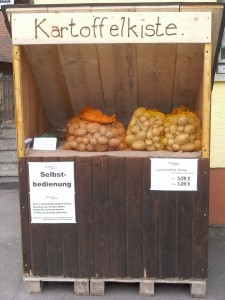
\includegraphics[width=0.3\textwidth,angle=0]{abb/Kartoffelkiste}
	\caption[Die Kartoffelkiste]{\glqq Kartoffelkiste\grqq{} \cite{Kartoffelkiste}}
	\label{fig:Kartoffelkiste}
\end{figure}


\begin{figure}[hh]
	\centering
	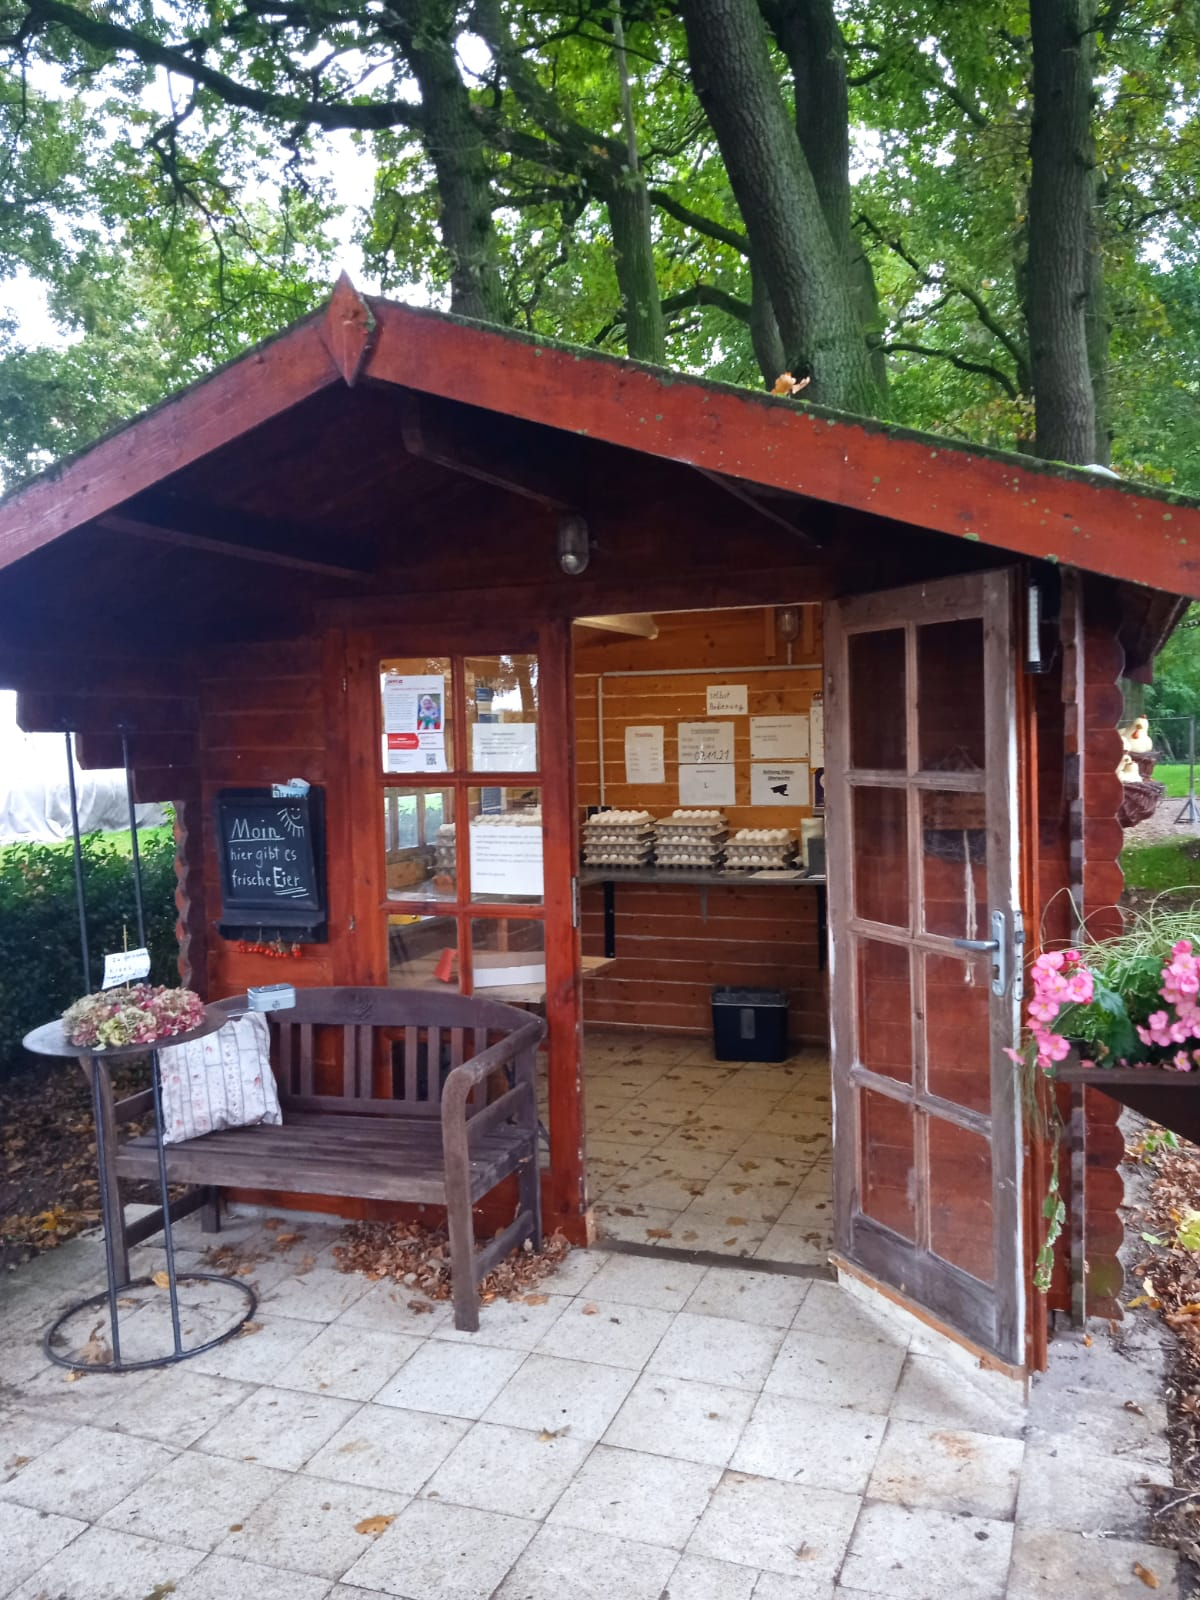
\includegraphics[width=0.3\textwidth,angle=0]{abb/Eierhaus}
	\caption[Eierhaus]{Eierhaus }
	\label{fig:Eierhaus}
\end{figure}


Der Begriff Selbstbedienung wird von \cite{Selbstbedienung} wie folgt definiert \glqq Verkaufsprinzip im Handel, bei dem der Kunde aus einem frei zugänglichen und griffbereit ausgestellten Warensortiment ohne Mitwirkung des Verkaufspersonals die von ihm gewählten Artikel zu den betrieblichen Inkassostellen transportiert.\grqq{} 
\\
\\
\\
Bei einem Kauf in einer Selbstbedienungshütte bezahlt der Kunde seine Ware 
selbstständig, ohne Verkaufspersonal und wirft das Geld in einen dafür vorgesehenen Behälter. Dieses kann zum Beispiel eine abschließbare Geldkassette mit Münzeinwurf sein.
\\
Der Stand bzw. der Ort, an dem die Waren angeboten werden, kann die unterschiedlichsten Bauweisen oder Formen aufweisen.

Auf dem Bild~\ref{fig:Kartoffelkiste} und dem Bild~\ref{fig:Eierhaus} sind zwei unterschiedliche Bauweisen zu sehen. Das Bild~\ref{fig:Kartoffelkiste} zeigt einen Straßenstand, auf dem zweiten Bild~\ref{fig:Eierhaus} ist eine Blockhütte zu sehen.


\subsection{Gesetzliche Grundlagen}\label{gesetzliche Grundlagen}

In diesem Kapitel werden einige gesetzliche Grundlagen vorgestellt. 
Es ist nicht möglich auf alle gesetzlichen Vorschriften einzugehen, da es zu viele unterschiedliche Reglungen gibt.
Außerdem werden die hier vorgestellten Vorschriften und Reglungen nicht im Detail erläutert. Für ausführlichere Informationen muss der Betreiber sich bei den zuständigen Stellen erkundigen. 
\\
\\
Als Erstes wird geklärt, was Direktvermarktung landwirtschaftlicher Erzeugnisse eigentlich bedeutet. \cite{gesetze1} schreibt \glqq Unter Direktvermarktung
versteht man die direkte Abgabe landwirtschaftlicher Produkte durch den Erzeuger auf dem Hof, auf dem Markt, an der Tür oder über eigene Hofläden an den Verbraucher.\grqq{} 
\\
\\
Werden nur \glqq selbsterzeugte unverarbeitete landwirtschaftliche Produkte, die als Urprodukte gelten vermarktet\grqq{}, ist dieses \glqq kein Gewerbe im Sinne der Gewerbeordnung\grqq{} erwähnt \cite{gesetze4}. Außerdem heißt es dort weiter \glqq werden (Ur-)Produkte für den Verkauf gereinigt, sortiert und hergerichtet (sogenannte erste Verarbeitungsstufe), so ist dies unschädlich.\grqq{}
\\
\\
\begin{table}[h]
	\centering
	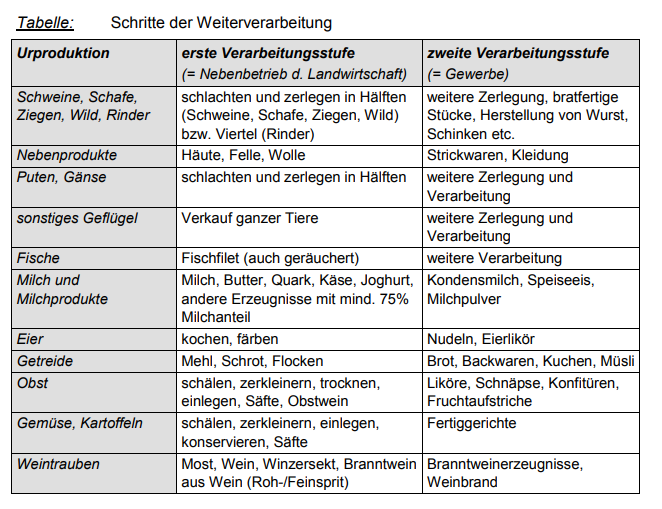
\includegraphics[width=0.8\textwidth,angle=0]{abb/urproduktion}
	\caption[Urproduktion, Schritte der Weiterverarbeitung]{Urproduktion, \glqq Schritte der Weiterverarbeitung\grqq{} \cite{gesetze2}}
	\label{tab:Urproduktion}
\end{table}


In der Tabelle~\ref{tab:Urproduktion} sind einige Urprodukte der ersten und zweiten Verarbeitungsstufe abgebildet. 
\\
Folgende Punkte führen zur Anzeigepflicht eines Gewerbes:\cite{gesetze2}


\begin{itemize}
	\item Der Verkauf von weiterverarbeiteten Produkten (zweite Verarbeitungsstufe) erzielt einen Umsatz von 10 Prozent des Gesamtumsatzes oder mehr des Betriebes.
	\item Verkauf von zugekaufter Ware, deren Umsatz 10 Prozent oder mehr des Betriebsumsatzes ausmachen.
	\item Verkauf und Urproduktion sind räumlich und personell getrennt. Ausgenommen hiervon ist ist der Marktstand.
\end{itemize}


Eine Vertrauenskasse wird laut \cite{gesetze5} wie folgt definiert \glqq Kasse, in die der Käufer selbständig den Kaufbetrag für die gekaufte Ware oder Leistung einzahlt, ohne dass in irgendeiner anderen Form der Verkäufer kassiert\grqq{}.
\\
\\
\cite{Bundesministerium} schreibt \glqq Als offene Ladenkasse gelten eine summarische, retrograde Ermittlung der Tageseinnahmen sowie manuelle Einzelaufzeichnungen ohne Einsatz technischer Hilfsmittel (BMF-Schreiben v. 19.6.2018).\grqq{} 
Der Begriff offene Ladenkasse bezieht sich nicht auf die Bauform der Kasse, sondern auf die Art, wie die Tageseinnahmen ermittelt werden.
\\ 
\\
Ein Landwirt, der direkt seine Produkte vermarktet, muss alle Einnahmen aufzeichnen. Diese müssen \glqq in einem Kassenbericht vollständig, richtig, zeitgerecht und geordnet aufgezeichnet werden\grqq{}, erwähnt \cite{gesetze7}. Dort heißt es weiter \glqq Laut Gesetz kommt bei Bargeldgeschäften der Grundsatz der Einzelauszeichnung zur Anwendung, [...] Da dieser Grundsatz in einem Hofladen [...] nicht praktikabel ist, gelten bestimmte Vereinfachungen.\grqq{} Diese Vereinfachungen besagen das es reicht, täglich die Summer der verkauften Waren und deren Einnahmen zu protokollieren.

\begin{table}[htb]
	\centering
	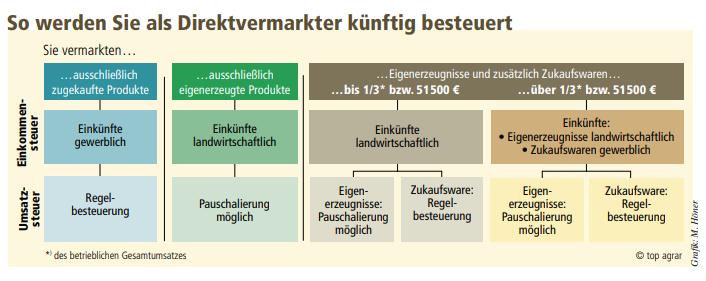
\includegraphics[width=1\textwidth,angle=0]{abb/versteuerung}
	\caption[Übersicht, Versteuerung Direktvermarkter]{Übersicht, Versteuerung Direktvermarkter \cite{gesetze3}}
	\label{fig:versteuerung}
\end{table}


In der Tabelle~\ref{fig:versteuerung} sind mögliche Versteuerungen zu sehen. Wichtig zu wissen, dies ist nur eine Übersicht, es kann möglicherweise sein, dass es im Steuerrecht abweichende Grenzen und Regeln gibt.
\\
\\
Nachfolgend werden ein paar weitere gesetzliche Reglungen aufgezählt, die eventuell beachtet werden müssen: Handwerksordnung, Gewerbeordnung, Steuerrecht, Baurecht, Lebensmittelhygienerecht, Qualitätskennzeichen, Verpackungsgesetz usw..


\subsection{Begriffsdefinitionen und Begriffserklärung}\label{begriffsdefinitionen}
Dieses Kapitel soll einen Überblick über verwendete Begriffsdefinitionen geben, zusätzlich werden einige Begriffe etwas genauer beschrieben.

\subsubsection{Client-Server-Architektur}\label{client-Server-Architektur}

Zunächst wird dargestellt, was ein Server ist, anschließend wird auf den Client eingegangen.
\\
\\
Laut \cite{clientServerModel} sind Server und Client keine reinen Hardwarekomponenten, sondern der Begriff \glqq Server und Client\grqq{} beschreibt Rollen.
\\
\\
\cite{clientServerModel} stellt fest das die Aufgabe eines Servers daraus besteht \glqq einen bestimmten Dienst lokal oder über das Netzwerk bereitzustellen.\grqq{}
Ein Server kann zum Beispiel Daten, Anwendungen, Dienste usw. bereitstellen. 
\\
\cite{win08}~[S.116] schreibt \glqq Eine Hardware- oder Softwarekomponente, der Dienste von einem Server in Anspruch nehmen kann (Client-Server-Prinzip) wird Client (Kunde) genannt.\grqq{} Dieses könnte zum Beispiel ein Computer sein, der die Dienste eines Servers in Anspruch nimmt. 
\\
Der Autor \cite{clientServerModel} erwähnt \glqq Das Client-Server-Modell ist ein Architekturkonzept zur Verteilung von Diensten und Aufgaben in einem Netzwerk. Dienste werden von Servern bereitgestellt und können von Clients genutzt werden.\grqq{}.

\begin{figure}[htb]
	\centering
	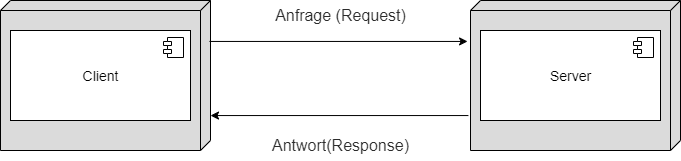
\includegraphics[width=1\textwidth,angle=0]{abb/Client-Server-Grundlagen}
	\caption[Vereinfachte Darstellung einer Kommunikation zwischen Client und Server]{Vereinfachte Darstellung einer Kommunikation \\ zwischen Client und Server}
	\label{fig:AB_Client-Server-Kommunikation_Grundlagen}
\end{figure}

Die Abbildung~\ref{fig:AB_Client-Server-Kommunikation_Grundlagen} stellt eine vereinfachte Darstellung einer Kommunikation zwischen Client und Server dar. Ein Client sendet eine Anfrage (Request) an einen Server, dieser verarbeitet die Anfrage und schickt eine Antwort (Response) zurück an den Client. Durchaus mehrere Clients können auf einen Server zugreifen. Außerdem kann sowohl der Client und der Server auf den selben Rechner ausgeführt werden.
\\
\cite{clientServerModel} schreibt, dass die Kommunikation und der Informationsaustausch über Protokolle geregelt wird. Bekannte und häufig verwendete Protokolle sind laut \cite{clientServerModel} das \glqq FTP (File Transfer Protokoll), HTTP (Hypertext Transfer Protocol) und das SNMP (Simple Network Management Protocol)\grqq{}.
\\
Ein Server baut nicht selbstständig eine Verbindung auf, sondern wartet auf eine Verbindungsanfrage.
\\
Ein typisches Beispiel einer Client-Server-Architektur ist ein Webbrowser, der auf einem Client läuft, dieser sendet eine Anfrage an einen Webserver und möchte eine bestimmte Internetseite aufrufen. Der Server prüft diese Anfrage und sendet die gewünschten Daten zurück.
\\
Einer der am häufigsten genutzten Webservern, ist der Apache HTTP Server\footnote{https://httpd.apache.org}. 

\subsubsection{REST-API}\label{RestAPI}

REST-API ist die Abkürzung von \glqq Representational State Transfer - Application Programming Interface \grqq{} beschreibt \cite{RESTAPI}.
Eine REST-API ist eine Programmierschnittstelle, mithilfe einer Schnittstelle ist es möglich, Daten und Informationen zwischen unterschiedlichen Systemen auszutauschen.
Der Autor \cite{RESTAPI2} erklärt \glqq Der als REST (oder auch ReST) bezeichnete Architekturansatz beschreibt, wie verteilte Systeme miteinander kommunizieren können.\grqq{}.
Gemäß \cite{RESTAPI} werden HTTP-Anfrage genutzt um auf Informationen zuzugreifen.
Die bekanntesten oft genutzte HTTP-Anfragen sind: \cite{RESTAPI2}

\begin{itemize}
	\itemsep0pt
	\item GET - Der Client fordert Daten vom Server an.
	\item POST - Der Server sendet die angeforderten Daten an den Client.
	\item PUT/PATCH - Der Server ändert vorhandene Daten.
	\item DELETE - Es sollen Daten vom Server gelöscht werden.
\end{itemize}

Schreibt das \cite{horn} alternativ auch das Nachrichtenprotokoll SOAP (Simple Object Access Protocol) verwendet werden kann.
\\
\\
\glqq Die Antworten werden oft im JSON-Format (JavaScript Object Notation) geliefert. Das Format ist sowohl für Menschen als auch Maschinen lesbar.\grqq{} berichtet \cite{RESTAPI3}.
\\
\lstset{language=java}
\begin{lstlisting}[frame=htrbl, caption={Beispiel für Daten im JSON Format}, label={lst:JSON}]
{
	"Benutzer": {
		"Name": [
		{
			"id": 1,
			"Vorname": "Christine",
			"Nachname": "Dall",
			"Administrator": true,
			"Adresse": null
		},
		{
			"id": 2,
			"Vorname": "Christin",
			"Nachname": "Ball",
			"Administrator": false,
			"Adresse": "Neuer Weg 6, 12345 Ort"
		},
		{
			"id": 3,
			"Vorname": "Christina",
			"Nachname": "Fall",
			"Administrator": false,
			"Adresse": null
		}
		]
	}
}
\end{lstlisting}

Im Listing~\ref{lst:JSON} zu sehen ist eine beispielhafte Datenstruktur. Dieses könnten zum Beispiel Daten, sein die der Client über eine Get-Anfrage erhält.
\\
\\
Außerdem wird vom Server auf jede Anfrage ein HTTP-Statuscode mitgesendet. Bekannte Statuscodes sind unter anderem: \cite{Statuscodes}
\begin{itemize}
	\itemsep0pt
	\item 200, OK
	\item 201, Erzeugt
	\item 400, Ungültige Anfrage
	\item 403, Verboten
	\item 404, Nicht gefunden
	\item 408, Anfrage-Zeitüberschreitung
	\item 409, Konflikt
	\item 500, Interner Server-Fehler
\end{itemize}

\subsubsection{Frameworks zur Realisierung einer Client-Server-Architektur}\label{frameworks zur Realisierung einer Client-Server-Architektur}

Ein Framework ist ein Programmiergerüst, dieses wird überwiegend in der objektorientierten Programmierung eingesetzt, dieses bildet den Rahmen und Anwendungsarchitektur einer Anwendung definiert \cite{Framework1}. Weiter heißt es dort \glqq Das Framework umfasst Bibliotheken, Komponenten und Laufzeitumgebungen und stellt die Designgrundstruktur für die Entwicklung zur Verfügung.\grqq{}.
\\
\\
Die Arbeit mit Frameworks bietet einige Vorteile. \cite{Framework2} erwähnt folgenden Vorteil, \glqq Wiederkehrende Aufgaben können schneller abgewickelt werden,\grqq{} bei der Verwendung von Frameworks spart sich der Programmierer Zeit und Aufwand.
\\
\\
Nachfolgend werden ein paar Frameworks und eine Bibliothek vorgestellt. 
\\
\\
\\
\\
\\
\\
Der Unterschied zwischen Bibliotheken und Frameworks ist \glqq Bei einer Bibliothek handelt es sich um eine Sammlung von Programmroutinen, die oft einen thematischen Zusammenhang aufweisen.\grqq{} schreibt \cite{AngularReactVergleich12}. Bibliotheken ergänzen Programmiersprachen um Funktionen. Ein Framework ist ein universelles Rahmenwerk und \glqq Um dieses rasch und übersichtlich einsetzen zu können, verwendet es nicht selten eine ergänzte oder variierte Syntax beziehungsweise eine eigene Programmiersprache und Struktur.\grqq{} wird noch ergänzend geschrieben von \cite{AngularReactVergleich12}. 
\\
\\
Vorgestellt werden Angular, React, Vue.js und Spring Boot. 
\\

\begin{longtable}{|l|l|l|}
	\hline
\rowcolor[gray]{0.6}	 & \multicolumn{2}{p{9.0cm}|}{ \textbf{Angular}} \\
\hline
	\hline
	Typ & \multicolumn{2}{l|}{Web-Framework } \\
	\hline
	Veröffentlichung & \multicolumn{2}{l|}{2016 entwickelt von Google Inc. \cite{AngularReactVergleich}} \\
	\hline
	Aktuelle Version & \multicolumn{2}{l|}{Angular 12.1.1 (Stand: 30.06.2021) } \\
	\hline
	Lizenz & \multicolumn{2}{l|}{MIT-Lizenz} \\
	\hline
	Betriebssystem & \multicolumn{2}{l|}{Plattformunabhängig} \\
	\hline
	Programmiersprache & \multicolumn{2}{l|}{TypeScript} \\
	\hline
	Webseiten die Angular nutzen & \multicolumn{2}{l|}{Youtube, PayPal} \\
	\hline
	\hline
	\multicolumn{3}{|p{14.0cm}|}{
	Bemerkung
	
Angular ist der Nachfolger von AngularJS und wurde komplett neu geschrieben. 

Der Autor \cite{AngularReactVergleich5} erwähnt das mit Angular komponentenbasiert entwickelt wird. 
		
	Eine Komponente besteht aus: \cite{AngularReactVergleich5}
	\begin{itemize}
		\itemsep0pt
		\item Template, enthält das HTML-Grundgerüst.
		\item Klasse, enthält die Logik die das Verhalten der Komponente steuert.
		\item Stylesheet, enthält das Layout.
	\end{itemize}
	} \\
	\hline
	\hline
	\multicolumn{3}{|p{12.0cm}|}{
		Vorteile
	
	\begin{itemize}
		\itemsep0pt
		\item Große Community \cite{AngularReactVergleich2}
		\item Große Typsicherheit, da TypeScript verwendet wird. \cite{AngularReactVergleich3}
		\item Erfordert keine zusätzlichen Bibliotheken \cite{AngularReactVergleich2}.
		\item \glqq Komponentenbasierte Architektur\grqq{} \cite{AngularReactVergleich5}
		\item Große Wiederverwendbarkeit der Komponenten \cite{AngularReactVergleich4}
		\item \glqq Zukunftssicher\grqq{} \cite{AngularReactVergleich5}
		\item Stabiles und verlässliches Framework \cite{AngularReactVergleich6}
		\item Hohe Performance. \cite{AngularReactVergleich5}
		\item Gut bei anspruchsvollen Backend-Anwendungen. \cite{AngularReactVergleich2}
		\item Verwendet HTML, CSS, Javascript, dieses ist vielen Entwicklern bereits bekannt. \cite{AngularReactVergleich3}
		\item Enthält viele Features (\glqq Dependency Injection, Templates, Routing, Ajax Requests\grqq{} \cite{AngularReactVergleich})
		\item Gute Dokumentation
	\end{itemize}} \\
	\hline
	\hline
	\multicolumn{3}{|p{12.0cm}|}{Nachteile
	
\begin{itemize}
	\itemsep0pt
	\item Hohe Einstiegshürde \cite{AngularReactVergleich2}
	\item Komplexes Framework \cite{AngularReactVergleich4}
	\item Abnehmender Community Support \cite{AngularReactVergleich4}
	\item Angular Versionen sind wenig kompatibel untereinander. \cite{AngularReactVergleich6}
	\item Geringere Flexibilität  \cite{AngularReactVergleich}
\end{itemize}} \\
	\hline
	\caption{Vorstellung des Frameworks Angular}
	\label{tab:dlsc}
\end{longtable}



\newpage


\begin{longtable}{|l|l|l|}
	\hline
	\rowcolor[gray]{0.6}	 & \multicolumn{2}{p{9.0cm}|}{ \textbf{React}} \\
	\hline
	Typ & \multicolumn{2}{l|}{JavaScript-Bibliothek} \\
	\hline
	Veröffentlichung & \multicolumn{2}{l|}{2013 entwickelt von Facebook Inc. \cite{AngularReactVergleich}} \\
	\hline
	Aktuelle Version & \multicolumn{2}{l|}{17.0.02 (Stand: 30.06.2021)  } \\
	\hline
	Lizenz & \multicolumn{2}{l|}{MIT-Lizenz} \\
	\hline
	Betriebssystem & \multicolumn{2}{l|}{Plattformunabhängig (Ab Version 3)} \\
	\hline
	Programmiersprache & \multicolumn{2}{l|}{JavaScript, ab Version 3 auch TypeScript } \\
	\hline
	Webseiten die React nutzen & \multicolumn{2}{l|}{Facebook, Instagram, Discord, Pinterest} \\
	\hline
	\hline
	\multicolumn{3}{|p{14.0cm}|}{
		Bemerkung
		
\cite{AngularReactVergleich} schreibt React besteht nur aus der 
View-Komponente. Diese Komponente beinhaltet \glqq den UI-Teil und die Logik der Applikation\grqq{}.
	
	} \\
	\hline
	\hline
	\multicolumn{3}{|p{12.0cm}|}{
		Vorteile
		
	\begin{itemize}
		\itemsep0pt
		\item Virtuelles DOM (Document Object Model), Veränderungen am eigentlich DOM werden dadurch klein gehalten. \cite{AngularReactVergleich3}
		\item Große Flexibilität \cite{AngularReactVergleich4}
		\item \glqq schlank, klein und elementar gehalten\grqq{} am Anfang sind nur Grundfunktionen verfügbar. \cite{AngularReactVergleich7}
		\item Beliebt, dadurch große Community vorhanden\cite{AngularReactVergleich4}
		\item Keine so hohe Einstiegshürde wie Angular. \cite{AngularReactVergleich3}
		\item Gute Unterstützung interaktiver Elemente. \cite{AngularReactVergleich2}
		\item Gute Dokumentation
		\item Es werden regelmäßig Updates veröffentlicht. 
	\end{itemize}} \\
	\hline
	\hline
	\multicolumn{3}{|p{12.0cm}|}{Nachteile
		
	\begin{itemize}
		\itemsep0pt
		\item Erfordert eventuell zusätzliche Bibliotheken. \cite{AngularReactVergleich}
		\item Wenig Futures, benötigte Packages müssen nachinstalliert werden. \cite{AngularReactVergleich}
		\item Template wird mit JSX geschrieben, Sprache muss eventuell gelernt werden. \cite{AngularReactVergleich7}
		\item Der Einsatz lohnt sich nur für Seiten die viele Interaktive Elemente enthalten. \cite{AngularReactVergleich3}
	\end{itemize}} \\
	\hline
		\caption{Vorstellung der Bibliothek React}
	\label{tab:react}
\end{longtable}





\begin{longtable}{|l|l|l|}
	\hline
	\rowcolor[gray]{0.6}	 & \multicolumn{2}{p{9.0cm}|}{ \textbf{Vue.js}} \\
	\hline
	Typ & \multicolumn{2}{l|}{Web-Framework} \\
	\hline
	Veröffentlichung & \multicolumn{2}{l|}{2014 entwickelt Evan You \cite{AngularReactVergleich}} \\
	\hline
	Aktuelle Version & \multicolumn{2}{l|}{17.0.02 (Stand: 30.06.2021)  } \\
	\hline
	Lizenz & \multicolumn{2}{l|}{MIT-Lizenz} \\
	\hline
	Betriebssystem & \multicolumn{2}{l|}{Plattformunabhängig (Ab Version 3)} \\
	\hline
	Programmiersprache & \multicolumn{2}{l|}{JavaScript, ab Version 3 auch TypeScript } \\
	\hline
	Webseiten die Vue.js nutzen & \multicolumn{2}{l|}{Gitlab, Nintendo, Shopware} \\
	\hline
	\hline
	\multicolumn{3}{|p{14.0cm}|}{
Bemerkung
		
Bei Vue.js\glqq handelt es sich hier um eine monolithische Lösung, die dem Entwickler alle nötigen Tools für eine umfassende Applikation anbietet.\grqq{} \cite{AngularReactVergleich7}
	} \\
	\hline
	\hline
	\multicolumn{3}{|p{12.0cm}|}{
		Vorteile
		
	\begin{itemize}
		\itemsep0pt
		\item Leichter Einsieg \cite{AngularReactVergleich8}
		\item Modularer Aufbau  \cite{AngularReactVergleich9}
		\item Schlanker Aufbau, unterschiedliche Module können hinzugefügt werden.\cite{AngularReactVergleich10} 
		\item \glqq 50 \% weniger Renderzeit: im Vergleich zu anderen Frameworks.\grqq{}\cite{AngularReactVergleich11}
		\item Virtuelles DOM (Document Object Model), Veränderungen am eigentlich DOM werden dadurch klein gehalten. \cite{AngularReactVergleich9}
		\item Ist nur 10 kB groß.(Version 3) \cite{AngularReactVergleich11}
	\end{itemize}} \\
	\hline
	\hline
	\multicolumn{3}{|p{12.0cm}|}{Nachteile
		
	\begin{itemize}
		\itemsep0pt
		\item Kleine Community \cite{AngularReactVergleich4}
		\item Kleines Entwicklerteam \cite{AngularReactVergleich9}
		\item Wenig Erweiterungen. \cite{AngularReactVergleich12}
	\end{itemize}} \\
	\hline
		\caption{Vorstellung des Frameworks Vue.js}
	\label{tab:vue}
\end{longtable}


\newpage

\begin{longtable}{|l|l|l|}
	\hline
	\rowcolor[gray]{0.6} & \multicolumn{2}{p{9.0cm}|}{ \textbf{Spring Boot}} \\
	\hline
	Typ & \multicolumn{2}{l|}{Application Framework} \\
	\hline
	Veröffentlichung & \multicolumn{2}{l|}{2002 entwickelt von Rod Johnson, ab September 2009 VMware} \\
	\hline
	Aktuelle Version & \multicolumn{2}{l|}{ 5.3.8 (Stand: 30.06.2021)  } \\
	\hline
	Lizenz & \multicolumn{2}{l|}{Apache-Lizenz} \\
	\hline
	Programmiersprache & \multicolumn{2}{l|}{Java, Kotlin, Groovy } \\
	\hline
	\multicolumn{3}{|p{14.0cm}|}{
		Bemerkung
				
\cite{Spring2} definiert \glqq Das Spring Framework ist ein schlankes Open-Source-Framework für Java. Mittels Dependency Injection und aspektorientierter Programmierung soll es einen insgesamt leichteren und besser wartbaren Programmcode ermöglicht.\grqq{}
	} \\
	\hline
	\hline
	\multicolumn{3}{|p{12.0cm}|}{
		Vorteile
		
		\begin{itemize}
		\itemsep0pt
		\item MVC-Architektur
		\item Dependency Injection
		\item Aspektorientierte Programmierung 
		\item Flexible Modulsammlung 
		\item Große Community
		\item Ausführliche Dokumentation
		\item Flache Lernkurve \cite{Spring3}
		\item Unterstützt viele Datenbanken  \cite{Spring3}
	\end{itemize}} \\
	\hline
	\hline
	\multicolumn{3}{|p{12.0cm}|}{Nachteile
		
	\begin{itemize}
		\itemsep0pt
		\item Höhere Code-Ausführungszeit
		\item Erfordert Einarbeitungszeit
	\end{itemize}} \\
	\hline
		\caption{Vorstellung des Frameworks Spring Boot}
	\label{tab:spring}
\end{longtable}

\subsection{SQL-Datenbank}\label{sQL-Datenbank}
Datenbanken werden in fast jeder größeren Softwareanwendung in der IT verwendet. 
In einer Datenbank werden Daten bereitgestellt und gespeichert, die für den Betrieb der Software nötig sind.
Das können zum Beispiel folgende Daten sein: Benutzername, Passwort, Artikelinformationen usw..
\\
\\
\\
Gemäß \cite{win08} ~[S.55] ist eine Datenbank, eine strukturierte, dauerhaft elektronisch gespeicherte Sammlung von Datenmengen. Eine Datenbank kann mithilfe eines Datenbankmanagementsystems (DBMS) verwaltet werden. Bekannte DBMS sind unter anderem MySQL\footnote{https://www.mysql.com/de/} und Oracle\footnote{https://www.oracle.com/database/}. 
\\
\\
In der Praxis werden unterschiedliche Datenbankmodell verwendet, eines der am häufigsten genutzten Systeme ist das relationale Datenbankmodell. 
\cite{t3rationaleDatenbank} schreibt, dass eine relationale Datenbank aus unterschiedlich vielen Tabellen bestehen kann. Es werden logisch zusammenhängende Daten miteinander verknüpft (in Relation gesetzt). \cite{oracleDB} beschreibt eine relationale Datenbank als \glqq ein Typ von Datenbanken, der die Speicherung und den Zugriff auf miteinander verbundener Datenpunkte ermöglicht.\grqq{}.
\\
\\
Mithilfe einer Datenbanksprache lassen sich unter anderem Daten einfügen, löschen oder verändern. Diese Datenbankoperationen sind auch unter dem Begriff CRUD bekannt. \cite{db2222} erklärt das die Abkürzung sich aus den Begriffen Create, Read, Update, Delete zusammensetzt.
\\
\\
In dieser Praxisarbeit wird SQL verwendet, die Abkürzung steht für Structured Query Language. Gemäß \cite{datenbankenVerstehen} ist SQL \glqq eine Datenbanksprache zur Erstellung von Datenbankstrukturen in relationalen Datenbanken sowie zum Bearbeiten und Abfragen der darauf basierenden Datenbeständen.\grqq{}.
\\
\cite{Lub17} erwähnt das SQL keine vollwertige Programmiersprache ist, das heißt hiermit können keine kompletten Anwendungen erstellt werden, aber SQL lässt sich gut mit Programmiersprachen kombinieren. \cite{bitfarm} schreibt das SQL, durch die weite Verbreitung zum Standard in Deutschland geworden ist.
\\
\\
Laut \cite{Lub17} lassen sich die SQL-Befehle in drei unterschiedliche Kategorien aufteilen.
Die drei Kategorien sind, DML-Befehle (Data Manipulation Language Befehle), DDL-Befehle (Data Definition Language Befehle) und DCL-Befehle (Data Control Language Befehle).
\\
DML-Befehle werden zum Bearbeiten, Löschen und Einfügen verwendet. Bekannte und oft verwendete Befehle werden in der Tabelle~\ref{tab:dml} dargestellt.
\\
DDL-Befehle sind dazu geeignet, die Struktur der Datenbank zu steuern.
Bekannte DDL-Befehle sind in der Tabelle~\ref{tab:ddl} abgebildet.
\\
Außerdem gibt es noch die DLC-Befehle, diese Befehle helfen bei der Rechteverwaltung. Beispiele hierfür sind in der Tabelle~\ref{tab:dlc} zusehen. 
\\
\\
\\
In den nachfolgenden Tabellen werden einige Beispielbefehle, entnommen aus \cite{w3SQL}, aufgezeigt.
\\
\\
\begin{table}[h]
	\begin{tabular}{|p{7cm}|p{7cm}|}
		\hline
		\textbf{Befehl} & \textbf{Beschreibung} \\
		\hline
		SELECT * FROM Tabellenname & Mit diesem Befehl werden Daten aus Tabellen ausgelesen. \\
		\hline
		INSERT INTO Tabellenname (Spaltenname1, Spaltenname2, ... ) VALUES (Wert1, Wert 2, ...)	 & Dieser Befehl fügt Daten in die Tabelle ein. \\
		\hline
		DELETE FROM Tabellenname WHERE Bedienung & Mithilfe dieses Befehls werden Daten aus der Tabelle gelöscht. \\
		\hline
		UPDATE Tabellenname SET (Spalte1 = Wert1, Spalte2 = Wert2, ...) WHERE Bedienung  & Dieser Befehl sorgt dafür, dass Daten in der Tabelle aktualisiert werden. \\
		\hline
	\end{tabular}
	\caption{DML-Befehle}
	\label{tab:dml}
\end{table}
\\  

\begin{table}[h]
	\begin{tabular}{|p{7cm}|p{7cm}|}
		\hline
		\textbf{Befehl} & \textbf{Beschreibung} \\
		\hline
		CREATE DATABASE Datenbankname & Mithilfe dieses Befehls wird eine neue Datenbank erstellt. \\
		\hline
		CREATE TABLE Tabellenname (Spaltenname1 Datentyp1, Spaltenname2 Datentyp2, ...) & Dieser Befehl sorgt dafür, dass eine neue Tabelle angelegt wird.\\
		\hline
		DROP TABLE Tabellenname & Soll eine Tabelle gelöscht werden, kann dieser Befehl genutzt werden.\\
		\hline
		ALTER TABLE Tabellename ADD Spaltenname Datentyp & Es wird eine neue Spalte in der Tabelle eingefügt, sobald dieser Befehl genutzt wird. \\
		\hline
	\end{tabular}
	\caption{DDL-Befehle}
	\label{tab:ddl}
\end{table}


\begin{table}[h]
	\begin{tabular}{|p{7cm}|p{7cm}|}
		\hline
		\textbf{Befehl} & \textbf{Beschreibung} \\
		\hline
		GRANT Privileg  ON Datenbankname TO \{Benutzername |PUBLIC |Rollenname\}[WITH GRANT OPTION] & Die Zuggriffrechte werden mithilfe dieses Befehls gewährt. \\
		\hline
		REVOKE Privileg ON Datenbankname FROM \{Benutzername |PUBLIC |Rollenname\} &  Dieser Befehl entzieht dem Benutzer Zugriffsrechte.\\
		\hline
	\end{tabular}
	\caption{DLC-Befehle}
	\label{tab:dlc}
\end{table}

\newpage

\section{Anforderungsanalyse}\label{anforderungsanalyse}

In diesem Kapitel wird eine Anforderungsanalyse durchgeführt, Ziel ist es, die Anforderungen für die zu erstellte Anwendung zu ermitteln. 
Zunächst muss allerdings eine kleine Problemanalyse durchgeführt werden. Diese Analyse dient dazu, das Problem näher zu erläutern.
\\
\\
Unterschieden wird zwischen zwei Anforderungsarten.\cite{FunktionaleAnforderungen}.

\begin{itemize}
	\itemsep0pt
	\item Mithilfe funktionaler Anforderungen wird festgelegt was das System tun soll. 
	\item Nichtfunktionale Anforderungen legen fest, wie das System etwas tun soll. 
\end{itemize}

\subsection{Problemanalyse}\label{problem}
Zuerst wird erläutert, welches Problem die Anwendung lösen soll.
\\
Es muss jeden Tag, an dem Ware verkauft wird, eine Abrechnung erstellt werden. Diese Anwendung soll dabei helfen, diesen Vorgang zu vereinfachen. Genauer gesagt soll die Anwendung helfen, einen Überblick über die verkaufte Ware zu erhalten. Diese soll an einem Fallbeispiel verdeutlicht werden.
\\
\\
In einer Hütte werden unter anderem Eier verkauft. Am Tagesbeginn befinden sich bereits 254 Eier in der Hütte. Im Laufe des Tages werden insgesamt 480 Eier in die Hütte gebracht. Die Eier werden von unterschiedlichen Personen in unterschiedlicher Anzahl in die Hütte gestellt. Jeder dieser Personen muss immer irgendwo die genaue Stückzahl festhalten. Am Ende des Tages wird eine Abrechnung erstellt. Dazu werden die in der Hütte vorhanden Eier gezählt, dieses sind 142 Stück, anschließend wird folgende Rechnung aufgestellt.
\\
\\
Anzahl der vorhandenen Eier vom Vortag + Summe der Eier aus Zugängen - Anzahl der aktuell gezählten und noch in der Hütte vorhanden Eier = Summe der theoretisch verkauften Eier. 
\\
\\
254 Eier + 480 Eier - 142 Eier = 592 verkaufte Eier
\\
\\
Hierbei sind Diebstähle usw. nicht berücksichtigt. Anschließend wird das Geld in der Kasse gezählt und mit der Summe verglichen, die es theoretisch sein sollte.  
\\
\\
Aufwendiger wird dieser Vorgang, sobald mehr als eine Warensorte angeboten wird. Einige Erzeuger betreiben auch mehrere Selbstbedienungsstände, für jeden davon muss eine separate Abrechnung erstellt werden. 

\subsection{Funktionale Anforderungen}\label{funktionale_Anforderungen}

Aus der Problemstellung lassen sich folgende funktionale Anforderungen ableiten.
\\
\\
Funktion: \textbf{Benutzer und Selbstbedienungsstand neu anlegen}\\
Beschreibung: Es wird ein neuer Benutzer angelegt. Der Benutzer erhält Adminrechte. Es wird überprüft, ob der Benutzername vergeben ist, ebenso ob das Passwort den Anforderungen entspricht. Außerdem wird überprüft, ob der Name des Selbstbedienungsstandes bereits genutzt wird.


\noindent\rule{\textwidth}{1pt}


Funktion: \textbf{Benutzername oder Passwort ändern}\\
Beschreibung: Der Benutzername bzw. das Passwort des Benutzers wird geändert. Es wird überprüft, ob der Benutzername bereits vergeben ist bzw. ob das Passwort den Anforderungen entspricht.


\noindent\rule{\textwidth}{1pt}

Funktion: \textbf{Benutzer löschen}\\
Beschreibung: Der Benutzer wird gelöscht.

\noindent\rule{\textwidth}{1pt}

Funktion: \textbf{Mehrbenutzer}\\
Beschreibung: Einem Selbstbedienungsstand können mehrere Benutzer zugeordnet werden. 


\noindent\rule{\textwidth}{1pt}

Funktion: \textbf{Selbstbedienungsstand anlegen}\\
Beschreibung: Es wird ein neuer Selbstbedienungsstand angelegt. Zuvor wird überprüft, ob bereits ein Selbstbedienungsstand mit gleichen Namen existiert.


\noindent\rule{\textwidth}{1pt}

Funktion: \textbf{Selbstbedienungsstand, Name ändern}\\
Beschreibung: Der Name des Selbstbedienungsstands wird geändert. Nur der Admin des Selbstbedienungsstandes kann diesen ändern. Es wird überprüft, ob bereits ein Selbstbedienungsstand mit diesem Namen erstellt worden ist.


\noindent\rule{\textwidth}{1pt}


Funktion: \textbf{Selbstbedienungsstand löschen}\\
Beschreibung: Der Selbstbedienungsstand wird gelöscht. Nur der Admin des Selbstbedienungsstandes kann diesen löschen.


\noindent\rule{\textwidth}{1pt}

Funktion: \textbf{Selbstbedienungsstand, Benutzer hinzufügen}\\
Beschreibung: Der Admin fügt weitere Benutzer hinzu, diese Nutzer gehören dann ebenfalls zu dem Selbstbedienungsstand. 

\noindent\rule{\textwidth}{1pt}
\\
\\
Funktion: \textbf{Selbstbedienungsstand, neuen Benutzer erstellen}\\
Beschreibung: Der Admin legt einen weiteren Benutzer an, diese Nutzer gehören dann ebenfalls zu dem Selbstbedienungsstand. 


\noindent\rule{\textwidth}{1pt}

Funktion: \textbf{Ware anlegen}\\
Beschreibung: Der Admin kann neue Ware anlegen. Folgende Wareninformationen sollen hinterlegt sein: Warenname, Einheit, Preis, Bemerkung, aktuell im Verkauf. 
Sobald eine neue Ware angelegt wird, erhält diese automatisch den Status im Verkauf.


\noindent\rule{\textwidth}{1pt}

Funktion: \textbf{Ware löschen}\\
Beschreibung: Der Admin kann eine Ware löschen. 


\noindent\rule{\textwidth}{1pt}

Funktion: \textbf{Warendaten ändern}\\
Beschreibung: Ein Administrator kann die Warendaten einer Ware ändern.

\noindent\rule{\textwidth}{1pt}


Funktion: \textbf{Warenbewegung eingeben}\\
Beschreibung: Ein Anwender kann für jede Ware den Wareneingang oder Warenabgang festhalten, und dieser wird gespeichert.

\noindent\rule{\textwidth}{1pt}


Funktion: \textbf{Tagesabschluss erstellen}\\
Beschreibung: Es wird eine Tagesabrechnung erstellt. Aus dieser geht hervor, wie viele Waren verkauft worden sind und wie hoch die Einnahmen sind. Dabei werden Diebstahl usw. nicht berücksichtigt.



\subsection{Nichtfunktionale Anforderungen}\label{nichtfunktionale_Anforderungen}

Nachfolgend werden Nichtfunktionale Anforderungen vorgestellt. 
\\
\begin{itemize}
		\itemsep0pt
	\item Technische Anforderungen
		\begin{itemize}
		\item Das System sollte erweiterbar sein (App, Desktop-Anwendung).
		\item Es sollte nach Möglichkeit auf jeder Plattform lauffähig sein.
		\item Die Anwendung soll Standortunabhängig sein.
		\item Die Anwendung sollte von möglichst vielen unterschiedlichen Geräten (z.B. Smartphone, Destop-Pc usw.) bedienbar sein. (Responsive-Webdesign)
		\item Tagesabschluss als PDF-Dokument.
		\end{itemize}
	\item Sicherheit\textit{}
		\begin{itemize}
		\item Es soll JSON Web Token genutzt werden.
		\item Passwort soll verschlüsselt in der Datenbank gespeichert werden.
		\end{itemize}
	\item Ergonomische Anforderungen
	\begin{itemize}
		\item Leichte Bedienbarkeit.
		\item Übersichtliches Design.
		\item Deutsche Textausgabe.
	\end{itemize}
\end{itemize}


\subsection{Zusammenfassung der Anforderungen}\label{zusa}
In diesem Kapitel sind nachfolgend alle Anforderungen nochmals kurz aufgezählt.
\\

\begin{table}[htbp]
	\centering
\begin{tabular}{|c|c|}
		\hline
	Nr. & Anforderung \\
	\hline
	1 & Benutzer und Selbstbedienungsstand neu anlegen \\
	\hline
	2 & Benutzername oder Passwort ändern \\
	\hline
	3 & Benutzer löschen \\
	\hline
	4 & Mehrbenutzer \\
\hline	
	5 & Selbstbedienungsstand anlegen \\
	\hline
	6 & Selbstbedienungsstand, Name ändern \\
	\hline
	7 & Selbstbedienungsstand löschen \\
	\hline
	8 & Selbstbedienungsstand, Benutzer hinzufügen \\
	\hline
	9 & Selbstbedienungsstand, neuen Benutzer erstellen \\
	\hline
	10 & Ware anlegen \\
	\hline
	11 &  Ware löschen\\
	\hline
	12 &  Warendaten ändern\\
	\hline
	13 & Warenbewegung eingeben \\
	\hline
	14 & Tagesabschluss erstellen \\
	\hline
	15 & JSON Web Token  \\
	\hline
	16 &  Verschlüsseltes Passwort in Datenbank speichern\\
	\hline
	17 & Erweiterbares System \\
	\hline
	18 &  Plattformunabhängig\\
	\hline
	19 &  Standortunabhängig\\
	\hline
	20 & Responsive-Webdesign \\
	\hline
	21 &  Tagesabschluss als PDF-Dokument\\
	\hline
	22 & Leichte Bedienbarkeit \\
	\hline
	23 &  Übersichtliches Design\\
	\hline
	24 &  Deutsche Textausgabe\\
	\hline
\end{tabular}
	\caption{Zusammenfassung der Anforderungen}
\label{tab:zu}
\end{table}

\newpage

\section{Konzeption}\label{konzeption}

In diesem Kapitel werden einige Konzeptionsentwürfe dargestellt und erläutert. 
Zuerst wird der allgemeine Architekturentwurf präsentiert. Im Anschluss folgen die Entwürfe für Server, Datenbank, Client und Schnittstellen.

\subsection{Allgemeiner Architekturentwurf}\label{allgemeiner_Architekturentwurf}

In diesem Unterkapitel wird der allgemeine Architekturentwurf erläutert.
\\
\\
Für das Projekt wird eine Client-Server-Architektur gewählt, da aus der Anforderungsanalyse hervorgeht, dass die Anwendung auf möglichst vielen Geräten standortunabhängig lauffähig sein soll. Außerdem soll in Zukunft die Möglichkeit bestehen, dass eine App eingebunden werden kann.
\\
\\

\begin{figure}[htb]
	\centering
	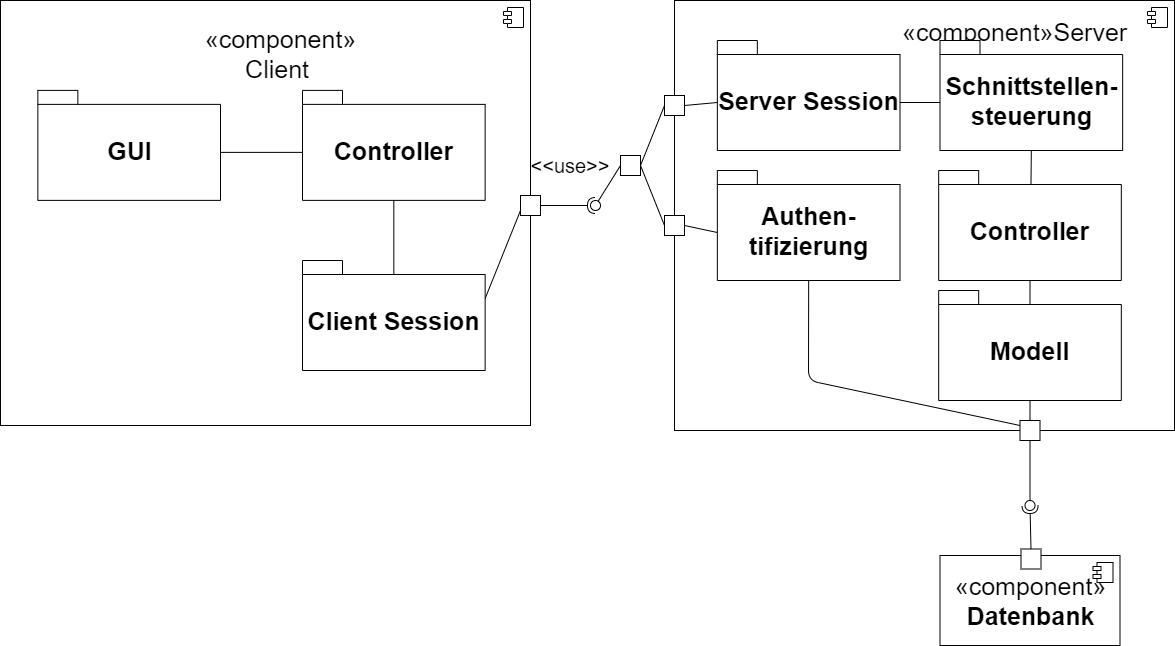
\includegraphics[width=1\textwidth,angle=0]{abb/Komponentendiagramm}
	\caption[Komponentendiagramm]{Komponentendiagramm}
	\label{fig:Komponentendiagramm}
\end{figure}

Die Abbildung~\ref{fig:Komponentendiagramm} zeigt ein Komponentendiagramm, mit folgenden drei Komponenten Client, Server und Datenbank. 
Die Darstellung ist eine vereinfachte Abbildung, diese dient dazu einen ersten Überblick über das zu entwerfende System zu erhalten. 
\\
\\
Der Client enthält drei Pakete GUI, Controller und Client Session. 
\\
GUI (Graphical User Interface) beinhaltet die Grafische Benutzeroberfläche.
\\
Sobald ein Benutzer eine Eingabe tätigt, wird diese an den Controller gesendet. Der Controller ist dafür zuständig, die Eingaben zu prüfen, weiterzuleiten, zu ändern usw.. Sollte der Controller Daten vom Server benötigen, wird eine Session (Verbindung) zum Server aufgebaut, dafür ist das Paket Client Session zuständig.
\\
\\
Der Server beinhaltet fünf Pakete Server Session, Authentifizierung, Schnittstellensteuerung, Controller und Modell. 
\\
Sollte der Benutzer bislang noch kein Account angelegt haben oder die Zugriffsberechtigung (Token) ist abgelaufen, muss eine neue Authentifizierung durchgeführt werden. Hierfür ist das Paket Authentifizierung zuständig.
\\
Ansonsten wird mithilfe einer Server Session eine Verbindung aufgebaut. 
 \\
Das Paket Schnittstellensteuerung verwaltet eingehende Anfragen und leitet diese an den Controller weiter. Das Paket Controller steuert die eingehenden Anfragen. Sobald Anfragen Daten ändern, löschen, hinzufügen oder abfragen, sendet der Controller diese an das Paket Modell. Die Pakete Authentifizierung und Modell können eine Verbindung zur Datenbank aufbauen.

\subsection{Entwurf der Datenbank}\label{entwurf_der_Datenbank}

In diesem Kapitel werden die einzelnen Entwurfsschritte, die zum Erstellen der Datenbank notwendig sind, erläutert. 
Wie bereits in Kapitel~\ref{sQL-Datenbank} erwähnt, wird eine rationale Datenbank umgesetzt.

\subsubsection{Normalisierung der Datenbank}\label{normalisierung}

Es liegt nach der Anforderungsanalyse folgende Ausgangssituation vor. Nachfolgende Daten sollen unter anderem gespeichert werden:
Benutzername, Passwort, Benutzerrolle, Selbstbedienungsstandname, Datum, Warenname, Preis(€), Wareneingang, gezählte Waren, verkaufte Waren, Einnahmen(€).
\\
\\
Aus diesen Daten wird ein Entity-Relationship-Modell (ER-Modell) erstellt, dieses beinhaltet Entitäten, Attribute, Beziehungen, Primärschlüsseln, zusammengesetzte Primärschlüssel und Fremdschlüssel.
Aus dem ER-Modell werden im Anschluss Tabellen erstellt.
\\
Eine Entität (Rechteck) beschreibt ein Objekt, daraus wird später der Tabellenname. Die Attribute (Ellipsen) werden in Tabellenspalten überführt.
\\
Ein Primärschlüssel (unterstreichendes Attribut) dient dazu, die einzelnen Datensätze auch Tupel genannt eindeutig zu identifizieren.
Bei einem zusammengesetzten Primärschlüssel werden zwei oder mehr Attribute zur eindeutigen Erkennung eines Tupels verwendet.
Der Fremdschlüssel verweist auf ein anderes Attribute, dieses muss ein Primärschlüssel sein. Dadurch können Tabellen miteinander in Beziehung (Raute) gebracht werden.

\begin{figure}[htb]
	\centering
	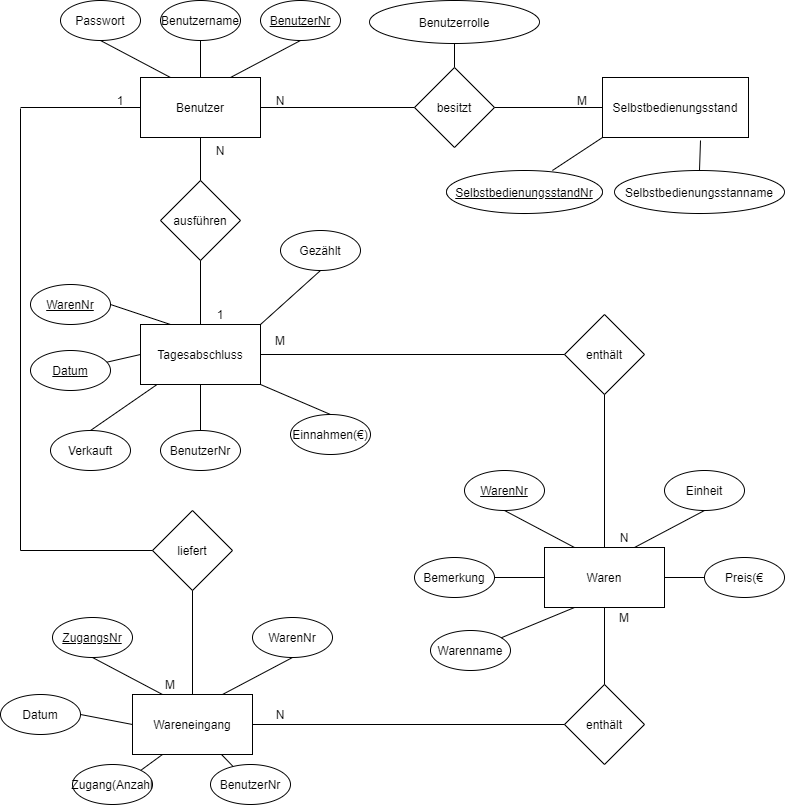
\includegraphics[width=1\textwidth,angle=0]{abb/ER-Modell}
	\caption[ER-Modell]{ER-Modell}
	\label{fig:ER Modell}
\end{figure}


In der Abbildung~\ref{fig:ER Modell} ist das erstellte ER-Modell abgebildet. Daraus werden die Tabellen abgeleitet. 

\cite{DBREdun} empfiehlt es, eine Datenbank so zu gestalten das \glqq Redundanzen, Inkonsistenzen und Anomalien\grqq{} vermieden werden. 
Dieses soll mithilfe der Normalformen umgesetzt werden.
Es existieren bis zu fünf Normalformen, in der Praxis werden oftmals nur die ersten drei Normalformen gebildet, erwähnt \cite{DB2}.
Es sollen nachfolgend drei aufeinander aufbauende Normalisierungschritte durchgeführt werden.

\cite{relaDatenbank} zufolge sollten die folgenden Datenbankanforderungen eingehalten werden:

\begin{itemize}
	\itemsep0pt
	\item Eindeutige Struktur, jeder Datensatz muss eindeutig zu identifizieren sein.
	\item Redundanzfrei, nach Möglichkeit sollten keine Daten mehrfach vorhanden sein.
	\item Keine Inkonsistenzen, keine Widersprüchlichkeit zwischen den Daten.
\end{itemize} 


Die Voraussetzung für die erste Normalform ist, dass alle Tabellenspalten gleichartige Werte enthalten und alle Daten atomar sind.
Das heißt, eine Tabellenspalte darf keine unterschiedlichen Typen enthalten, z.B. Betrag in Euro und Betrag in Cent. 
Außerdem müssen die Daten atomar sein, es ist nicht erlaubt mehrere Werte in einem Feld zu haben z.B. Straße, Postleitzahl, Ort.
\\
\\
Der Autor \cite{DB2} schreibt, sobald eine Tabelle in der ersten Normalform und jedes Nichtschlüsselattribut vom Primärschlüssel funktional abhängig ist, befindet sich die Tabelle in der zweiten Normalform. Dieses trifft bereits zu, z. B. der Benutzername ist abhängig von der BenutzerNr..
\\
\\
Bei der Erstellung der Tabellen wird darauf geachtet das diese direkt in der 2. Normalform vorliegen. 

\begin{table}[H]
	\centering
	\begin{tabular}{|c|c|c|}
		\hline
		\underline{BenutzerNr} & Benutzername & Passwort \\
		\hline
		1 & Christine &  12345\\
		\hline
		2 & ADE &  asdfg\\
		\hline
		3 & Hugo &  yxcvb\\
		\hline
	\end{tabular}
	\caption{Die Tabelle Benutzerdaten in der 2. Normalform.}
	\label{tab: Benutzerdaten 2.NF}
\end{table}

\begin{table}[H]
	\centering
	\begin{tabular}{|c|c|}
		\hline
		\underline{SelbstbedienungsstandNr} & Selbstbedienungsstandname \\
		\hline
		1 & Eierhütte \\
		\hline
		2 & Kartoffelhaus \\
		\hline
		3 & Stand1 \\
		\hline
	\end{tabular}
	\caption{Die Tabelle Selbstbedienungsstand in der 2. Normalform.}
	\label{tab: Selbstbedienung 2.NF}
\end{table}

\begin{table}[H]
	\centering
	\begin{tabular}{|c|c|c|}
		\hline
		\underline{SelbstbedienungsstandNr} & \underline{BenutzerNr} & Benutzerrolle \\
		\hline
		1 & 1 &  Admin\\
		\hline
		2 & 1 &  User\\
		\hline
		3 & 2 &  Admin\\
		\hline
		3 & 3 &  Admin\\
		\hline
	\end{tabular}
	\caption{Die Tabelle Selbstbedienungsstand-Nutzer in der 2. Normalform.}
	\label{tab: Selbstbedienung-Nutzer 2.NF}
\end{table}

Die Tabellen ~\ref{tab: Benutzerdaten 2.NF}, ~\ref{tab: Selbstbedienung 2.NF} und ~\ref{tab: Selbstbedienung-Nutzer 2.NF} beinhalten die Benutzerdaten und Selbstbedienungsstanddaten. Es wird davon ausgegangen das ein Selbstbedienungsstand mehrere Benutzer haben kann, gleichzeitig kann ein Nutzer mehrere Selbstbedienungsstände betreiben, dieses wird mithilfe der Tabelle~\ref{tab: Selbstbedienung-Nutzer 2.NF} umgesetzt.

\begin{table}[H]
	\centering
	\begin{tabular}{|c|c|c|c|c|}
		\hline
		\underline{WarenNr} & Warenname & Einheit & Preis(€)& Bemerkung \\
		\hline
		1 & Ei & Stück &  0,20 & \\
		\hline
		2 & Kartoffeln & KG & 5 & Sorte Annabelle \\
		\hline
	\end{tabular}
	\caption{Die Tabelle Waren in der 2. Normalform.}
	\label{tab: Waren 2.NF}
\end{table}


\begin{table}[H]
	\centering
	\begin{tabular}{|c|c|c|c|c|}
		\hline
		\underline{WareneingangsNr} & Datum & Wareneingang(Anzahl) & WarenNr & BenutzerNr \\
		\hline
		1 & 25.07.2021 & +100 & 2 & 1 \\
		\hline
		2 & 25.07.2021  & +80 & 1 & 1 \\
		\hline
		3 & 26.07.2021  & +60 & 2 & 1 \\
		\hline
		4 & 26.07.2021  &+5 & 2 &  2\\
		\hline
	\end{tabular}
	\caption{Die Tabelle Wareneingang in der 2. Normalform.}
	\label{tab: Wareneingang 2.NF}
\end{table}


\begin{table}[H]
	\centering
	\begin{tabular}{|c|c|c|c|c|c|}
		\hline
		\underline{Datum} & \underline{WarenNr} & BenutzerNr & Gezählt & Verkauft & Einnahmen(€) \\
		\hline
		25.07.2021 & 1 & 1 & 231 & 251 & 50,20 \\
		\hline
		26.07.2021 & 1 & 1 & 52 & 239 & 47,80 \\
		\hline
		26.07.2021 & 2 & 1 & 3 & 2 & 10 \\
		\hline
	\end{tabular}
	\caption{Die Tabelle Tagesabschluss in der 2. Normalform.}
	\label{tab: Tagesabschluss 2.NF}
\end{table}

In dieser Tabelle~\ref{tab: Tagesabschluss 2.NF} ist die Spalte BenutzerNr nachträglich hinzugefügt worden, dadurch lässt sich eindeutig erkennen wer den Tagesabschluss ausgeführt hat.
\\


Die Tabelle~\ref{tab: Selbstbedienung-Nutzer 2.NF} und Tabelle~\ref{tab: Waren 2.NF} befinden sich noch nicht in der dritten Normalform, die restlichen Tabellen befinden sich in der dritten Normalform, aus diesem Grund werden die Tabellen nachfolgend nicht mehr aufgeführt.
\\
\\
Eine Tabelle ist in der dritten Normalform, sobald diese sich in der zweiten Normalform befindet und \grqq kein Nichtschlüsselattribut transitiv von einem Kandidatenschlüssel abhängt\grqq{} \cite{DB3}. Das heißt, indirekte Abhängigkeiten sollen vermieden werden.


\begin{table}[H]
	\centering
	\begin{tabular}{|c|c|c|}
		\hline
		\underline{SelbstbedienungsstandNr} & \underline{BenutzerNr} & Benutzerrolle \\
		\hline
		1 & 1 &  1\\
		\hline
		2 & 1 &  2\\
		\hline
		3 & 2 &  1\\
		\hline
		3 & 3 &  1\\
		\hline
	\end{tabular}
	\caption{Die Tabelle Selbstbedienungsstand-Nutzer in der 3. Normalform.}
	\label{tab: Selbstbedienung-Nutzer 3.NF}
\end{table}


\begin{table}[H]
	\centering
	\begin{tabular}{|c|c|}
		\hline
		\underline{\underline{RollenNr}} & Benutzerrollename \\
		\hline
		1 & Admin  \\
		\hline
		2 & User \\
		\hline
	\end{tabular}
	\caption{Die Tabelle Benutzerrollen-Nutzer in der 3. Normalform.}
	\label{tab: Benutzerrolle 3.NF}
\end{table}

Die Tabelle~\ref{tab: Benutzerrolle 3.NF} beinhaltet die aktuellen Benutzerrollen, aktuell die Rolle Admin und User, allerdings lassen sich leicht neue Rollen hinzufügen und bestehende Rollen verändern. 
\\
\\
Im Anhang~\ref{3NF} sind alle Tabellen nochmals in der dritten Normalform aufgeführt.


\subsection{Entwurf des Servers}\label{entwurf_des_Serversr}

Anhand eines Paketdiagramms wird der Entwurf des Servers erläutert.
\cite{Server1} beschreibt ein Paket, als eine Sammlung an inhaltlich zusammengehörigen Klassen. Klassen sind Vorlagen, \glqq Sie sind Vorlagen, aus denen Objekte erzeugt werden. Objekte haben Eigenschaften und Methoden.\grqq{} schreibt \cite{Server2}.
\\
\\
Aus den zuvor erstellten Tabellen lassen sich bereits einige Pakete ableiten. Beispielweise das Paket, Repository, in diesem Paket werden alle Klasse gebündelt die für Datenbankenabfragen zuständig sind. 

\begin{figure}[htb]
	\centering
	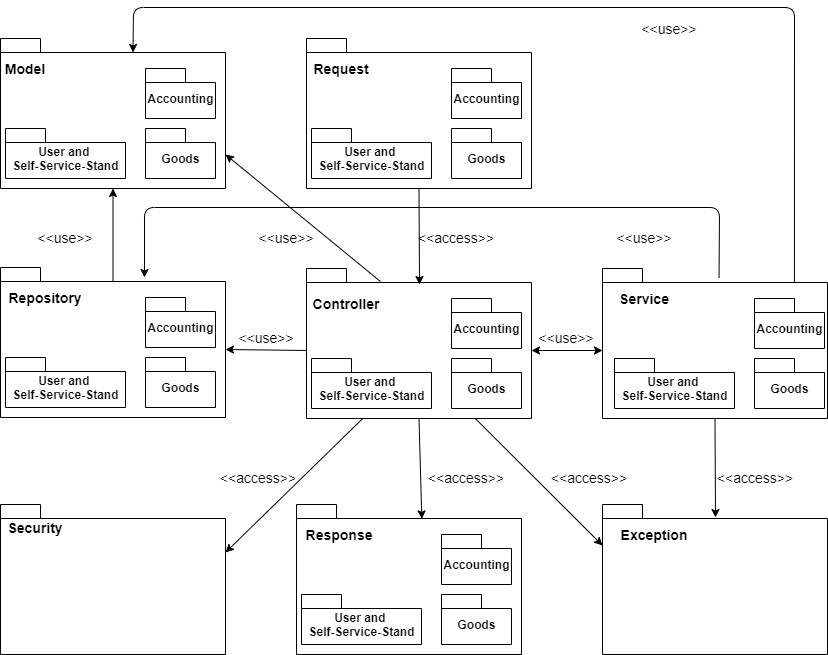
\includegraphics[width=1\textwidth,angle=0]{abb/Paketdiagramm}
	\caption[Paketdiagramm des Servers]{Paketdiagramm des Servers}
	\label{fig:AB_Paketdiagramm_Server}
\end{figure}


In der Abbildung ~\ref{fig:AB_Paketdiagramm_Server} ist das erstellte Paketdiagramm abgebildet, anhand des Paketdiagramms wird der Aufbau des Servers erläutert. 
\\
\\
Das Paket Request (Anfrage) enthält Klassen, die die Struktur der Anfragen an eine Schnittstelle festlegen. Beispielhaft enthält die Klasse Goods im Unterpaket goods unter anderem folgende Variablen goodsName, goodsPrice usw.. Sobald eine Anfrage an eine Schnittstelle gesendet wird, muss die vorgebende Struktur eingehalten werden. Das heißt zum Beispiel, gleiche Namen und vorgebende Datentypen (int, String usw.).
\\
Eines der wichtigsten Pakete ist das Controller Paket. Alle eingehenden Anfragen an die REST-API werden von einer Klasse im Paket Controller entgegengenommen. Der Controller entscheidet, was mit einer eingehenden Anfrage geschehen soll, zuerst prüft der Controller die eingehenden Daten auf Korrektheit. Anschließend steuert der Controller den Datenfluss und leitet die Daten weiter an die zuständigen Serviceklassen, Securityklassen oder Exeptionklassen.
\\
\\
Im Paket Response(Antwort) sind Klassen enthalten, die die Struktur der Ausgabennachrichten, die an einen Anfragenden zurückgesendet wird, festlegen.
\\
\\
Das Paket Service enthält Klassen und Methoden die die Anwendungslogik für den Controller bereitstellen. Im Unterpaket Good, werden z. B. Waren hinzufügen, geändert und gelöscht.
\\
\\
Sobald eine Exception (Ausnahme) ausgelöst wird, ist die zugehörige Klasse, die die Exceptions verwaltet, im Paket Exception zu finden sein. Exceptions werden von den Klassen in den Paketen Service und Controller ausgelöst. Eine Exception ist ein Programmfehler, der ohne Behandlung zu Abstürzen führen kann.
\\
\\
Verwaltet werden im Paket Repository Datenbankabfragen. Dieses kann z. B. eine Abfrage sein, ob eine bestimmte Ware bereits existiert oder die Suche nach einem Datensatz. Abfragen werden von Klassen aus den Paketen Service und Controller durchgeführt.
\\
\\
Im Paket Modell sind die Klassen vorhanden, die für die Datenbankmodellierung vonnöten sind. In diesen Klassen wird die Struktur der Datenbank abgebildet. Wie z. B. Primärschlüssel, Fremdschlüssel, Attribute und Datentypen.
\\
\\
Enthalten sind im Paket Security Klassen, die für die Sicherheit der Anwendung relevant sind.
\\
\\
Viele der dargestellten Pakete enthalten die drei Unterpakete Goods, User and Self-Service-Stand und Accounting in diesen sind die Klassen der entsprechenden Themen zusammengefasst.
\\
So enthält das Unterpaket Goods, Klassen die für die Verwaltung der Waren zuständig sind.
\\
Zusammengefasst werden die Benutzerklassen und Selbstbedienungsstandklassen, da sich einige Funktionen der Klassen in beiden Kategorien wiederfinden. 
\\
Zuletzt existiert noch das Unterpaket Accounting, hier finden sich Klassen, die für die Verwaltung, den Tagesabschluss usw. zuständig sind. 


\subsubsection{Entwurf der Rest-Schnittstellen}\label{entwurf_der_Schnittstellen}

Nachfolgend sind alle REST-API \ref{RestAPI} aufgeführt. Damit der HTTP-Client die Anfrage an die korrekte Schnittstelle senden kann, ist eine eindeutige Adressierung notwendig. 
\\
Anfragen werden an eine URL gesendet, z. B. an http://localhost:8080/role/, zusammen mit der HTTP-Anfragemethode (GET, POST usw.). In der nachfolgenden Aufzählung, ist der Übersichtlichkeit halber zuerst die HTTP-Anfragemethode und anschließend der URL Pfad angeben z. B. POST /endOfDay/.
\\
Die Datenübertragung via HTTP kann über den HttpBody oder über den HttpHeader erfolgen. Beispielhaft wird bei POST /goodsName/\{goodsName\} der Warenname über die URL übertragen.
\\
\\
\textbf{Schnittstelle Tagesabschluss(EndOfTheDayController)}
\\
Der EndOfTheDayController stellt die folgenden Schnittstellen zur Verfügung:
\begin{itemize}
	\itemsep0pt
	\item  POST /endOfDay/
	\item  PUT /endOfDay/
	\item  GET /endOfDay/
\end{itemize}

Diese Schnittstellen dienen zur Verwaltung des Tagesabschlusses, für jede Ware kann pro Tag nur eine Endabrechnung erstellt werden.\\
Die Schnittstelle POST/endOfDay/ sorgt dafür das ein neuer Eintrag erstellt werden kann.
\\
Mithilfe der Schnittstelle PUT/endOfDay/ kann dieser Eintrag editiert werden.\\
Die Schnittstelle GET/endOfDay/ übermittelt eine Auflistung, darin enthalten sind unter anderem die Angaben der theoretisch verkauften Waren und theoretische Einnahmen (ohne Diebstahl, beschädigte Ware usw.). 
%%%%%%%%%%%%%%%%%%%%%%%%%%%%%%%%%%%%%%%%%%%%%%%%%%%%%%%%%%%%%%%%%%%%%%%%%%%%%%%%%%%%%%%%%%%%%%%%%%%%%%%%%%%%%%%%%%%%%%%%%%%%%%%%%%%%%%%%%%%%%%%%%%%%%%%%%
\\
\\
\textbf{Schnittstelle Waren(GoodsController)}
\\
Der GoodsController stellt die folgenden Schnittstellen zur Verfügung:

\begin{itemize}
	\itemsep0pt
	\item  POST /goods/
	\item  PUT /goods/
	\item  DELETE /goods/
	\item  GET /goods/
	\item  GET /goods/\{selfServiceStandName\}
	\item  GET /goods/\{selfServiceStandName\}/\{goodsName\}
\end{itemize}

Mithilfe dieser Schnittstellen lassen sich neue Ware anlegen (POST/goods/), verändern (PUT/goods/), oder auch löschen (DELETE/goods/). Eine Ware kann nur gelöscht werden, wenn diese nicht genutzt wird. Die beiden Schnittstellen GET/goods/ geben eine Übersicht der Waren zurück, dieses kann eine Liste oder eine einzelne Ware sein.
%%%%%%%%%%%%%%%%%%%%%%%%%%%%%%%%%%%%%%%%%%%%%%%%%%%%%%%%%%%%%%%%%%%%%%%%%%%%%%%%%%%%%%%%%%%%%%%%%%%%%%%%%%%%%%%%%%%%%%%%%%%%%%%%%%%%%%%%%%%%%%%%%%%%%%%%%
\\
\\
\textbf{Schnittstelle Warenname(GoodsNameController)}
\\
Der GoodsNameController stellt die folgenden Schnittstellen zur Verfügung:

\begin{itemize}
	\itemsep0pt
	\item  POST /goodsName/\{goodsName\}
	\item  PUT /goodsName/
	\item  DELETE /goodsName/
	\item  GET /goodsName/
	
\end{itemize}

Die Schnittstellen der Klasse GoodsNameController enthalten Schnittstellen, die dafür verantwortlich sind, Warennamen hinzuzufügen (POST/goodsName/\{goodsName\}) zu ändern (PUT/goodsName/) und zu löschen (DELETE/goodsName/).\\ Außerdem kann eine Liste mit allen verfügbaren Namen ausgegeben werden.
Jeder Warenname kann nur einmalig vergeben werden. \\
Der Warennamen wird in einer separaten Tabelle gespeichert, dieses hat den Vorteil, dass Redundanzen vermieden werden. Außerdem wird so verhindert, das unterschiedliche Schreibweisen für ein und dieselbe Ware existieren.
%%%%%%%%%%%%%%%%%%%%%%%%%%%%%%%%%%%%%%%%%%%%%%%%%%%%%%%%%%%%%%%%%%%%%%%%%%%%%%%%%%%%%%%%%%%%%%%%%%%%%%%%%%%%%%%%%%%%%%%%%%%%%%%%%%%%%%%%%%%%%%%%%%%%%%%%%
\\
\\
\textbf{Schnittstelle Wareneingang(ReceiptController)}
\\
Der ReceiptController stellt die folgenden Schnittstellen zur Verfügung:

\begin{itemize}
	\itemsep0pt
	\item  POST /receipt/
	\item  PUT /receipt/
	\item  DELETE /receipt/\{receiptGoodsNr\}
	\item  GET /receipt/one\{receiptGoodsNr\}
	\item  GET /receipt/all/\{selfServiceStandName\}
	\item  GET /receipt/variety/\{selfServiceStandName\}/\{goodsName\}
\end{itemize}

Mithilfe dieser Schnittstellen wird der Wareneingang und Warenausgang protokolliert.\\
Mithilfe der Schnittstelle POST/receipt/ wird ein neuer Wareneingang oder Warenausgang hinzugefügt. PUT/receipt/ ändert diesen und DELETE/receipt/\{receiptGoodsNr\} löscht diesen Eintrag.\\
Die Schnittstelle GET/receipt/one/\{receiptGoodsNr\} übergibt einen einzelnen Datensatz. Eine Liste mit allen Eingängen und Ausgängen einer bestimmten Ware überliefert die Schnittstelle GET /receipt/variety/\{selfServiceStandName\}/\{goodsName\}.
\\
Die Schnittstelle GET/receipt/all/\{selfServiceStandName\} liefert ebenfalls eine Liste, mit allen Ein-und Ausgängen.
%%%%%%%%%%%%%%%%%%%%%%%%%%%%%%%%%%%%%%%%%%%%%%%%%%%%%%%%%%%%%%%%%%%%%%%%%%%%%%%%%%%%%%%%%%%%%%%%%%%%%%%%%%%%%%%%%%%%%%%%%%%%%%%%%%%%%%%%%%%%%%%%%%%%%%%%%
\\
\\
\textbf{Schnittstelle Benutzerrollen(RoleController)}
\\
Der RoleController stellt die folgenden Schnittstellen zur Verfügung:

\begin{itemize}
	\itemsep0pt
	\item  GET /role/
\end{itemize}

Die Schnittstelle GET/role/ gibt eine sortierte Liste mit allen verfügbaren Benutzerrollen zurück.
%%%%%%%%%%%%%%%%%%%%%%%%%%%%%%%%%%%%%%%%%%%%%%%%%%%%%%%%%%%%%%%%%%%%%%%%%%%%%%%%%%%%%%%%%%%%%%%
\\
\\
\textbf{Schnittstelle Selbstbedingungsstand (SelfServiceStandController)}
\\
Der SelfServiceStandController stellt die folgenden Schnittstellen zur Verfügung:

\begin{itemize}
	\itemsep0pt
	\item  POST /selfServiceStand/\{userName\}/\{selfServiceStandName\}
	\item  POST /selfServiceStand/addUser/
	\item  DELETE /selfServiceStand/\{removeUserName\}/\{userName\}/\{selfServiceStandName\}
	\item GET /selfServiceStand/\{selfServiceStandName\}
\end{itemize}


Diese Schnittstellen helfen bei der Verwaltung eines Selbstbedienungsstandes. Ein neuer Selbstbedienungsstand wird mit der Schnittstelle POST/selfServiceStand/\{userName\}/ \{selfServiceStandName\} erstellt, der Benutzer, der diesen erstellt hat, erhält Administratorrechte.
\\
Die Schnittstelle POST /selfServiceStand/addUser/ fügt einen bereits existierenden Benutzer einen Selbstbedienungsstand hinzu, dabei kann die Benutzerrolle frei gewählt werden. Sobald ein Benutzer entfernt werden soll, hilft die Schnittstelle DELETE/selfServiceStand/\{removeUserName\}/\{userName\}/\{selfServiceStandName\}.
\\
Eine Liste mit allen Benutzern, die dem Selbstbedienungsstand zugeordnet sind, wird mithilfe der Schnittstelle GET/selfServiceStand/\{selfServiceStandName\} ausgeben.
%%%%%%%%%%%%%%%%%%%%%%%%%%%%%%%%%%%%%%%%%%%%%%%%%%%%%%%%%%%%%%%%%%%%%%%%%%%%%%%%%%%%%%%%%%%%%%%%%%%%%%%%%%%%%%%%%%%%%%%%%%%%%%%%%%%%%%%%%%%%%%%%%%%%%%%%%
\\
\\
\textbf{Schnittstelle Einheiten(UnitController)}
\\
Der UnitController stellt die folgenden Schnittstellen zur Verfügung:

\begin{itemize}
	\itemsep0pt
	\item  POST /unit/\{unitName\}
	\item  PUT /unit/\{oldUnitName\}/\{newUnitName\}
	\item  DELETE /unit/\{unitName\}
	\item  GET /unit/\{unitName\}
\end{itemize}
Einheiten wie z. B. Stück KG, Sack usw. können mit der Schnittstelle POST/unit/ erstellt werden. Verändert werden können diese mit der Schnittstelle PUT /unit/\{oldUnitName\}/\{newUnitName\}. Soll eine Einheit gelöscht werden, ist dieses mit der Schnittstelle DELETE/unit/\{unitName\} möglich.
\\ Allerdings können Änderung und Löschungen nur durchgeführt werden, wenn die Einheit noch nicht verwendet wird.
Eine Liste der verfügbaren Einheiten gibt die Schnittstelle GET/unit/\{unitName\} aus.
%%%%%%%%%%%%%%%%%%%%%%%%%%%%%%%%%%%%%%%%%%%%%%%%%%%%%%%%%%%%%%%%%%%%%%%%%%%%%%%%%%%%%%%%%%%%%%%%%%%%%%%%%%%%%%%%%%%%%%%%%%%%%%%%%%%%%%%%%%%%%%%%%%%%%%%%%
\\
\\
\textbf{Schnittstelle Benutzer(UserController)}
\\
Der UserController stellt die folgenden Schnittstellen zur Verfügung:

\begin{itemize}
	\itemsep0pt
	\item  POST /user/newAdmin
	\item  POST /user/newUser
	\item  PUT /user/
	\item  GET /user/\{username\}
\end{itemize}

Die Benutzerverwaltung kann mithilfe nachfolgender Schnittstellen durchgeführt werden. Ein neuer Benutzer und ein neuer Selbstbedienungsstand werden mit der Schnittstelle POST/user/newAdmin erstellt. Der neu erstellte Benutzer wird automatisch dem erstellten Selbstbedienungsstand als Administrator zugeordnet. Der Name des Selbstbedienungsstandes und des Benutzers darf noch nicht vergeben sein.
\\
Ein Administrator eines Selbstbedienungsstandes kann einen neuen Benutzer zu diesem hinzufügen, der Benutzer wird dabei neu erstellt, die Benutzerrolle kann frei gewählt werden, dieses geschieht mit der Schnittstelle POST/user/newUser.
\\
Sobald ein neuer Benutzer erstellt wird, wird zuerst überprüft, ob der Benutzername bereits vergeben ist, sollte dieses der Fall sein, kann der Benutzer nicht erstellt werden. Die Schnittstelle PUT/user/ ist zum Editieren des Benutzers gedacht. Ein einzelner Benutzer kann mit der Schnittstelle GET/user/\{username\} ausgegeben werden.

\subsection{Entwurf des Clients}\label{entwurf_des_Clients}

Im nachfolgenden Kapitel wird genauer auf den Entwurf des Clients eingegangen. Das Kapitel wird unterteilt in Entwurf der grafischen Benutzeroberfläche und Entwurf des Hintergrundbereiches.

\subsubsection{Entwurf der grafischen Benutzeroberfläche (Frontend)}\label{entwurf_der_grafischen_Benutzeroberfläche_(Frontend)}
Die Zielsetzung bei der Oberflächengestaltung dieser Anwendung ist, dass diese möglichst übersichtlich und schlicht gestaltet sein soll.
\\
\cite{gui} nennt Tipps zur Gestaltung, unter anderem \grqq Reduziere auf das Wesentliche\grqq{} es sollen nur die nötigsten und wichtigsten Informationen und Schaltflächen dargestellt werden.
\\
Die Anwendung soll nur zwei Hauptbereiche umfassen, das sind der Anmeldebildschirm und das Hauptmenü. Auf diese wird nachfolgend kurz eingegangen. 

\begin{figure}[htb]
	\centering
	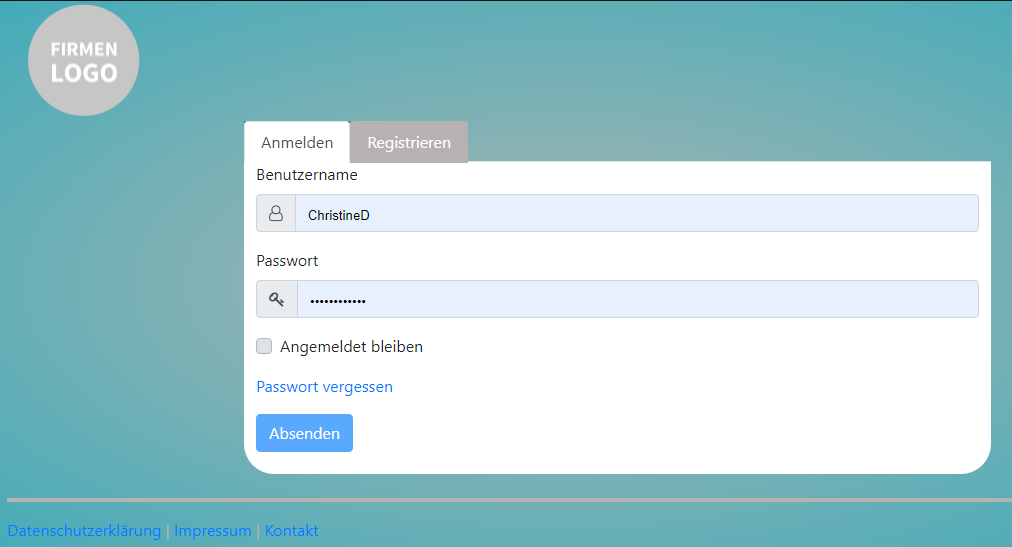
\includegraphics[width=1\textwidth,angle=0]{abb/login}
	\caption[Anmeldebildschirm]{Anmeldebildschirm}
	\label{fig:Anmeldebildschirm}
\end{figure}

Die~\ref{fig:Anmeldebildschirm} Abbildung zeigt den Anmeldebildschirm, dort können sich die Benutzer Anmelden und Registrieren.
\\
Ein weiterer Tipp von \cite{gui} wird hier umgesetzt, dieser heißt \glqq Orientiere dich an bereits erstellten Oberflächen\grqq{}. Vielen Anwendern ist die Struktur des Anmeldebildschirmes bereits von anderen Anwendungen bekannt, dadurch fällt Ihnen die Bedienung leichter, da sie vieles wiedererkennen.
\\
Sobald der JSON Web Token ungültig ist oder abgelaufen, wird der Nutzer immer auf den Anmeldebildschirm umgeleitet. Ein Token dient zur gegenseitigen Authentifizierung von Client und Server, erklärt \cite{token}. Sobald ein Benutzer sich zum ersten mal anmeldet, wird eine Anfrage (Request) an den Server gestellt. Dieser sendet eine Antwort (Response) zurück, sind die Anmeldedaten gültig, wird zusätzlich der Token mitgesendet. Der Token wird bei jeder erneuten Kommunikation mit dem Server mitgesendet.

\begin{figure}[htb]
	\centering
	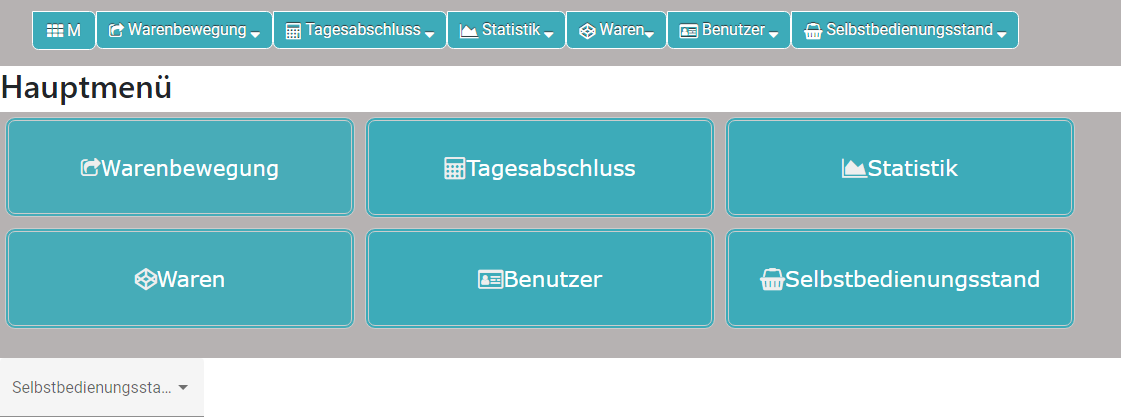
\includegraphics[width=1\textwidth,angle=0]{abb/hauptm}
	\caption[Hauptmenü]{Hauptmenü}
	\label{fig:Hauptmenü}
\end{figure}

Die Abbildung~\ref{fig:Hauptmenü} stellt das Hauptmenü da. Im oberen Bereich ist eine Navigationsleiste abgebildet, diese wird dauerhaft angezeigt. Der mittlere Bereich wird je nach Bedarf ausgetauscht. Im unteren Sektor kann der Anwender zwischen bestehenden Selbstbedienungsständen wechseln. 
\\
\\
Sobald der Nutzer den Punkt Warenbewegung auswählt, kann er dort die Warenbewegungen (Eingänge und Ausgänge) und das Datum eintragen.
\\
Ein Tagesabschluss wird erstellt, sobald der Anwender auf Tagesabschluss geht.
\\
Unter dem Menüpunkt Statistik sind Monats- und Jahresstatistiken zu finden.
\\
Mithilfe der Menüpunkte Waren, Benutzer und Selbstbedienungsstand können Waren, Benutzer und der Selbstbedienungsstand geändert, gelöscht oder hinzugefügt werden. 


\subsubsection{Entwurf des Hintergrundbereiches (Backend)}\label{entwurf_des_Hintergrundbereiches_(Backend)}

Die Ausgangsidee ist, die angefertigt Skizze des Hauptmenüs und des Anmeldebildschirmes, aus dem vorigen Kapitel, in einzelne Bestandteile bzw. Komponenten zu zerlegen.\\
 Die Abbildung ~\ref{fig:kompo} stellt dieses dar. 

\begin{figure}[htb]
	\centering
	\includegraphics[width=1\textwidth,angle=0]{abb/kompo}
	\caption[Darstellung der Komponenten des Clients]{Darstellung der Komponenten des Clients}
	\label{fig:kompo}
\end{figure}

Zu sehen ist der Hauptbereich~\ref{fig:kompo} unterteilt in einzelne Komponenten die jeweils farbig dargestellt sind. Die grün dargestellten Komponenten werden dauerhaft eingeblendet, dieses sind der Fußbereich, Hauptmenü und Auswahl des Selbstbedienungsstandes. 
\\
\\
Je nachdem in welchem Menü der Anwender sich befindet, wird im Hauptbereich (Gelb) situationsabhängig unterschiedliche Unterpunkte (Orange) angezeigt. Je nachdem, was der Benutzer davon auswählt, wird dieses im Hauptbereich eingeblendet.
\\
Dadurch ergibt sich folgende Struktur.
\begin{itemize}
	\itemsep0pt
	\item Hauptmenü
	\item Hauptbereich
		\subitem - Tagesabschluss 
			\subsubitem + Eintrag bearbeiten oder anlegen
			\subsubitem + Übersicht Tagesabschluss
		\subitem - Warenverwaltung 
			\subsubitem + Ware anlegen oder ändern
			\subsubitem + Übersicht Warenverwaltung
		\subitem - Warenbewegung 
			\subsubitem + Warenbewegung hinzufügen
			\subsubitem + Übersicht Warenverwaltung
			\subsubitem + Warenoptionen
		\subitem - Benutzerverwaltung 
			\subsubitem + Benutzerdaten bearbeiten
			\subsubitem + Übersicht Warenverwaltung
		\subitem - Selbstbedienungsstandverwaltung 
				\subsubitem + Selbstbedienungsstanddaten bearbeiten
				\subsubitem + Benutzer zum Selbstbedienungsstand hinzufügen
				\subsubitem + Benutzer anlegen und Selbstbedienungsstand hinzufügen
		\subitem - Statistik 
				\subsubitem + Monatsstatistik anzeigen
				\subsubitem + Jahresstatistik anzeigen
	\item Fußbereich
	\item Auswahl des Selbstbedienungsstandes
	
\end{itemize}


Zusätzlich werden unterschiedliche Serviceklassen angelegt, diese beinhalten Inhalte die von mehren unterschiedlichen Komponenten genutzt werden. 



\newpage

\section{Realisierung und Implementierung}\label{realisierungundImplementierung}

Diese Kapitel thematisiert die Realisierung und Implementierung. Zunächst wird die Implementierung der SQL-Datenbank vorgestellt, danach folgt die Implementierung des Servers und des Clients. Es werden jeweils ein paar Quellcodeausschnitte näher beleuchtet.

\subsection{Implementierung der SQL Datenbank}

Zuerst wird XAMPP\footnote{https://www.apachefriends.org/de/index.html} heruntergeladen, installiert und eingerichtet. 
\cite{DB5} schreib das XAMPP nur eine lokale Testumgebung simuliert, XAMPP sollte mit der Grundkonfiguration nicht als Webserver im Internet eingesetzt werden, da es Sicherheitslücken aufweist. XAMPP bündelt unterschiedliche freie Software, darunter auch einen lokalen Webserver mit der Datenbank MariaDB und phpMyAdmin.
\\
Im Anschluss wird eine Datenbank für das Projekt mit dem Namen db\_SB\_V1 angelegt.
\\
\\
Anschließend umgesetzt und realisiert werden die entworfenen Tabellen aus dem Kapitel ~\ref{normalisierung}.
Im Zug des Implementierungsprozesses, werden die Tabellen- und Spaltennamen ins Englische übertragen. Folgendes Schema zur Namensgebung wird verwendet.
\begin{itemize}
	\itemsep0pt
	\item Datenbankname: db\_Datenbankname
	\item Tabellenname: tb\_Tabellenname
	\item Spaltenname: cl\_Spaltenname
\end{itemize}
Beispielhaft wird nachfolgend die Tabelle~\ref{3NF Tagesabschluss} implementiert. 



\lstset{language=SQL}
\begin{lstlisting}[frame=htrbl, caption={Erstellung der Tabelle tb\_end of-the-day mit Hilfe des SQL-Behelfes CREATE}, label={lst:tbWaren}]	
CREATE TABLE `tb_end of-the-day` (
	`cl_graduation-date` date NOT NULL,
	`cl_goods-nr` int(10) UNSIGNED NOT NULL,
	`cl_user-nr` int(10) UNSIGNED NOT NULL,
	`cl_graduation-count` int(10) UNSIGNED NOT NULL,
	`cl_graduation-sold` int(10) UNSIGNED NOT NULL,
	`cl_graduation-revenue` decimal(6,2) UNSIGNED NOT NULL
) ENGINE=InnoDB DEFAULT CHARSET=utf8mb4;

\end{lstlisting}	

In Listing~\ref{lst:tbWaren} ist zu sehen wie mithilfe des Befehls CREATE eine neue Tabelle mit den Namen tb\_end of-the-day angelegt wird. 
\\
Folgende Datentypen werden eingesetzt, int (Zahl, von -2.147.483.648 bis 2.147.483.647), VARCHAR (Zeichenkette, bis zu 65.535 Zeichen), decimal (Vorkommastelle Anzahl, Nachkommastelle Anzahl)und DATE (Datum, im Format YYYY-MM-DD).
\\
Durch die Option NOT NULL wird sichergestellt, dass bei Erstellung eines neuen Tupels das Feld einen Wert hat.
Die Option UNSIGNED sorgt dafür, das kein Vorzeichen (+,-) eingeben werden kann, diese hat den Vorteil das nur positive Zeichen eingeben werden können.



\lstset{language=SQL}
\begin{lstlisting}[frame=htrbl, caption={Veränderung der Tabelle tb\_receiptgoods mit Hilfe des SQL-Behelfes ALTER}, label={lst:tbWarenZ}]
ALTER TABLE `tb_end of-the-day`
ADD PRIMARY KEY (`cl_graduation-date`,`cl_goods-nr`),
ADD KEY `cl_goods-nr` (`cl_goods-nr`),
ADD KEY `cl_user-nr` (`cl_user-nr`);


ALTER TABLE `tb_end of-the-day`
ADD CONSTRAINT `tb_end of-the-day_ibfk_1` 
FOREIGN KEY (`cl_goods-nr`) REFERENCES `tb_goods` (`cl_goods-nr`),
ADD CONSTRAINT `tb_end of-the-day_ibfk_2` 
FOREIGN KEY (`cl_user-nr`) REFERENCES `tb_user` (`cl_user-nr`);
			
\end{lstlisting}	


Mit der Anweisung ALTER TABLE können nachträglich unter anderem Optionen hinzugefügt werden, zu sehen ist dieses in Listing \ref{lst:tbWarenZ}. Es wird ein zusammengesetzter Primärschlüssel festgelegt mit der Option ADD PRIMARY KEY, die beiden Spalten cl\_graduation-date und cl\_goods-nr bilden das Schlüsselpaar.
\\
Anschließend wird die Anweisung ALTER TABLE erneut durchgeführt, es wird ein Fremdschlüssel (FOREIGN KEY) für die Spalten cl\_goods-nr und cl\_user-nr generiert. 
In diesem Beispiel, werden die Spalte cl\_goods-nr mit einem Datensatz in der Tabelle tb\_goods, Spalte cl\_goods-nr verknüpft.
\\
\\
\newpage

\begin{figure}[htb]
	\centering
	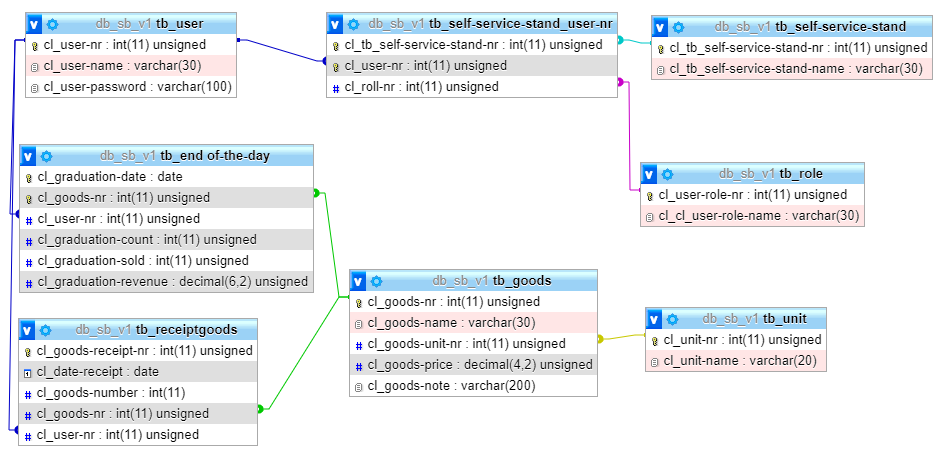
\includegraphics[width=1\textwidth,angle=0]{abb/erstellteTabellen}
	\caption[Übersicht, erstellte Tabellen]{Übersicht, erstellte Tabellen}
	\label{fig:erstellteTabellen}
\end{figure}

Die Abbildung~\ref{fig:erstellteTabellen} stellt die erstellten Tabellen grafisch dar. Aus der Abbildung lassen sich die einzelnen Tabellen, mit den Spalten und den verwendeten Datentypen ablesen. Außerdem können die Primärschlüssel, erkennbar am gelben Schlüssel, leicht identifiziert werden.
Die genutzten Fremdschlüssel lassen sich ebenfalls erkennen, dargestellt durch die farbigen Verbindungslinien.


\subsubsection{MariaDB und phpMyAdmin}\label{MariaDB und phpMyAdmin}
MariaDB ist ein bekanntestes Datenbankmanagementsystem (DBMS), dieses wird in diesem Projekt genutzt. In diesem Kapitel wird erläutert, warum dieses System verwendet wird.
\\

MariaDB\footnote{https://mariadb.com} wurde im Jahr 2009 veröffentlicht. Das DBMS unterliegt einer GPL2 Open-Source Lizenz, das heißt sowohl private als auch kommerzielle Nutzung ist erlaubt. Entwickelt wurde MariaDB von Michael Widenius, er entwickelte ebenfalls MySQL, aus diesem Grund gibt es sehr viele Gemeinsamkeiten. 
\\
MariaDB hat eine gute Geschwindigkeit und Performance, bei der Durchführung von Datenbankabfragen. Die Seite \cite{DB4} schreibt \grqq Features wie Hochverfügbarkeit, Security, Interoperabilität und Performanceverbesserungen aufweist.\grqq{} bietet MariaDB. 
\\
Damit die Verwaltung der Datenbank komfortabler ist, wird die Software phpMyAdmin\footnote{https://www.phpmyadmin.net} verwendet. PhpMyAdmin ist weitverbreitet und die Standartsoftware zum Verwalten von Datenbanken. 

\subsection{Implementierung des Spring Boot Servers}

Für die Entwicklung des Servers wurde Spring Boot gewählt. Spring Boot ist eine Open Source Software und kann kostenlos genutzt werden. Außerdem existiert eine große Community, die bei Fragen weiterhelfen kann. Spring Boot bietet außerdem einen großen Funktionsumfang. Es lassen sich leicht neue Funktionen usw. integrieren. Allerdings erfordert Spring Boot etwas Einarbeitungszeit.
 \\
 \\
Nachfolgend werden einige Quellcodeausschnitte etwas genauer erläutert. Der komplette Quellcode der Klasse ist im Anhang \ref{QuellcodeServer} zu finden.
Zuerst werden zwei Klassen aus dem Paket model dargestellt, anschließend werden aus den Paketen controller, service und repoitory ebenfalls Klassen vorgestellt. 
\\
\\
Um die objektrelationale Abbildung der Datenbank zu erleichtern, wird JPA(Java Persistence API) verwendet, JPA ist im Spring Boot Framework enthalten. \cite{JPA} schreibt \grqq Die Java Persistence API (JPA) des Java Community Process ist ein Standard für das Objekt-relationale Mapping (ORM) von Java-Objekten. ORM ist ein Verfahren zur Speicherung von Objekten in Datenbanken - Klassen und Objekte werden auf Tabellen und Zeilen abgebildet.\grqq{}. 

\subsubsection{Beispielcodeausschnitte aus Model-Klassen}

Die Klasse EndOfTheDay \ref{lst:EndOfTheDay} befindet sich im Paket model, die Klasse bildet die Datenbankstruktur der Tabelle tb\_end of\_the\_day ab. Die Datenbanktabelle enthält unter anderem einen zusammengesetzten Primärschlüssel, sowie drei Fremdschlüssel. 
\\
\lstset{language=java}
\begin{lstlisting}[frame=tb, caption={Das Listing zeigt einen Ausschnitt aus der Klasse EndOfTheDay}, label={lst:EndOfTheDayAus}]
@Table(name = "tb_end of_the_day", indexes = {
	@Index(name = "cl_user_nr", columnList = "cl_user_nr"),
	@Index(name = "cl_goods_nr", columnList = "cl_goods_nr"),
	@Index(name = "cl_self_service_stand_nr", columnList = "cl_self_service_stand_nr")
})
@Setter
@Getter
@Entity
public class EndOfTheDay {
	
	/**
	* ID End of the Day.
	*/
	@EmbeddedId
	private EndOfTheDayId id;
	
	/**
	* Refers to a user ID.
	*/
	@ManyToOne
	@JoinColumn(name = "cl_user_nr", nullable = false)
	private User userNr;
\end{lstlisting}

Im Codeausschnitt \ref{lst:EndOfTheDayAus} Zeile 1, ist die Zuordnung einer bereits bestehenden Tabelle in einer Datenbank mithilfe der JPA-Annotationen @Table zu sehen. Anschließend wird in den Zeilen 2 bis 5 die Fremdschlüsselverknüpfung durchgeführt, dabei wird auf eine Spalte in einer anderen Tabelle verwiesen.
\\
\\
Die Annotationen @Setter und @Getter in Zeile 6 und 7 sorgen dafür, das die Getter und Setter Methoden nicht mehr implementiert werden müssen. Sondern mithilfe des Java-Framework Lombok automatisch intrigiert werden.
\\
\\
Die JPA-Annotationen @Entity in der 8 Zeile bewirkt das automatisch alle Attribute in der Klasse auf gleichnamige Datenbankspalten (Mapping) abgebildet werden. Es kann der Fall auftreten, dass die Attribute und Spaltennamen unterschiedlich heißen, wie z. B. in Zeile 22 Mit der Annotation @JoinColumn(name = \grqq{}cl\_user\_nr\grqq{}) in Zeile 21 wird der Tabellenspaltname zugewiesen.
\\
\\
Da es sich bei dem Attribute User um eine Fremdschlüsselverknüpfung handelt, wird in Zeile 20 eine 1:n Beziehung hinzugefügt, es wird ein User-Objekt deklariert.
\\
\\
Bei der ID handelt es sich um einen zusammengesetzten Primärschlüssel, siehe Zeile 13 und 19. Es wird ein EndOfTheDayId-Objekt erstellt. Im Listing \ref{lst:EndOfTheDayIdAus} ein Codeausschnitt der Klasse EndOfTheDayId abgebildet. In Zeile 8 und 14 sind die Attribute zu sehen aus denen sich der zusammengesetzte Primärschlüssel definiert. Die Annotationen in Zeile 1 deutet darauf hin, dass in dieser Klasse ein zusammengesetzter Primärschlüssel vorhanden ist.
\\
\lstset{language=java}
\begin{lstlisting}[frame=tb, caption={Das Listing zeigt einen Ausschnitt aus der Klasse EndOfTheDayId}, label={lst:EndOfTheDayIdAus}]
@Embeddable
public class EndOfTheDayId implements Serializable {
	
	/**
	* serialVersionUID
	*/
	private static final long serialVersionUID = 4548732131340178144L;
	
	/**
	* End of the day date.
	*/
	@Column(name = "cl_graduation_date", nullable = false)
	private LocalDate graduationDate;
	
	/**
	* The commodity number.
	*/
	@Column(name = "cl_goods_nr", nullable = false)
	private Integer goodsNr;
\end{lstlisting}

\subsubsection{Beispielcodeausschnitte aus Repository-Interfaces}

Im Paket repository sind Interfaces enthalten, die für Datenbankoperationen zuständig sind. Es handelt sich nicht um Standard JPA, sondern es wird Spring Data JPA verwendet. Genutzt wird die Kurzschreibweise für Abfragen.

\lstset{language=java}
\begin{lstlisting}[frame=tb, caption={Das Listing zeigt einen Ausschnitt aus dem Interface GoodsNameRepository}, label={lst:GoodsNameRepositoryAus}]
@Repository
public interface GoodsNameRepository extends JpaRepository<GoodsName, Integer> {
	
	//Query list of all goods names, sorted by unit name.
	List<GoodsName> findByOrderByGoodsNameAsc();
	
	//Query, goods name with the name exists.
	boolean existsByGoodsNameIs(String goodsName);
	
}
\end{lstlisting}

Im Listing \ref{lst:GoodsNameRepositoryAus} ist das Repository des Interfaces GoodsNameRepository abbildet. Das Interface erbt vom Interface JpaRepository Zeile 2. \\
In der Zeile 5 ist eine Datenbankabfrage zu sehen die eine sortierte Liste mit allen vorhanden Einträgen in der Tabelle zurückliefert. 
\\
Eine weitere Abfrage ist in Zeile 8, diese Abfrage liefert ein True zurück, sobald ein Eintrag mit der eingebenden Zeichenkette übereinstimmt. 
\\
\lstset{language=java}
\begin{lstlisting}[frame=tb, caption={Das Listing zeigt einen Ausschnitt aus dem Interface ReceiptGoodRepository}, label={lst:ReceiptGoodRepositoryAus}]
List<ReceiptGoods> findByDateReceiptAndGoodsNr_GoodsId(LocalDate dateReceipt, Integer goodsId);
\end{lstlisting}

Das Listing \ref{lst:ReceiptGoodRepositoryAus} liefert ein Beispiel für eine Verknüpfte Und-Abfrage. Außerdem wird in der Tabelle nach einem Fremdschlüsseltribut (GoodsNr\_GoodsId) gesucht.

\subsubsection{Beispielcodeausschnitte aus einer Controller-Klasse}


\lstset{language=java}
\begin{lstlisting}[frame=tb, caption={Das Listing zeigt einen Ausschnitt aus der Klasse unitController}, label={lst:unitControllerAus}]
@RestController
@RequestMapping("/unit")
public class UnitController {
		
	/**
	* unitRepository to handle unit information.
	*/
	private final UnitRepository unitRepository;
	
	/**
	* goodsRepository to handle goods information.
	*/
	private final GoodsRepository goodsRepository;
	
	/**
	* Service to handle self-service stand information logic.
	*/
	private final UnitService unitService;
	
	public UnitController(UnitRepository unitRepository, GoodsRepository goodsRepository, UnitService unitService) {
		this.unitRepository = unitRepository;
		this.goodsRepository = goodsRepository;
		this.unitService = unitService;
	}
\end{lstlisting}

In Zeile 1 wird festgelegt, dass es sich bei der Klasse um einen Rest-Controller handelt. 
\\
Mapping wird in der 2. Zeile durchgeführt.\cite{mapping} beschreibt, das es beim Mapping \glqq um die Konversion von zwei verschiedenen Adressräumen.\glqq{} geht.\glqq Dabei werden die Daten eines Adressraums auf einen zweiten Adressraum abgebildet.\glqq{}
\\
Alle Klassen mit der Annotation @Repository, @Controller, @Service oder @Component werden automatisch als Bean erkannt und registriert. In der Spring Dokumentation \cite{spring} steht das ein Bean, ein Objekt ist, das von einem Spring IoC-Container instanziiert, assembliert und verwaltet wird.
\\
\\
Es wird das Endwurstmuster Dependency Injektion verwendet. Dieses besagt, das Komponenten und Klassen soweit möglich unabhängig von anderen Klassen sein sollen, bekannt auch als lose Kopplung, erklärt \cite{Dependency}.  \grqq Als Dependency Injection bezeichnet man in der objektorientierten Programmierung eine externe Instanz, die die Abhängigkeiten von Objekten im Vorhinein regelt \grqq{} \cite{Spring1}.
\\
In diesem Projekt wird mithilfe von Constructor-Injection (Konstruktor-Injektion) das Objekt injiziert. Dieses ist in den Zeilen 8 bis 24 zu erkennen, es werden sowohl Repositoryklassen und eine Serviceklasse eingebunden, Zeilen 8 bis 18. Diese werden im Konstruktor injizierten, Zeile 20 bis 24.
\\
\lstset{language=java}
\begin{lstlisting}[frame=tb, caption={Das Listing zeigt eine Methode aus der Klasse unitController}, label={lst:unitControllerAusM}]
/**
* Method returns a sorted list with all units.
*
* @return json list with all units
*/
@GetMapping(path = "/", produces = MediaType.APPLICATION_JSON_VALUE)
    private ResponseEntity<List<Unit>> getUnits() {
	
	//Return sorted list, sorted by unit name.
	return new ResponseEntity<>(unitService.getUnitsList(), HttpStatus.OK);
}
\end{lstlisting}

Im Listing \ref{lst:unitControllerAusM} ist eine Methode aus der Klasse UnitController abgebildet. Diese Methode wird durch die REST-Schnittstelle GET /unit angesprochen (\ref{lst:unitControllerAus}). Der Pfad /unit wurde bereits am Klassenanfang festgelegt \ref{lst:unitControllerAus} Zeile 1. Da in dieser Klasse nur eine Get-Schnittstelle angesprochen wird, kann diese eindeutig infiziert werden, eine weitere Pfad Angabe ist nicht nötig. 
\\
Die Methode gibt eine Json-Liste und einen HttpStatus zurück. Diese ist in Zeile 10 implementiert. Außerdem ist zu sehen, wie eine Service Bean aufgerufen wird, (unitService.getUnitsList()). Dadurch wird die entsprechende Methode in der Serviceklasse ausgelöst.














\subsection{Implementierung des Angular-Clients}

Diese Kapitel erläuterte die Implementierung des Angular-Clients. Zuerst wird auf die Implementierung der grafischen Benutzeroberfläche eingegangen. Danach folgt die Implementierung des Hintergrundbereiches.


\subsubsection{Implementierung der grafischen Benutzeroberfläche (Frontend)}

In diesem Kapitel wird auf die Implementierung der grafischen Benutzeroberfläche eingegangen, nachfolgend werden einige Quellcodeausschnitte gezeigt. Zuerst wird kurz auf das Grid Layout eingegangen.
\\
\\
\newpage
Eines der Hauptmerkmale von Angular ist, das dieses komponentenbasiert arbeitet. 
Da bereits bei der Konzeption die Oberflächen in Komponenten eingeteilt worden sind, bietet es sich an, Angular zu verwenden.
\\
\\
Jede dieser Komponenten enthält eine CSS-Datei, HTML-Datei und eine Typscript-Datei. In diesem Kapitel wird auf die CSS-Datei und HTML-Datei eingegangen.
\\
\\
Das Gestaltungsraster wird mithilfe CSS Grid Layout gestaltet. Mithilfe von Grid lässt sich eine Seite in einzelne Raster aufteilen, die Flächen müssen nicht die gleiche Größe haben, sondern nur rechteckig sein. 
Die Komponenten werden den Rasterzellen zugewiesen.

\lstset{language=html}
\begin{lstlisting}[frame=tb, caption={Umsetzung des Grid-Layout}, label={lst:grid}]
.container {
	display: grid;
	grid-template-columns: 0.5fr 2fr 8fr 2fr 0.5fr;
	grid-template-rows: 0.4fr 3.4fr 0.4fr 0.4fr;
	gap: 0px 0px;
	grid-auto-flow: row;
	grid-template-areas:
	"navbar navbar navbar navbar navbar"
	"main main main main main"
	"selectSelf selectSelf . . ."
	"footer footer footer footer footer";
}

.navbar {
	grid-area: navbar;
	background: var(--colorGray);
}
	\end{lstlisting}


Im Listing~\ref{lst:grid} ist ein Ausschnitt aus einer CSS-Datei zusehen. In dieser, wird die Vorlage aus dem Kapitel 4 Entwurf der grafischen Benutzeroberfläche ~\ref{fig:Hauptmenü} mit Grid umgesetzt.
\\
In den Zeilen 3 und 4 ist zu sehen, wie Größe und Anzahl der Spalten und Zeilen festgelegt wird, es gibt fünf Spalten und vier Zeilen. In Zeile 7 bis 11 werden den Rasterbereichen Namen zugewiesen, der Bereich navbar (Hauptmenü) ist beispielsweise in Zeile eines, Spalte zwei bis vier zu finden.
 \\
Die Zeilen 14 bis 17 zeigen, wie einer CSS-Klasse der Grid-Bereich navbar zugewiesen wird. In Zeile 16 wird die Farbe des Hintergrundbereiches festgelegt, die Farbe ist in einer Variabel gespeichert. Dieses hat den Vorteil, dass die festgelegt Farbe schnell und leicht änderbar ist.
\\


\lstset{language=html}
\begin{lstlisting}[frame=tb, caption={Zuweisung der Komponenten in HTML}, label={lst:html}]
<div class="container">
	<div class="navbar">
		<app-navbar></app-navbar>
	</div>
	<div class="main">
		<router-outlet></router-outlet>
	</div>
	<div class="footer">
		<app-footer></app-footer>
	</div>
\end{lstlisting}

Im Listing~\ref{lst:grid} ist ein Teilausschnitt einer HTML-Datei abgebildet.
Das Listing~\ref{lst:html} veranschaulicht die Zuweisung der CSS-Klassen z. B. in Zeile 2.
\\
Außerdem ist zu sehen wie erstellte Angular-Komponenten eingebunden werden, Zeile 3 und 9.
\\
In Zeile 6 wird das Router-Outlet im Hauptbereich implementiert. Angular sorgt automatisch dafür dass die richtige Komponente eingefügt wird. Mithilfe von vordefinierten internen Routinezuweisungen wird die passende Komponente ausgewählt. Mehr dazu im nachfolgenden Kapitel.
\\

\lstset{language=html}
\begin{lstlisting}[frame=tb, caption={Schleifen und Abfragen in HTML}, label={lst:html1}]
<tr (click)="setValues(goods.goodsId)" *ngFor="let goods of searchResultList">
	<td>{{goods.goodsId}}</td>
	<td>{{goods.goodsName}}</td>
	<td>{{goods.unitName}}</td>
	<td>{{goods.goodsPrice}}</td>
	<td>{{goods.goodsNote}}</td>
	<div *ngIf=goods.goodsActive>
		<td>Ja</td>
	</div>
	<div *ngIf=!goods.goodsActive>
		<td>Nein</td>
	</div>
</tr>
\end{lstlisting}

Im Listing~\ref{lst:html1} ist eine forEach-Schleife und zwei IF-Abfragen zu sehen. 
Die forEach-Schleife befindet sich in der Zeile 1,(*ngFor=\grqq{}let goods of searchResultList) es wird eine Liste (searchResultList), diese wurde in der dazugehörigen TypeScript-Datei initialisiert, durchlaufen. Der nachfolgende HTML-Code wird dabei so oft ausgeführt wie es der Länge der Liste entspricht. Für jeden Schleifendurchlauf wird ein Element in die Variabel goods gespeichert. Diese wird nachfolgende ausgeben. 
\\
In Zeile 7 wird eine If-Abfrage durchgeführt, dabei wird überprüft, ob goods.goodsActive mit dem Wert True initialisiert worden ist. Ist dieses der Fall werden alle Elemente im nachfolgenden Div-Element ausgeführt.

\subsubsection{Implementierung des Hintergrundbereichs (Backend)}

Es werden in diesem Kapitel einige TypeScript-Quellcodeausschnitte gezeigt.

\lstset{language=java}
\begin{lstlisting}[frame=tb, caption={Festlegung der internen Routen in Angular}, label={lst:html2}]
const myRoutes: Routes = [
{
	path: '',
	component: MainScreenComponent,
	children: [
	{
		path: 'goods',
		component: GoodsComponent,
		children: [
		{
			path: 'overview',
			component: OverviewGoodsComponent
		},
		{
			path: 'new',
			component: NewGoodsComponent
		},
		{
			path: 'change',
			component: ChangeGoodsComponent
		}, {
			path: 'settings',
			component: SettingsGoodsComponent
		}
		]
	},	
\end{lstlisting}

Im ersten Listing~\ref{lst:html2} dieses Kapitels ist zu sehen, wie die internen Routen in der Konstante myRoutes gespeichert werden, Zeile 1. Mithilfe von internen Routen ist es möglich innerhalb von Angular zu navigieren oder die Ansichten zu ändern. Dieses wird im Quellcode Listing \ref{lst:html1} Zeile 6 genutzt. 
\\
Im Listing \ref{lst:html3} ist HTML-Code abgebildet, in der Zeile 4 ist ein interner Link zu sehen, dieser leitet weiter zum Pfad /goods/overview. Es können Eltern-Pfad-Routen und deren Kinderelemente festgelegt werden, dargestellt im Listing~\ref{lst:html2} Zeile 5 bis 26.
\\
Dass RouterModule welches importiert wird, übernimmt das Routing für den Entwickler.

\lstset{language=java}
\begin{lstlisting}[frame=tb, caption={Festlegung der internen Routen in Angular}, label={lst:html3}]

<div class="btn btn-default link-menu">
	<i class="fa fa-id-card-o"></i> 
	<a routerLink="/goods/overview">Waren</a>
</div>
	\end{lstlisting}

Folgender Quellcode sogt dafür, dass eine Get-Anfrage an den Server gesendet wird.

\lstset{language=java}
\begin{lstlisting}[frame=tb, caption={Get-Anfrage an den Server}, label={lst:html4}]
	
  private loadGoods() {
	
	//set url
	let url = 'goods/' + localStorage.getItem('key_selfServiceStand_name');
	
	//communication Server
	this.communication
	.serverCommunication(url, '', 'get', true)
	.subscribe((response: any) => {
		
		//save entry in list
		for (var entry of response) {
			this.goodsList.push({
				goodsId: entry.goodsId,
				goodsName: entry.goodsNameNr.goodsName,
				unitName: entry.goodsUnitNr.unitName,
				goodsPrice: entry.goodsPrice,
				goodsNote: entry.goodsNote,
			});
		}
		
	}, error => {
		console.log(error);
	}
	);
}
\end{lstlisting}

Im Listing~\ref{lst:html4} ist zu sehen wie eine Anfrage an den Server gesendet wird, es wird eine Liste mit allen verfügbaren Waren angefordert. Zuerst wird ein Teil der URL in der Variabel url gespeichert. Anschließend wird eine Verbindung zum Server aufgebaut (Zeile 8 bis 10), die restlichen erforderlichen Informationen sind in der Service Klasse server-communication.service hinterlegt, unter anderem der Token, URL usw.. 
\\
\\
\\
Bei erfolgreicher Übermittlung werden die anforderten Daten in der mehrdimensionalen Liste goodsList gespeichert (Zeilen 13 bis 21). Ansonsten wird eine Fehlermeldung ausgeben (Zeile 24). 
\newpage

\section{Testen der Anwendung}\label{testen_der_Anwendung}

Zum Abschluss folgt eine Tabelle, aus dieser ist zu entnehmen, welche der definierten Anforderungen aus Kapitel \ref{anforderungsanalyse}
erfüllt oder teilweise erfüllt sind. 
\\
\begin{table}[htbp]
\begin{tabular}{|c|c|c|c|c|c|}
	\hline
		Nr. & Anforderung & Erfüllt &Teilweise &Nicht  & Uner-\\
		 &  &  &erfüllt & erfüllt & füllbar\\
		\hline
		1 & Benutzer und Selbstbedienungsstand neu anlegen & X & & &  \\
		\hline
		2 & Benutzername oder Passwort ändern &  & X* &  &\\
		\hline
		3 & Benutzer löschen &  & X*  & & \\
		\hline
		4 & Mehrbenutzer &  & X*  &  &\\
		\hline	
		5 & Selbstbedienungsstand anlegen &  & X* & & \\
		\hline
		6 & Selbstbedienungsstand, Name ändern &  & X*  &  &\\
		\hline
		7 & Selbstbedienungsstand löschen &  & X* & & \\
		\hline
		8 & Selbstbedienungsstand, Benutzer hinzufügen &  & X* & & \\
		\hline
		9 & Selbstbedienungsstand, neuen Benutzer erstellen &  & X*  & & \\
		\hline
		10 & Ware anlegen & X &  & & \\
		\hline
		11 &  Ware löschen & X &  & & \\
		\hline
		12 &  Warendaten ändern & X &  & & \\
		\hline
		13 & Warenbewegung eingeben & X &  &  &\\
		\hline
		14 & Tagesabschluss erstellen & X &  &  &\\
		\hline
		15 & JSON Web Token  & X &  & & \\
		\hline
		16 &  Verschlüsseltes Passwort in Datenbank speichern & X &  & & \\
		\hline
		17 & Erweiterbares System & X &  & & \\
		\hline
		18 &  Plattformunabhängig & X &  &  & \\
		\hline
		19 &  Standortunabhängig &  & X & & \\
		\hline
		20 & Responsive-Webdesign &  & X &  & \\
		\hline
		21 &  Tagesabschluss als PDF-Dokument & X &  & & \\
		\hline
		22 & Leichte Bedienbarkeit &  & X & & \\
		\hline
		23 &  Übersichtliches Design &  & X &  &\\
		\hline
		24 &  Deutsche Textausgabe & X  &  & & \\
		\hline
	\end{tabular}
	X* Funktion ist bereits auf dem Server implementiert.
	\caption{Überprüfung der Anforderungen}
	\label{tab:zu2}
\end{table}

Die Tabelle \ref{tab:zu2} listet nochmals die Anforderungen auf. In einigen Spalten X* zu sehen (Zeilen 2 bis 9), diese beutetet das die Funktion bereits auf dem Server implementiert worden sind. 
\\ Nach Fertigstellung der Funktion auf dem Server wurden diese getestet. Getestet wurde mit dem Programm Postman.\footnote{https://www.postman.com}. Damit ist es möglich unterschiedliche HTTP-Anfragen durchzuführen.
\\
\\
\newpage
Die Anforderung Nr. 19 kann nue Teilweise erfüllt werden, da für die nutzung der Anwendung ein Internetzugang erforderlich ist. Abhilfe könnte eine App schaffen, die die Daten lokal speichert und sobald Internetempfang vorhanden ist diese überträgt.
\\
\\
Die Anforderung Nr. 20 Responsive-Webdesign wurde nur teilweise erfüllt, die Navigationsleiste erinnert an klassische Desktopanwendungen. Ein Hamburger-Menü ist hingegen besser bedienbar von mobilen Endgeräten. 
\\
\\
Die Anforderungen 22 und 23 lassen sich schwer überprüfen, da dieses jeder Benutzer anderes wahrnimmt. Dieses lässt sich am besten in einem Praxistest mit unterschiedlichen Anwendern überprüfen. 
\newpage

% hier können weitere Kapitel angelegt und eingetragen werden
% ....

\section{Fazit und Ausblick}\label{zusammenfassung}

In diesem letzten Kapitel folgt ein kurzes Fazit und es wird ein kurzer Ausblick geben.

\subsection{Fazit}\label{fazit}

Bei der Entwicklung der Anwendung hat sich gezeigt, dass eine gute und ausführliche Planung der Anwendung wichtig ist. Vornherein muss genau überlegt werden, was für Funktionen die Anwendung beinhalten soll. Eine genaue Auflistung ist hier vom Vorteil.
\\
Danach muss überlegt werden, welche Daten brauche ich und wie speicher ich diese am besten in der Datenbank. Dabei ist es wichtig, gründlich und genau zu arbeiten, ich habe die Erfahrung machen müssen, dass es im Nachhinein schwierig ist, noch weitere Tabellenspalten hinzuzufügen.
\\
\\
Im Anschluss folgt die Konzeption des Servers, hierbei ist es wichtig, die Pakete und Klassen möglichst geordnet anzulegen. Außerdem sollte darauf geachtet werden, das bekannte Architekturmuster umgesetzt werden. Diese haben sich häufig in der Praxis bewährt grade bei größeren Projekten helfen diese dabei, eine Struktur beizubehalten.
\\
\\
Als besonders wichtig hat sich die genaue Planung der Schnittstellen herausgestellt. Es sollte eine Schnittstellenbeschreibung angefertigt werden. Dieses erleichtert die Entwicklung des Clients ungemein. Da dort übersichtlich alle Schnittstellen dargestellt werden können.
\\
\\
Es hat sich herausgestellt, dass sich die Entwicklung eines Angular-Clients vereinfachen lässt, in dem vorab eine Skizze der Benutzeroberfläche angefertigt wird. Diese lässt sich in einzelne Bestandteile zerlegt und somit gut in Komponenten aufteilen.
\\
\\
Abschließend lässt sich sagen, dass es wichtig ist, die Software gut zu planen, dadurch lassen sich viele Fehler vermeiden, die sonst erst bei der Realisierung der Software auffallen.
Es hat sich gezeigt, dass sich grade kleine Fehler, die am Anfang des Projektes gemacht werden, am Ende des Projektes zu immer größeren Fehlern führen.

\newpage

\subsection{Ausblick}\label{ausblick}

Die Anwendung kann und soll noch weiter entwickelt werden, dieses ist leicht möglich, da diese modular aufgebaut worden ist. Folgende Funktionen sind noch denkbar:

\begin{itemize}
	\item Erstellung eines Warenverkaufsschildes im PDF Format
	\item Erstellung unterschiedlicher Statistiken (Jahresstatistik, Monatsstatistik)
	\item Einbindung eines Kassenzählprotokolls
	\item Berechnung des Verlustes, durch Diebstahl usw.
	\item App-Entwicklung 
\end{itemize}

Außerdem soll ein Praxistest erfolgen, mit Besitzern von Selbstbedienungsständen, dabei soll sich herausstellen, ob diese Anwendung in der Paxis erfolgversprechend eingesetzt werden kann.
\\

\newpage


%
% % Beispiel für Bild mit Fußnote
\begin{figure}[htb]
 \centering
 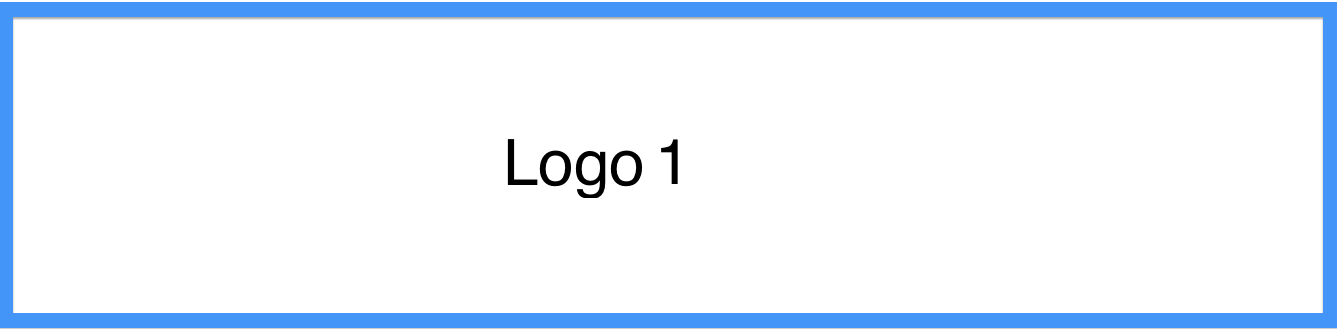
\includegraphics[width=0.4\textwidth,angle=45]{abb/logo1}
 \caption[Beispiel einer Bildbeschreibung]{Beispiel einer Bildbeschreibung\footnotemark}
\label{fig:beispiel1}
\end{figure}
\footnotetext{Bildquelle: Beispiel einer Bildquelle}

% Beispiel für Bildintegration
\begin{figure}[htb]
 \centering
 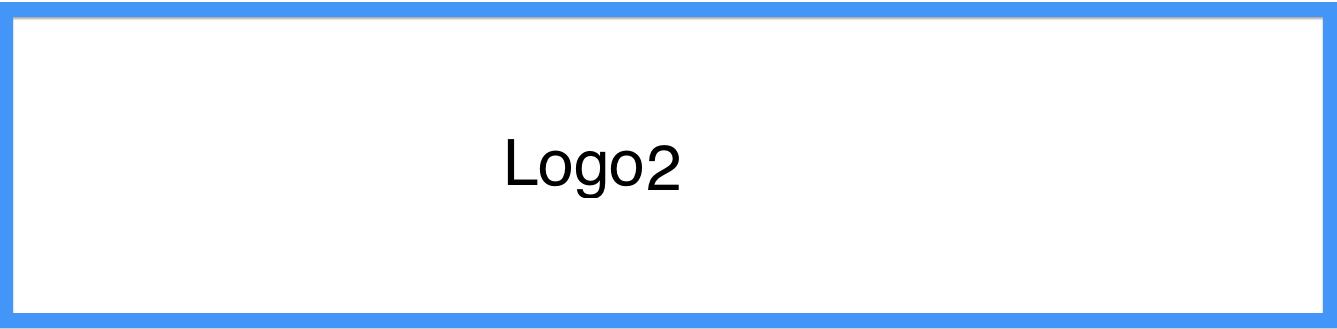
\includegraphics[width=0.3\textwidth,angle=0]{abb/logo2}
 \caption[Beschreibung]{Beschreibung}
\label{fig:Beschreibung}
\end{figure}

% Beispiel: Referenz auf Abbildung
Abbildung~\ref{fig:Beschreibung} [S.\pageref{fig:Beschreibung}]

% Beispiel: Tabelle 
\begin{center}
  \begin{tabular}{ | l | c | }
    \hline
    Überschrift 1 & Überschrift 2 \\ \hline \hline
    Info 1 & Info 2 \\ \hline
    Info 3 & Info 4 \\ \hline
    \hline
    \multicolumn{2}{|c|}{Info in einer Zelle} \\
    \hline
  \end{tabular}
\end{center}


% Beispiel für Quellcode Listings
\lstset{language=xml}
\begin{lstlisting}[frame=htrbl, caption={Die Datei {\normalfont \ttfamily  data-config.xml} dient als Beispiel für XML Quellcode}, label={lst:dataconfigxml}]
<dataConfig>
  <dataSource type="JdbcDataSource" 
              driver="com.mysql.jdbc.Driver"
              url="jdbc:mysql://localhost/bms_db"
              user="root" 
              password=""/>
  <document>
    <entity name="id"
        query="select id, htmlBody, sentDate, sentFrom, subject, textBody
        from mail">
    <field column="id" name="id"/>
    <field column="htmlBody" name="text"/>
    <field column="sentDate" name="sentDate"/>
    <field column="sentFrom" name="sentFrom"/>
    <field column="subject"  name="subject"/>
    <field column="textBody" name="text"/>
    </entity>
  </document>
</dataConfig>
\end{lstlisting}

\lstset{language=java}
\begin{lstlisting}[frame=htrbl, caption={Das Listing zeigt Java Quellcode}, label={lst:result2}]
/* generate TagCloud */
Cloud cloud = new Cloud();
cloud.setMaxWeight(_maxSizeOfText);
cloud.setMinWeight(_minSizeOfText);
cloud.setTagCase(Case.LOWER);
	    
/* evaluate context and find additional stopwords */
String query = getContextQuery(_context);
List<String> contextStoplist = new ArrayList<String>();
contextStoplist = getStopwordsFromDB(query);
	    
/* append context stoplist */
while(contextStoplist != null && !contextStoplist.isEmpty())
  _stoplist.add(contextStoplist.remove(0));
	    
/* add cloud filters */
if (_stoplist != null) {
  DictionaryFilter df = new DictionaryFilter(_stoplist);
  cloud.addInputFilter(df);
}
/* remove empty tags */
NonNullFilter<Tag> nnf = new NonNullFilter<Tag>();
cloud.addInputFilter(nnf);

/* set minimum tag length */
MinLengthFilter mlf = new MinLengthFilter(_minTagLength);
cloud.addInputFilter(mlf);

/* add taglist to tagcloud */
cloud.addText(_taglist);

/* set number of shown tags */	    
cloud.setMaxTagsToDisplay(_tagsToDisplay);
\end{lstlisting}


% Beispiel für Formeln
Die Zuordnung aller möglichen Werte, welche eine Zufallsvariable annehmen kann nennt man \emph{Verteilungsfunktion} von $X$.

\begin{quotation}
Die Funktion F: $\mathbb{R} \rightarrow$ [0,1] mit $F(t) = P (X \le t)$ heißt Verteilungsfunktion von $X$.\footnote{Mustermann, vgl.~\cite{mm2009}~[S.55]}
\end{quotation}

\begin{quotation}
Für eine stetige Zufallsvariable $X: \Omega \rightarrow \mathbb{R}$ heißt eine integrierbare, nichtnegative reelle Funktion $w: \mathbb{R} \rightarrow \mathbb{R}$ mit $F(x) = P(X \le x) = \int_{-\infty}^{x} w(t)dt$ die \emph{Dichte} oder \emph{Wahrscheinlichkeitsdichte} der Zufallsvariablen $X$.\footnote{Mustermann, vgl.~\cite{mf2005}~[S.56]}
\end{quotation}


% einfacher Zeilenabstand
\singlespacing
% Literaturliste soll im Inhaltsverzeichnis auftauchen
\newpage
\phantomsection
\addcontentsline{toc}{section}{Literaturverzeichnis}
% Literaturverzeichnis anzeigen
\renewcommand\refname{Literaturverzeichnis}
\bibliography{Hauptdatei}

%% Index soll Stichwortverzeichnis heissen
% \newpage
% % Stichwortverzeichnis soll im Inhaltsverzeichnis auftauchen
% \addcontentsline{toc}{section}{Stichwortverzeichnis}
% \renewcommand{\indexname}{Stichwortverzeichnis}
% % Stichwortverzeichnis endgültig anzeigen
% \printindex

\onehalfspacing
% evtl. Anhang
\newpage
\phantomsection
\addcontentsline{toc}{section}{Anhang}
\fancyhead[L]{Anhang} %Kopfzeile links
\subsection*{Anhang}\label{anhang}


\subsection *{Tabellen in der 3. Normalform}\label{3NF}


\begin{table}[H]
	\centering
	\begin{tabular}{|c|c|c|}
		\hline
		\underline{BenutzerNr} & Benutzername & Passwort \\
		\hline
		1 & Christine &  12345\\
		\hline
		2 & ADE &  asdfg\\
		\hline
		3 & Hugo &  yxcvb\\
		\hline
	\end{tabular}
	\caption{Die Tabelle Benutzerdaten in 3. Normalform.}
\end{table}

\begin{table}[H]
	\centering
	\begin{tabular}{|c|c|}
		\hline
		\underline{SelbstbedienungsstandNr} & Selbstbedienungsstandname \\
		\hline
		1 & Eierhütte \\
		\hline
		2 & Kartoffelhaus \\
		\hline
		3 & Stand1 \\
		\hline
	\end{tabular}
	\caption{Die Tabelle Selbstbedienungsstand in der 3. Normalform.}
\end{table}

\begin{table}[H]
	\centering
	\begin{tabular}{|c|c|c|}
		\hline
		\underline{SelbstbedienungsstandNr} & \underline{BenutzerNr} & RollenNr \\
		\hline
		1 & 1 &  1\\
		\hline
		2 & 1 &  2\\
		\hline
		3 & 2 &  1\\
		\hline
		3 & 3 &  1\\
		\hline
	\end{tabular}
	\caption{Die Tabelle Selbstbedienungsstand-Nutzer in der 3. Normalform.}
\end{table}

\begin{table}[H]
	\centering
	\begin{tabular}{|c|c|}
		\hline
		\underline{\underline{RollenNr}} & Benutzerrollename \\
		\hline
		1 & Admin  \\
		\hline
		2 & User \\
		\hline
	\end{tabular}
	\caption{Die Tabelle Benutzerrollen in der 3. Normalform.}
\end{table}


\begin{table}[H]
	\centering
	\begin{tabular}{|c|c|c|c|c|}
		\hline
		\underline{WarenNr} & Warenname & EinheitNr & Preis(€)& Bemerkung \\
		\hline
		1 & Ei & 1 &  0,20 & \\
		\hline
		2 & Kartoffeln & 2 & 5 & Sorte Annabelle \\
		\hline
	\end{tabular}
	\caption{Die Tabelle Waren in der 3. Normalform.}
\end{table}


\begin{table}[H]
	\centering
	\begin{tabular}{|c|c|}
		\hline
		\underline{Einheit-Nr}& Name der Einheit\\
		\hline
		1 & Stück\\
		\hline
		2 & KG \\
		\hline
	\end{tabular}
	\caption{Die Tabelle Einheit in der 3. Normalform.}
\end{table}

\begin{table}[H]
	\centering
	\begin{tabular}{|c|c|c|c|c|}
		\hline
		\underline{WareneingangsNr} & Datum & Wareneingang(Anzahl) & WarenNr & BenutzerNr \\
		\hline
		1 & 25.07.2021 & +100 & 2 & 1 \\
		\hline
		2 & 25.07.2021  & +80 & 1 & 1 \\
		\hline
		3 & 26.07.2021  & +60 & 2 & 1 \\
		\hline
		4 & 26.07.2021  &+5 & 2 &  2\\
		\hline
	\end{tabular}
	\caption{Die Tabelle Wareneingang in der 3. Normalform.}
\end{table}

\begin{table}[H]
	\centering
	\begin{tabular}{|c|c|c|c|c|c|}
		\hline
		\underline{Datum} & \underline{WarenNr} & BenutzerNr & Gezählt & Verkauft & Einnahmen(€) \\
		\hline
		25.07.2021 & 1 & 1 & 231 & 251 & 50,20 \\
		\hline
		26.07.2021 & 1 & 1 & 52 & 239 & 47,80 \\
		\hline
		26.07.2021 & 2 & 1 & 3 & 2 & 10 \\
		\hline
	\end{tabular}
	\caption{Die Tabelle Tagesabschluss in der 3. Normalform.} \label{3NF Tagesabschluss}
\end{table}

\newpage

%\subsection *{Entwurf der Schnittstellen}\label{Schnittstellen}

\textbf{Benutzer anlegen}

\textit{Client-Anfrage}
\\
Authentifizierung: JWT\\
Befehl: POST user/new\\
Daten: Benutzername, Passwort\\

\textit{Server-Antwort}
\\
Daten:\\
Erfolg: Statuscode 201\\
oder bei Misserfolg: Statuscode 400, Fehlermeldung: Dem Benutzer wurde bereits einen  Selbstbedienungsstand mit dem Namen XY zugewiesen.\\
oder bei einer ungültigen Authentifizierung: Statuscode 401 

\noindent\rule{\textwidth}{1pt}
\\
\textbf{Schnittstelle Tagesabschluss(EndOfTheDayController)}
\\
Der EndOfTheDayController stellt die folgenden Schnittstellen zur Verfügung:

\begin{itemize}
	\itemsep0pt
	\item  POST /endOfDay/
	\item  PUT /endOfDay/
	\item  GET /endOfDay/
\end{itemize}

Diese Schnittstellen dienen der Verwaltung des Tagesabschlusses, für jede Ware kann pro Tag nur ein Abschluss erstellt werden. Außerdem darf nur ein Benutzer mit Administratorrechten dieses ausführen.
Die Schnittstelle POST /endOfDay/ sorgt dafür das ein neuer Eintrag erstellt werden kann.
Mithilfe der Schnittstelle PUT /endOfDay/ kann dieser Eintrag editiert werden.
Die Schnittstelle GET /endOfDay/ übermittelt eine Auflistung, darin enthalten sind unter anderem die Angaben, der theoretisch verkauften Waren und theoretische Einnahmen (ohne Diebstahl, beschädigte Ware usw.). 
\\
\\
\textit{\underline{POST /endOfDay/}}
\\
\\
\NumTabs{4}				
Eingabeparameter: \tab				- LocalDate graduationDate (Datum des Tagesabschlusses)\\
\tab\tab								- String codesName (Name der Ware)		\\
\tab\tab								- String userName (Name des Benutzers)\\
\tab\tab								- String selfServiceStandName (Name des \\
\tab\tab 								Selbstbedienungsstandes)\\
\tab\tab								- int graduationCount (Die Anzahl der vorhanden Waren, \\
\tab \tab 								ermitteln durch zählen, wiegen o. Ä. )\\									
\\
Rückgabewerte: \tab 					Erfolg: HttpStatus.OK und Meldung.\\
\tab \tab 									Misserfolg: HttpStatus.NO CONTENT und Meldung\\
\\
Beispielrückgabelmeldung:	
\\
\\
\textit{\underline{PUT /endOfDay/}}
\\
\\
\NumTabs{4}				
Eingabeparameter: \tab				- Optional, LocalDate graduationDate (geändertes Datum \\
\tab\tab 							des Tagesabschlusses)\\
\tab\tab							- Optional,	String codesName (geänderter Name der Ware)		\\
\tab\tab							- Optional,	String userName (geänderter Name des Benutzers)\\
\tab\tab							- Optional,	int graduationCount (geänderte Anzahl der \\
\tab\tab vorhanden Waren)\\
\tab\tab											- LocalDate oldDate (Datum des alten Tagesabschlusses, \\
\tab\tab vor der Änderung)\\
\tab\tab												- String oldGoodsName (Name der alten Ware, \\
\tab\tab vor der Änderung)\\
\\
Rückgabewerte: \tab 					Erfolg: HttpStatus.OK und Meldung.\\
\tab \tab 									Misserfolg: HttpStatus.NO CONTENT und Meldung\\
\\
Beispielrückgabelmeldung:	
\\
\\
\\

%%%%%%%%%%%%%%%%%%%%%%%%%%%%%%%%%%%%%%%%%%%%%%%%%%%%%%%%%%%%%%%%%%%%%%%%%%%%%%%%%%%%%%%%%%%%%%%%%%%%%%%%%%%%%%%%%%%%%%%%%%%%%%%%%%%%%%%%%%%%%%%%%%%%%%%%%
\textbf{Schnittstelle Waren(GoodsController)}
\\
Der EndOfTheDayController stellt die folgenden Schnittstellen zur Verfügung:

\begin{itemize}
	\itemsep0pt
	\item  POST /goods/
	\item  PUT /goods/
	\item  DELETE /goods/
	\item  GET /goods/
	\item  GET /goods/{selfServiceStandName}/{userName}	
	\item  GET /goods//{selfServiceStandName}/{userName}/{goodsName}
\end{itemize}

Mithilfe dieser Schnittstellen lässt sich neue Ware anlegen (POST /goods/), verändern (PUT /goods/) oder auch löschen (DELETE /goods/). Diese Schnittstellen können nur von jemanden mit Administratorrechten genutzt werden. Eine Ware kann nur gelöscht werden, wenn diese nicht genutzt wird. Die beiden Schnittstellen GET /goods/ geben eine Übersicht der Waren zurück, dieses kann eine Liste oder eine einzelne Ware sein.
\\
\\
\textit{\underline{POST /endOfDay/}}
\\
\\
\NumTabs{4}				
Eingabeparameter: \tab			- String goodsName(Warenname)\\
\tab \tab                        		- String unitName	(Wareneinheit)\\
\tab \tab                         		- int goodsPrice (Preis der Ware)\\
\tab \tab                         		- String goodsNote (Bemerkung)    \\                  
\tab \tab                         		- String selfServiceStandName \\
\tab \tab								 (Name des Selbstbedienungsstandes)\\
\tab \tab                        		- String userName (Benutzername)\\
\\
Rückgabewerte: \tab 					Erfolg: HttpStatus.OK und Meldung.\\
\tab \tab 								Misserfolg: HttpStatus.NO CONTENT und Meldung\\
\\
Beispielrückgabelmeldung:	
\\
\\
\textit{\underline{PUT /endOfDay/}}
\\
\\
\NumTabs{4}				
Eingabeparameter: \tab			- String goodsName( Warenname)\\
\tab \tab                        		- optional String unitName	(geänderte Wareneinheit)\\
\tab \tab                         -	optional	int goodsPrice (geänderter Preis der Ware)\\
\tab \tab                         		- optional String goodsNote (geänderte Bemerkung)    \\                  
\tab \tab                         		- String selfServiceStandName \\
\tab \tab								(Name des Selbstbedienungsstandes)\\
\tab \tab                        		- String userName (Benutzername)\\
\tab \tab                        		- optional String changeGoodsName (Der neue Name, der Ware)\\
\\
Rückgabewerte: \tab 					Erfolg: HttpStatus.OK und Meldung.\\
\tab \tab 								Misserfolg: HttpStatus.NO CONTENT und Meldung\\
\\
Beispielrückgabelmeldung:	
\\
\\	
\textit{\underline{POST /endOfDay/}}
\\
\\
\NumTabs{4}				
Eingabeparameter: \tab			- String goodsName(Warenname)\\
\tab \tab                        		- String unitName	(Wareneinheit)\\
\tab \tab                         		- int goodsPrice (Preis der Ware)\\
\tab \tab                         		- String goodsNote (Bemerkung)    \\                  
\tab \tab                         		- String selfServiceStandName \\
\tab \tab								 (Name des Selbstbedienungsstandes)\\
\tab \tab                        		- String userName (Benutzername)\\
\\
Rückgabewerte: \tab 					Erfolg: HttpStatus.OK und Meldung.\\
\tab \tab 								Misserfolg: HttpStatus.NO CONTENT und Meldung\\
\\
Beispielrückgabelmeldung:	
\\
\\
\textit{\underline{DELETE /endOfDay/}}
\\
\\
\NumTabs{4}				
Eingabeparameter: \tab			- String goodsName( Warenname)\\                
\tab \tab                         		- String selfServiceStandName \\
\tab \tab								(Name des Selbstbedienungsstandes)\\
\tab \tab                        		- String userName (Benutzername)\\
\\
Rückgabewerte: \tab 					Erfolg: HttpStatus.OK und Meldung.\\
\tab \tab 								Misserfolg: HttpStatus.NO CONTENT und Meldung\\
\\
Beispielrückgabelmeldung:	
\\
\\
\textit{\underline{GET /goods//{selfServiceStandName}/{userName}}}
\\
\\
Rückgabewerte: \tab 					Erfolg: HttpStatus.OK und Meldung.\\
\\
Beispielrückgabelmeldung:	
\\
\\
\textit{\underline{GET /goods//{selfServiceStandName}/{userName}}}
\\
\\
Rückgabewerte: \tab 					Erfolg: HttpStatus.OK und Meldung.\\
\\
Beispielrückgabelmeldung:	
\\
\\
%%%%%%%%%%%%%%%%%%%%%%%%%%%%%%%%%%%%%%%%%%%%%%%%%%%%%%%%%%%%%%%%%%%%%%%%%%%%%%%%%%%%%%%%%%%%%%%%%%%%%%%%%%%%%%%%%%%%%%%%%%%%%%%%%%%%%%%%%%%%%%%%%%%%%%%%%

\textbf{Schnittstelle Warenname(GoodsNameController)}
\\
Der GoodsNameController stellt die folgenden Schnittstellen zur Verfügung:

\begin{itemize}
	\itemsep0pt
	\item  POST /goodsName/{goodsName}
	\item  PUT /goodsName/
	\item  DELETE /goodsName/
	\item  GET /goodsName/

\end{itemize}

Die Schnittstellen der Klasse GoodsNameController enthalten Schnittstellen die dafür verantwortlich sind Warennamen hinzuzufügen (POST /goodsName/), ändern (PUT /goodsName/) und löschen (DELETE /goodsName/). Außerdem kann eine Liste mit allen verfügbaren Namen ausgegeben werden.
Jeder Warenname kann nur einmalig vergeben werden. \\
Der Warennamen wie in einer separaten Tabelle gespeichert, dieses hat den Vorteil das Redundanzen vermieden werden. Außerdem geht so verhindert das ist unterschiedliche Schreibweisen für ein und dieselbe Ware existieren.
\\
\\
\textit{\underline{GET /goodsName/}}
\\
\\
\NumTabs{4}				
Eingabeparameter: \tab					- keine Variablen erforderlich
\\
Rückgabewerte: \tab 					Erfolg: Json Liste mit allen Warenamen.\\
\\
Beispielrückgabelmeldung:	
\\
\\
%§§§§§§§§§§§§§§§§§§§§§§§§§§§§§§§§§§§§§§§§§§§§§§§§§§
\\
\\
\textit{\underline{POST /goodsName/{goodsName}}}
\\
\\
Rückgabewerte: \tab 					Erfolg: HttpStatus Created\\
\tab \tab 								Misserfolg: HttpStatus No CONTENT\\
\\
Beispielrückgabelmeldung:	
\\
\\
%§§§§§§§§§§§§§§§§§§§§§§§§§§§§§§§§§§§§§§§§§§§§§§§§§§
\\
\\
\textit{\underline{DELETE /goodsName/{goodsName}}}
\\
\\
Rückgabewerte: \tab 					Erfolg: HttpStatus.OK\\
\tab \tab 								Misserfolg: HttpStatus Conflict\\
\\
Beispielrückgabelmeldung:	
\\
\\
%§§§§§§§§§§§§§§§§§§§§§§§§§§§§§§§§§§§§§§§§§§§§§§§§§§
\\
\\
\textit{\underline{DELETE /goodsName/{oldGoodsName}/{newGoodsName}}}
\\
\\
Rückgabewerte: \tab 					Erfolg: HttpStatus OK\\
\tab \tab 								Misserfolg: HttpStatus Conflict\\
\\
Beispielrückgabelmeldung:	
\\
\\
%§§§§§§§§§§§§§§§§§§§§§§§§§§§§§§§§§§§§§§§§§§§§§§§§§§
%%%%%%%%%%%%%%%%%%%%%%%%%%%%%%%%%%%%%%%%%%%%%%%%%%%%%%%%%%%%%%%%%%%%%%%%%%%%%%%%%%%%%%%%%%%%%%%%%%%%%%%%%%%%%%%%%%%%%%%%%%%%%%%%%%%%%%%%%%%%%%%%%%%%%%%%%
\textbf{Schnittstelle Wareneingang(EndOfTheDayController)}
\\
Der EndOfTheDayController stellt die folgenden Schnittstellen zur Verfügung:

\begin{itemize}
	\itemsep0pt
	\item  POST /receipt/
	\item  PUT /receipt/
	\item  DELETE /receipt/{receiptGoodsNr}
	\item  GET /receipt/{receiptGoodsNr}
	\item  GET /receipt/{selfServiceStandName}
	\item  GET /receipt/{selfServiceStandName}/{goodsName}
\end{itemize}

Mithilfe dieser Schnittstellen wird der Wareneingang und Warenausgang protokolliert. Mithilfe der Schnittstelle POST /receipt/ wird ein neuer Wareneingang oder Warenausgang hinzugefügt. PUT /receipt/ ändert diesen und DELETE /receipt/{receiptGoodsNr} löscht diesen Eintrag.
Die Schnittstelle GET /receipt/{receiptGoodsNr} übergibt einen einzelnen Datensatz. Eine Liste mit allen Eingängen und Ausgängen, einer bestimmten Ware überliefert die Schnittstelle GET /receipt/{selfServiceStandName}/{goodsName}. Die Schnittstelle GET /receipt/{selfServiceStandName} liefert ebenfalls eine Liste, allerdings mit allen Ein-und Ausgängen.  Bei den letzten beiden Schnittstellen muss der Selbstbedienungsstandnamen angeben werden, damit ein eindeutiger Zuordnung stattfinden kann. 
\\
\\
\textit{\underline{POST /receipt/}}
\\
\\
\NumTabs{4}				
Eingabeparameter: \tab			- LocalDate receiptDate(Datum Bestandsveränderung)\\
\tab \tab                        		- int goodsPieces\\
\tab \tab 								(Anzahl der Ware, die hinzugefügt oder entnommen wurde) \\
\tab \tab                         		- String goodsName \\
\tab \tab                         		- String userName \\                  
\tab \tab                         		- String selfServiceStandName\\
\\
Rückgabewerte: \tab 					Erfolg: HttpStatus OK und Meldung.\\
\tab \tab 								Misserfolg: HttpStatus NO CONTENT und Meldung\\
\\
Beispielrückgabelmeldung:	
\\
\\
%§§§§§§§§§§§§§§§§§§§§§§§§§§§§§§§§§§§§§§§§§§§§§§§§§§
\\
\\
\textit{\underline{PUT /receipt/}}
\\
\\
\NumTabs{4}				
Eingabeparameter: \tab			- int receiptID (ID)\\
\tab \tab                        		- optional LocalDate receiptDate(Datum Bestandsveränderung)\\\\
\tab \tab                        		- optional int goodsPieces\\
\tab \tab 								(Anzahl der Ware, die hinzugefügt oder entnommen wurde) \\
\tab \tab                         		- optional String goodsName \\
\tab \tab                         		- optional String userName \\                  
\\
Rückgabewerte: \tab 					Erfolg: HttpStatus OK \\
\tab \tab 								Misserfolg: HttpStatus NO CONTENT \\
\\
Beispielrückgabelmeldung:	
\\
\\
%§§§§§§§§§§§§§§§§§§§§§§§§§§§§§§§§§§§§§§§§§§§§§§§§§§
\\
\\
\textit{\underline{DELETE /receipt/{receiptGoodsNr}}}
\\              
\\
Rückgabewerte: \tab 					Erfolg: HttpStatus OK \\
\tab \tab 								Misserfolg: HttpStatus Conflict \\
\\
Beispielrückgabelmeldung:	
\\
\\
%§§§§§§§§§§§§§§§§§§§§§§§§§§§§§§§§§§§§§§§§§§§§§§§§§§
\\
\\
\textit{\underline{GET /receipt/{receiptGoodsNr}}}
\\              
\\
Rückgabewerte: \tab 					Erfolg: ein Datensatz \\
\\
Beispielrückgabelmeldung:	
\\
\\
%§§§§§§§§§§§§§§§§§§§§§§§§§§§§§§§§§§§§§§§§§§§§§§§§§§
\\
\\
\textit{\underline{GET /receipt/{selfServiceStandName}}}
\\                
\\
Rückgabewerte: \tab 					Erfolg: Liste mit allen Datensätzen, die dem Selbstbedingungsstand zugeordnet sind\\
\\
Beispielrückgabelmeldung:	
\\
\\
%§§§§§§§§§§§§§§§§§§§§§§§§§§§§§§§§§§§§§§§§§§§§§§§§§§
\\
\\
\textit{\underline{GET /receipt/{selfServiceStandName}}}
\\                
\\
Rückgabewerte: \tab 					Erfolg: Liste mit allen Datensätzen, die dem Selbstbedingungsstand zugeordnet sind und die dem Warennamen entsprechen\\
\\
Beispielrückgabelmeldung:	
\\
\\
%%%%%%%%%%%%%%%%%%%%%%%%%%%%%%%%%%%%%%%%%%%%%%%%%%%%%%%%%%%%%%%%%%%%%%%%%%%%%%%%%%%%%%%%%%%%%%%%%%%%%%%%%%%%%%%%%%%%%%%%%%%%%%%%%%%%%%%%%%%%%%%%%%%%%%%%%
\textbf{Schnittstelle Benutzerrollen(RoleController)}
\\
Der RoleController stellt die folgenden Schnittstellen zur Verfügung:

\begin{itemize}
	\itemsep0pt
	\item  GET /role/
	\item PUT /role//userRole/
\end{itemize}

Diese Schnittstelle GET /role/ gibt eine sortierte Liste mit allen verfügbaren Benutzerrollen zurück.
PUT /role//userRole/ bewirkt das eine Benuterrolle eines Benutzer geändert wird. Nur ein Benutzer mit Administratorrechten darf Benutzerrollen ändern.
\\
\\
\textit{\underline{GET /role/}}
\\
\\
Rückgabewerte: \tab 					Erfolg: HttpStatus OK und Liste mit allen Benutzerrollen.\\
\\
Beispielrückgabelmeldung:	
\\
\\
%§§§§§§§§§§§§§§§§§§§§§§§§§§§§§§§§§§§§§§§§§§§§§§§§§§
\\
\\
\textit{\underline{PUT /role//userRole/}}
\\
\\
\NumTabs{4}				
Eingabeparameter: \tab			- String changeUserName (Benutzer dessen Rolle geändert wird)\\
\tab \tab                        		- String userName (Name des Benutzer, der die Benutzerrolle ändert)\\\\
\tab \tab                        		- String selfServiceStandName\\
\tab \tab                         		- optional String goodsName \\
\tab \tab                         		- String newRole (Name der neuen Role) \\                  
\\
Rückgabewerte: \tab 					Erfolg: HttpStatus OK \\
\tab \tab 								Misserfolg: HttpStatus NO CONTENT \\
\\
Beispielrückgabelmeldung:	
\\
\\
%%%%%%%%%%%%%%%%%%%%%%%%%%%%%%%%%%%%%%%%%%%%%%%%%%%%%%%%%%%%%%%%%%%%%%%%%%%%%%%%%%%%%%%%%%%%%%%
\textbf{Schnittstelle Selbstbedingungsstand (SelfServiceStandController)}
\\
Der SelfServiceStandController stellt die folgenden Schnittstellen zur Verfügung:

\begin{itemize}
	\itemsep0pt
	\item  POST /selfServiceStand/{userName}/{selfServiceStandName}
	\item  POST /selfServiceStand/addUser/
	\item  DELETE /selfServiceStand/{removeUserName}/{userName}/{selfServiceStandName}
	\item GET /selfServiceStand/{selfServiceStandName}
\end{itemize}


Diese Schnittstellen helfen bei der Verwaltung eines Selbstbedienungsstandes. Ein neuer Selbstbedienungsstand wird mit der Schnittstelle POST /selfServiceStand/{userName}/{selfServiceStandName} erstellt, der Benutzer der diesen erstellt hat, erhält Administratorrechte.\\ Die Schnittstelle POST /selfServiceStand/addUser/ fügt einen bereits existierenden Benutzer, einen Selbstbedienungsstand hinzu, dabei kann die Benutzerrolle frei gewählt werden. Sobald ein Benutzer entfernt werden soll, hilft die Schnittstelle DELETE /selfServiceStand/{removeUserName}/{userName}/{selfServiceStandName}.
Eine Liste mit allen Benutzern die dem Selbstbedienungsstand zugeordnet sind, wird mithilfe der Schnittstelle GET /selfServiceStand/{selfServiceStandName} ausgeben.
\\
\\
\textit{\underline{POST /selfServiceStand/{userName}/{selfServiceStandName}}}
\\
\\
Rückgabewerte: \tab 					Erfolg: HttpStatus OK und Meldung.\\
\tab \tab 								Misserfolg: HttpStatus Conflict und Meldung\\
\\
Beispielrückgabelmeldung:	
\\
\\
%§§§§§§§§§§§§§§§§§§§§§§§§§§§§§§§§§§§§§§§§§§§§§§§§§§
\\
\\
\textit{\underline{POST /selfServiceStand/addUser/}}
\\
\\
\NumTabs{4}				
Eingabeparameter: \tab			- String addingUserName (Benutzer der hinzugefügt wird)\\
\tab \tab                        		- String userName (Name des Benutzer, der den neuen Benutzer hinzufügt)\\\\
\tab \tab                        		- String selfServiceStandName\\                 
\\
Rückgabewerte: \tab 					Erfolg: HttpStatus OK \\
\tab \tab 								Misserfolg: HttpStatus Conflict \\
\\
Beispielrückgabelmeldung:	
\\
\\
%%%%%%%%%%%%%%%%%%%%%%%%%%%%%%%%%%%%%%%%%%%%%%%%%%%%%%%%%%%%%%%%%%%%%%%%%%%%%%%%%%%%%%%%%%%%%%%
\textit{\underline{DELETE /selfServiceStand/{removeUserName}/{userName}/{selfServiceStandName}}}
\\
\\
Rückgabewerte: \tab 					Erfolg: HttpStatus OK und Meldung.\\
\tab \tab 								Misserfolg: HttpStatus Conflict und Meldung\\
\\
Beispielrückgabelmeldung:	
\\
\\
%§§§§§§§§§§§§§§§§§§§§§§§§§§§§§§§§§§§§§§§§§§§§§§§§§§
%%%%%%%%%%%%%%%%%%%%%%%%%%%%%%%%%%%%%%%%%%%%%%%%%%%%%%%%%%%%%%%%%%%%%%%%%%%%%%%%%%%%%%%%%%%%%%%%%%%%%%%%%%%%%%%%%%%%%%%%%%%%%%%%%%%%%%%%%%%%%%%%%%%%%%%%%
\textbf{Schnittstelle Einheiten(UnitController)}
\\
Der UnitController stellt die folgenden Schnittstellen zur Verfügung:

\begin{itemize}
	\itemsep0pt
	\item  POST /unit/{unitName}
	\item  PUT /unit/{oldUnitName}/{newUnitName}
	\item  DELETE /unit//{unitName}
	\item  GET /unit//{unitName}
\end{itemize}
Einheiten wie z.B. Stück, KG, Sack usw. können mit der Schnittstelle POST /unit/ erstellt werden. Verändert werden können diese mit der Schnittstelle PUT /unit/. Soll eine Einheit gelöscht werden ist dieses mit der Schnittstelle DELETE /unit//{unitName} möglich. Allerdings können Änderung und Löschungen nur durchgeführt werden, wenn die Einheit noch nicht verwendet wird.
Eine Liste der verfügbaren Einheiten gibt die Schnittstelle GET /unit//{unitName} aus.
\\
\\
\textit{\underline{POST /unit/{unitName}}}
\\
\\
Rückgabewerte: \tab 					Erfolg: HttpStatus Create und Meldung.\\
\tab \tab 								Misserfolg: HttpStatus No Content\\
\\
Beispielrückgabelmeldung:	
\\
\\
%§§§§§§§§§§§§§§§§§§§§§§§§§§§§§§§§§§§§§§§§§§§§§§§§§§
\textit{\underline{PUT /unit/{oldUnitName}/{newUnitName}}}
\\
\\
Rückgabewerte: \tab 					Erfolg: HttpStatus OK und Meldung.\\
\tab \tab 								Misserfolg: HttpStatus Conflict\\
\\
Beispielrückgabelmeldung:	
\\
\\
%§§§§§§§§§§§§§§§§§§§§§§§§§§§§§§§§§§§§§§§§§§§§§§§§§§
\textit{\underline{DELETE /unit//{unitName}}}
\\
\\
Rückgabewerte: \tab 					Erfolg: HttpStatus OK und Meldung.\\
\tab \tab 								Misserfolg: HttpStatus Conflict\\
\\
Beispielrückgabelmeldung:	
\\
\\
%§§§§§§§§§§§§§§§§§§§§§§§§§§§§§§§§§§§§§§§§§§§§§§§§§§
\textit{\underline{GET /unit//{unitName}}}
\\
\\
Rückgabewerte: \tab 					Erfolg: HttpStatus OK und Liste mit allen Einheiten.\\
\\
Beispielrückgabelmeldung:	
\\
\\
%§§§§§§§§§§§§§§§§§§§§§§§§§§§§§§§§§§§§§§§§§§§§§§§§§§
%%%%%%%%%%%%%%%%%%%%%%%%%%%%%%%%%%%%%%%%%%%%%%%%%%%%%%%%%%%%%%%%%%%%%%%%%%%%%%%%%%%%%%%%%%%%%%%%%%%%%%%%%%%%%%%%%%%%%%%%%%%%%%%%%%%%%%%%%%%%%%%%%%%%%%%%%
\textbf{Schnittstelle Wareneingang(EndOfTheDayController)}
\\
Der EndOfTheDayController stellt die folgenden Schnittstellen zur Verfügung:

\begin{itemize}
	\itemsep0pt
	\item  POST /user/newAdmin
	\item  POST /user/newUser
	\item  PUT /user/
	\item  GET /user/{username}
\end{itemize}

Die Benutzerverwaltung kann mithilfe nachfolgender Schnittstellen durchgeführt werden. Ein neuer Benutzer und ein neuer Selbstbedienungsstand werden mit der Schnittstelle POST /user/newAdmin erstellt. Der neu erstellte Benutzer, wird automatisch dem erstellten Selbstbedienungsstand als Administrator zugeordnet. Der Name des Selbstbedienungsstandes und des Benutzers dürfen noch nicht vergeben sein.
\\
Ein Administrator eines  Selbstbedienungsstandes kann einen neuen Benutzer zu diesem hinzufügen, der Benutzer wird dabei neu erstellt, die Benutzerrolle kann frei gewählt werden, dieses geschieht mit der Schnittstelle POST /user/newUser. 
\\
Sobald ein neuer Benutzer erstellt wird wie zuerst überprüft ob der Benutzername bereits vergeben ist, sollte dieses der Fall sein, kann der Benutzer nicht erstellt werden. Die Schnittstelle PUT /user/ ist zum Editieren des Benutzers gedacht. Ein einzelner Benutzer kann mit der Schnittstelle GET /user/{username} ausgegeben werden.
\\
\\
\textit{\underline{POST /user/newAdmin}}
\\
\\
\NumTabs{4}				
Eingabeparameter: \tab			- String userName (Benutzername)\\
\tab \tab                        		- String userPassword (Passwort)\\
\tab \tab                         		- String selfServiceStandName (Name des Selbstbedienungsstandes, der neu erstellt wird) \\
\tab \tab                         		- String email (E-Mail Adresse)\\                  
\\
Rückgabewerte: \tab 					Erfolg: HttpStatus Createt und Meldung.\\
\tab \tab 								Misserfolg: HttpStatus NO CONTENT und Meldung\\
\\
Beispielrückgabelmeldung:	
\\
\\
%§§§§§§§§§§§§§§§§§§§§§§§§§§§§§§§§§§§§§§§§§§§§§§§§§§
\textit{\underline{POST /user/newUser}}
\\
\\
\NumTabs{4}				
Eingabeparameter: \tab			- String userName (Benutzername)\\
\tab \tab                        		- String userPassword (Passwort)\\
\tab \tab                         		- String selfServiceStandName (Name des Selbstbedienungsstandes, zu dem der Benutzer hinzugefügt wird. ) \\
\tab \tab                         		- String email (E-Mail Adresse) \\                  
\\
Rückgabewerte: \tab 					Erfolg: HttpStatus Createt und Meldung.\\
\tab \tab 								Misserfolg: HttpStatus NO CONTENT und Meldung\\
\\
Beispielrückgabelmeldung:	
\\
\\
%§§§§§§§§§§§§§§§§§§§§§§§§§§§§§§§§§§§§§§§§§§§§§§§§§§
\textit{\underline{PUT /user/}}
\\
\\
\NumTabs{4}				
Eingabeparameter: \tab			- optional String userName (Benutzername)\\
\tab \tab                        		- optional String userPassword (Passwort)\\
\tab \tab                         		- optional String selfServiceStandName (Name des Selbstbedienungsstandes, zu dem der Benutzer hinzugefügt wird. ) \\
\tab \tab                         		- optional String email (E-Mail Adresse)\\
\tab \tab                         		- optional String changeUserName (neuer Benutzername)\\                   
\\
Rückgabewerte: \tab 					Erfolg: HttpStatus Ok und Meldung.\\
\tab \tab 								Misserfolg: HttpStatus NO Conflict und Meldung\\
\\
Beispielrückgabelmeldung:	
\\
\\
%§§§§§§§§§§§§§§§§§§§§§§§§§§§§§§§§§§§§§§§§§§§§§§§§§§
\textit{\underline{GET /user/{username}}}
\\                  
\\
Rückgabewerte: \tab 					Erfolg: HttpStatus Createt und Benutzerdetails\\
\\
Beispielrückgabelmeldung:	
\\
\\
%§§§§§§§§§§§§§§§§§§§§§§§§§§§§§§§§§§§§§§§§§§§§§§§§§§
%\newpage

\subsection *{Quellcode Server (Ausschnitt)}\label{QuellcodeServer}


\lstset{language=java}
\begin{lstlisting}[frame=tb, caption={Das Listing zeigt die Klasse EndOfTheDay im Paket model}, label={lst:EndOfTheDay}]
import lombok.Getter;
import lombok.Setter;

import javax.persistence.*;

/**
* Class represents the table "tb_end of_the_day".
*/
@Table(name = "tb_end of_the_day", indexes = {
	@Index(name = "cl_user_nr", columnList = "cl_user_nr"),
	@Index(name = "cl_goods_nr", columnList = "cl_goods_nr"),
	@Index(name = "cl_self_service_stand_nr", 
	columnList = "cl_self_service_stand_nr")
})
@Setter
@Getter
@Entity
public class EndOfTheDay {
	
	/**
	* ID End of the Day.
	*/
	@EmbeddedId
	private EndOfTheDayId id;
	
	/**
	* Refers to a user ID.
	*/
	@ManyToOne
	@JoinColumn(name = "cl_user_nr")
	private User userNr;
	
	/**
	* Refers to a self-Service-Stand name.
	*/
	@ManyToOne
	@JoinColumn(name = "cl_self_service_stand_nr")
	private SelfServiceStand selfServiceStandName;
	
	/**
	* The number of goods counted.
	*/
	@Column(name = "cl_graduation_count")
	private Integer graduationCount;
	
	/**
	* The number of computationally determined goods sold.
	*/
	@Column(name = "cl_graduation_sold")
	private Integer graduationSold;
	
	/**
	* The number of mathematically determined income in euros.
	*/
	@Column(name = "cl_graduation_revenue")
	private Double graduationRevenue;
}
\end{lstlisting}

%##############################################################################################

\lstset{language=java}
\begin{lstlisting}[frame=tb, caption={Das Listing zeigt die Klasse EndOfTheDayId im Paket model}, label={lst:EndOfTheDayId}]
/**
* Class represents the table ID "tb_end of_the_day".
*/
@Getter
@Setter
@Embeddable
public class EndOfTheDayId implements Serializable {
	
	/**
	* serialVersionUID
	*/
	private static final long serialVersionUID = 4548732131340178144L;
	
	/**
	* End of the day date.
	*/
	@Column(name = "cl_graduation_date", nullable = false)
	private LocalDate graduationDate;
	
	/**
	* The commodity number.
	*/
	@Column(name = "cl_goods_nr", nullable = false)
	private Integer goodsNr;
	
	/**
	* Overwritten hash code method.
	*
	* @return Objects
	*/
	@Override
	public int hashCode() {
		return Objects.hash(goodsNr, graduationDate);
	}
	
	/**
	* Overwritten equals method.
	*
	* @param o goodsNr and graduationDate
	* @return Objects
	*/
	@Override
	public boolean equals(Object o) {
		if (this == o) return true;
		if (o == null || Hibernate.getClass(this) != Hibernate.getClass(o)) return false;
		EndOfTheDayId entity = (EndOfTheDayId) o;
		return Objects.equals(this.goodsNr, entity.goodsNr) &&
		Objects.equals(this.graduationDate, entity.graduationDate);
	}
}
\end{lstlisting}

%##############################################################################################

\lstset{language=java}
\begin{lstlisting}[frame=tb, caption={Das Listing zeigt das Interface ReceiptGoodRepository im Paket repository}, label={lst:ReceiptGoodRepository}]
/**
* This class contains the database queries of the table tb_receipt_goods.
*/
@Repository
public interface ReceiptGoodRepository extends JpaRepository<ReceiptGoods, Integer> {
	
	/**
	* Query, finds a record with the incoming ID.
	* @param receiptGoodId The receipt goods Id.
	* @return record receiptGoods
	*/
	ReceiptGoods findByReceiptGoodId(Integer receiptGoodId);
	
	/**
	* Query, provides a list of all self-service booths that have the ID entered.
	* @param selfServiceStandNId The self-service-stand Id.
	* @return list receiptGoods
	*/
	List<ReceiptGoods> findBySelfServiceStandNr_SelfServiceStandNIdOrderByDateReceiptAsc(Integer selfServiceStandNId);
	
	/**
	* Query, provides a list of all self-service booths that have the ID and product name entered.
	* @param goodsName The goods name.
	* @param selfServiceStandNId The self-service-stand Id.
	* @return list receiptGoods
	*/
	List<ReceiptGoods> findByGoodsNr_GoodsNameNr_GoodsNameAndSelfServiceStandNr_SelfServiceStandNId(String goodsName, Integer selfServiceStandNId);
	
	/**
	* Query, finds a list of all dates and goods In that match.
	* @param dateReceipt The receipt date.
	* @param goodsId The goods ID.
	* @return list receiptGoods
	*/
	List<ReceiptGoods> findByDateReceiptAndGoodsNr_GoodsId(LocalDate dateReceipt, Integer goodsId);
}
\end{lstlisting}
%##############################################################################################

\lstset{language=java}
\begin{lstlisting}[frame=tb, caption={Das Listing zeigt die Klasse UnitController im Paket controller}, label={lst:UnitController}]
/**
* The role Controller class outputs a list of all existing units.
* It is possible to create new units.
* Units can also be changed and deleted, but only if they are not yet used in another table.
*
* <p>
* Provides the following endpoints: <br>
* - GET /role/ <br>
* - POST /role/{unitName} <br>
* - DELETE /role/{oldUnitName} <br>
* - PUT /role/{oldUnitName}/{newUnitName} <br>
*/
@RestController
@RequestMapping("/unit")
public class UnitController {
	
	/**
	* Logger of the unitController class.
	*/
	private static final Logger LOGGER = LoggerFactory.getLogger(UnitController.class);
	
	/**
	* unitRepository to handle unit information.
	*/
	private final UnitRepository unitRepository;
	
	/**
	* goodsRepository to handle goods information.
	*/
	private final GoodsRepository goodsRepository;
	
	public UnitController(UnitRepository unitRepository, GoodsRepository goodsRepository) {
		this.unitRepository = unitRepository;
		this.goodsRepository = goodsRepository;
	}
	
	/**
	* Method returns a sorted list with all units.
	*
	* @return json list with all units
	*/
	@GetMapping(path = "/", produces = MediaType.APPLICATION_JSON_VALUE)
	private ResponseEntity<Object> getUnits() {
		
		//Query sorted list, sorted by unit name
		return new ResponseEntity<>(unitRepository.findByOrderByUnitNameAsc(), HttpStatus.OK);
	}
	
	/**
	* Method creates a new unit, but only if it does not yet exist.
	*
	* @param unitName Name of the unit
	* @return Http Status code: Create if a new unit has been created, otherwise no content
	* and created unit.
	*/
	@PostMapping(path = "/{unitName}", produces = MediaType.APPLICATION_JSON_VALUE)
	private ResponseEntity<Unit> createUnit(@PathVariable String unitName) {
		
		//excess whitespace is removed
		unitName = unitName.trim();
		
		Unit newUnit = null;
		
		//It is checked whether the unit already exists.
		if (!unitRepository.existsByUnitNameIs(unitName)) {
			
			//save the new unit
			newUnit = unitRepository.save(new Unit(unitName));
			
			LOGGER.info("The unit " + unitName + " has been created.");
		} else {
			LOGGER.info("The unit " + unitName + " is already there.");
		}
		
		// Set the http status by unit; CREATED if it is null, NO_CONTENT otherwise
		final HttpStatus httpStatus = null != newUnit
		? HttpStatus.CREATED
		: HttpStatus.NO_CONTENT;
		
		return new ResponseEntity<>(newUnit, httpStatus);
	}
	
	/**
	* The method only deletes a unit from the list if it has not yet been used.
	*
	* @param unitName unit name
	* @return message in Json format and Http status code
	*/
	@DeleteMapping(path = "/{unitName}", produces = MediaType.APPLICATION_JSON_VALUE)
	private ResponseEntity<JSONObject> deleteUnit(@PathVariable String unitName) {
		
		//create new json object
		JSONObject message = new JSONObject();
		
		//excess whitespace is removed
		unitName = unitName.trim();
		
		//It is checked whether the unit is not used in the "goods" table.
		if (!goodsRepository.existsByGoodsUnitNr_UnitName(unitName)) {
			
			Unit deleteUnit = new Unit();
			deleteUnit.setUnitId(unitRepository.findByUnitName(unitName).getUnitId());
			
			//Delete Unit at the database
			unitRepository.delete(deleteUnit);
			
			LOGGER.info("The unit " + unitName + " has been deleted.");
			message.put("Message", "The unit " + unitName + " has been deleted.");
			return new ResponseEntity<>(message, HttpStatus.OK);
		} else {
			LOGGER.info("The unit " + unitName + " is already in use. Deletion is no longer possible.");
			message.put("Message", "The unit " + unitName + " is already in use. Deletion is no longer possible.");
			return new ResponseEntity<>(message, HttpStatus.CONFLICT);
		}
	}
	
	/**
	* The method only changes the name of a unit if it has not yet been used in the Goods table.
	*
	* @param oldUnitName old unit name
	* @param newUnitName new unit name
	* @return message in Json format and Http status code
	*/
	@PutMapping(path = "/{oldUnitName}/{newUnitName}", produces = MediaType.APPLICATION_JSON_VALUE)
	private ResponseEntity<JSONObject> updateUnit(@PathVariable String oldUnitName, @PathVariable String newUnitName) {
		
		//create new json object
		JSONObject message = new JSONObject();
		
		//excess whitespace is removed
		oldUnitName = oldUnitName.trim();
		newUnitName = newUnitName.trim();
		
		//It is checked whether the unit is not used in the "goods" table.
		if (!goodsRepository.existsByGoodsUnitNr_UnitName(oldUnitName)) {
			
			Unit changeUnit = new Unit();
			changeUnit.setUnitId(unitRepository.findByUnitName(oldUnitName).getUnitId());
			
			changeUnit.setUnitName(newUnitName);
			
			//change unit at the database
			unitRepository.save(changeUnit);
			
			LOGGER.info("The name of the unit has been changed from " + oldUnitName + " to " + newUnitName + ".");
			message.put("Message", "The name of the unit has been changed from " + oldUnitName + " to " + newUnitName + ".");
			return new ResponseEntity<>(message, HttpStatus.OK);
		} else {
			LOGGER.info("The unit " + oldUnitName + " is already in use. Change is no longer possible.");
			message.put("Message", "The unit " + oldUnitName + " is already in use. Change is no longer possible.");
			return new ResponseEntity<>(message, HttpStatus.CONFLICT);
		}
	}
}
\end{lstlisting}













\subsection *{Quellcode Client (Ausschnitt)}\label{QuellcodeClient}

\lstset{language=java}
\begin{lstlisting}[frame=tb, caption={Das Listing zeigt die CSS-Datei main-screen.component }, label={lst:main-screen.component}]
.container {
	display: grid;
	grid-template-columns: 0.5fr 2fr 8fr 2fr 0.5fr;
	grid-template-rows: 0.4fr 3.4fr 0.4fr 0.4fr;
	gap: 0px 0px;
	grid-auto-flow: row;
	grid-template-areas:
	"navbar navbar navbar navbar navbar"
	"main main main main main"
	"selectSelf selectSelf . . ."
	"footer footer footer footer footer";
}

.navbar {
	grid-area: navbar;
	background: var(--colorGray);
}

.main {
	grid-area: main;
	background: white;
}

.footer {
	grid-area: footer;
	background: var(--colorGray);
}

.selectSelf {
	grid-area: selectSelf;
	background: white;
}

html,
body {
	height: 100%;
	background: radial-gradient(var(--colorBackground2), var(--colorBackground1));
	overflow: hidden;
}

.container-main-screen {
	background: white;
}	
\end{lstlisting}
%##############################################################################################
\lstset{language=java}
\begin{lstlisting}[frame=tb, caption={Das Listing zeigt die CSS-Datei main-screen.component }, label={lst:main-screen.component}]
const myRoutes: Routes = [
{
	path: '',
	component: MainScreenComponent,
	children: [
	{
		path: 'goods',
		component: GoodsComponent,
		children: [
		{
			path: 'overview',
			component: OverviewGoodsComponent
		},
		{
			path: 'new',
			component: NewGoodsComponent
		},
		{
			path: 'change',
			component: ChangeGoodsComponent
		}, {
			path: 'settings',
			component: SettingsGoodsComponent
		}
		]
	},
	{
		path: 'receipt',
		component: ReceiptComponent,
		children: [
		{
			path: 'new',
			component: NewReceiptComponent
		},
		{
			path: 'overview',
			component: OverviewReceiptComponent
		},
		]
	},
	{
		path: 'user',
		component: UserComponent,
		children: [
		{
			path: 'change',
			component: ChangeUserComponent
		},
		{
			path: 'create',
			component: CreateUserComponent
		},
		{
			path: 'overview',
			component: OverviewUserComponent
		}
		]
	},
	{
		path: 'statistics',
		component: StatisticsComponent,
		children: [
		{
			path: 'month',
			component: MonthComponent
		},
		{
			path: 'year',
			component: YearComponent
		}
		]
	},
	{
		path: 'self',
		component: SelfServiceStandComponent,
		children: [
		{
			path: 'add',
			component: AddUserSelfComponent
		},
		{
			path: 'change',
			component: ChangeSelfComponent
		},
		{
			path: 'overview',
			component: OverviewSelfComponent
		}
		]
	},
	{
		path: 'end',
		component: EndOfDayComponent,
		children: [
		{
			path: 'overview',
			component: OverviewEndComponent
		},
		{
			path: 'new',
			component: NewEndComponent
		},
		{
			path: 'create',
			component: EndOfDayPdfComponent
		}
		]
	},
	{
		path: '',
		component: MainMenuComponent
	},
	{
		path:'**',
		component: PageNotFoundComponent,
	},
	]
}
]

@NgModule({
	declarations: [],
	imports: [
	CommonModule,
	RouterModule.forChild((myRoutes))
	],
	exports: [RouterModule]
})
export class MainScreenRoutesModule {
}
\end{lstlisting}
%##############################################################################################

\lstset{language=java}
\begin{lstlisting}[frame=tb, caption={Das Listing zeigt die TypeScript-Datei change-goods.ts }, label={lst:main-screen.component2}]

/**
* Class provides an overview of all goods.
*/
export class OverviewGoodsComponent implements OnInit {
	
	//empty list goods
	goodsList: Goods[] = [];
	
	//Heading of the table
	header: string[] = ['Warenname', 'Einheit', 'Preis', 'Bemerkung', 'im Verkauf'];
	
	//Saves whether a result was found
	searchResult: boolean = true;
	
	//List of search results
	searchResultList: Goods[] = [];
	
	
	constructor(private client: HttpClient,
	private communication: ServerCommunicationServiceService
	) {
	}
	
	ngOnInit(): void {
		this.loadGoods();
		this.searchResultList = this.goodsList;
	}
	
	//Filter the list of goods according to the search results and save them in the list
	search(event: Event) {
		
		//Old search results are deleted
		this.searchResultList = [];
		
		//Saves the keystrokes
		const filterValue = (event.target as HTMLInputElement).value;
		
		//Searches the list for the word
		for (let key in this.goodsList) {
			if (this.goodsList.hasOwnProperty(key)) {
				if (
				this.goodsList[key].goodsName.includes(filterValue) ||
				this.goodsList[key].unitName.includes(filterValue) ||
				this.goodsList[key].goodsPrice.toString().includes(filterValue) ||
				this.goodsList[key].goodsNote.includes(filterValue)
				) {
					//Saves all found experiences in the list
					this.searchResultList.push((this.goodsList[key]));
				}
			}
			//If not found, the variable is set to false.
			this.searchResult = this.searchResultList.length > 0;
		}
	}
	
	// Loads a list of goods from the server
	private loadGoods() {
		
		//set url
		let url = 'goods/' + localStorage.getItem('key_selfServiceStand_name');
		
		//communication Server
		this.communication
		.serverCommunication(url, '', 'get', true)
		.subscribe((response: any) => {
			
			//Saves the goods in a list
			for (var entry of response) {
				this.goodsList.push({
					goodsId: entry.goodsId,
					goodsName: entry.goodsNameNr.goodsName,
					unitName: entry.goodsUnitNr.unitName,
					goodsPrice: entry.goodsPrice,
					goodsNote: entry.goodsNote,
					goodsActive: entry.goodsActive
				});
			}
		}, error => {
			console.log(error);
		}
		);
	}
}
\end{lstlisting}
%##############################################################################################
\newpage









% Eidesstattliche Erklärung
\newpage
\phantomsection
\addcontentsline{toc}{section}{Eidesstattliche Erklärung}
\section*{Eidesstattliche Erklärung}
\thispagestyle{empty}

\begin{verbatim}

\end{verbatim}

\begin{LARGE}Eidesstattliche Erklärung zur Projektarbeit\end{LARGE}
\begin{verbatim}


\end{verbatim}
Ich versichere, die von mir vorgelegte Arbeit selbstständig verfasst zu haben. Alle Stellen, die wörtlich oder sinngemäß aus veröffentlichten oder nicht veröffentlichten Arbeiten anderer entnommen sind, habe ich als entnommen kenntlich gemacht. Sämtliche Quellen und Hilfsmittel, die ich für die Arbeit benutzt habe, sind angegeben. Die Arbeit hat mit gleichem Inhalt bzw. in wesentlichen Teilen noch keiner anderen Prüfungsbehörde vorgelegen.



\begin{displaymath}
% use packages: array
\begin{array}{ll}
Unterschrift:~~~~~~~~~~~~~~~~~~~~~~~~~~~~~~~~~~~~~~~~~~
& Ort, Datum:~~~~~~~~~~~~~~~~~~~~~~~~~~~~~~~~~~~~~~~~~~
\end{array}
\end{displaymath}

\begin{figure}[h]
	\begin{minipage}[b]{.4\linewidth} % [b] => Ausrichtung an \caption
	
\includegraphics[width=0.7\linewidth]{abb/unterschrift}
	\end{minipage}
	\hspace{.1\linewidth}% Abstand zwischen Bilder
	\begin{minipage}[b]{.4\linewidth} % [b] => Ausrichtung an \caption
	
\includegraphics[width=0.6\linewidth]{abb/ort}
	\end{minipage}
\end{figure}






% leere Abschlussseite
%\newpage
%\thispagestyle{empty} % erzeugt Seite ohne Kopf- / Fusszeile
%\mbox{}

\end{document}
